\RequirePackage[l2tabu,orthodox]{nag}

% TODO: decide if one-sided/two-sided % Affects margins and stuff
%\documentclass[headsepline,footsepline,footinclude=false,fontsize=11pt,paper=a4,listof=totoc,bibliography=totoc,BCOR=12mm,DIV=12]{scrbook} % two-sided
\documentclass[headsepline,footsepline,footinclude=false,oneside,fontsize=11pt,paper=a4,listof=totoc,bibliography=totoc]{scrbook} % one-sided

% TODO: change citation style in settings
\PassOptionsToPackage{table,svgnames,dvipsnames}{xcolor}

\usepackage[utf8]{inputenc}
\usepackage[T1]{fontenc}
\usepackage[sc]{mathpazo}
\usepackage[ngerman,american]{babel}
\usepackage[autostyle]{csquotes}
\usepackage[%
  backend=biber,
  url=false,
  style=alphabetic,
  maxnames=4,
  minnames=3,
  maxbibnames=99,
  giveninits,
  uniquename=init]{biblatex} % TODO: adapt citation style
\usepackage{graphicx}
\usepackage{scrhack} % necessary for listings package
\usepackage{listings}
\usepackage{lstautogobble}
\usepackage{tikz}
\usepackage{pgfplots}
\usepackage{pgfplotstable}
\usepackage{booktabs}
\usepackage[final]{microtype}
\usepackage{caption}
\usepackage[hidelinks]{hyperref} % hidelinks removes colored boxes around references and links
% Mine
\usepackage{comment}
\usepackage[acronym,automake]{glossaries}

\makeglossaries

\newacronym{cdp}{CDP}{Collaborative Design Platform}
\newacronym{cve}{CVE}{Collaborative Virtual Environment}
\newacronym{vr}{VR}{Virtual Reality}
\newacronym{wa}{WA}{Workspace Awareness}
\newacronym{sa}{SA}{Situation Awareness}
\newacronym{vb}{VB}{Virtual Building}
\newacronym{tum}{TUM}{Technical University of Munich}
%\newacronym{la}{LA}{Los Angeles}
%\newacronym{us}{US}{United States}

%\bibliography{bibliography}

\setkomafont{disposition}{\normalfont\bfseries} % use serif font for headings
\linespread{1.05} % adjust line spread for mathpazo font

% Add table of contents to PDF bookmarks
\BeforeTOCHead[toc]{{\cleardoublepage\pdfbookmark[0]{\contentsname}{toc}}}

% Define TUM corporate design colors
% Taken from http://portal.mytum.de/corporatedesign/index_print/vorlagen/index_farben
\definecolor{TUMBlue}{HTML}{0065BD}
\definecolor{TUMSecondaryBlue}{HTML}{005293}
\definecolor{TUMSecondaryBlue2}{HTML}{003359}
\definecolor{TUMBlack}{HTML}{000000}
\definecolor{TUMWhite}{HTML}{FFFFFF}
\definecolor{TUMDarkGray}{HTML}{333333}
\definecolor{TUMGray}{HTML}{808080}
\definecolor{TUMLightGray}{HTML}{CCCCC6}
\definecolor{TUMAccentGray}{HTML}{DAD7CB}
\definecolor{TUMAccentOrange}{HTML}{E37222}
\definecolor{TUMAccentGreen}{HTML}{A2AD00}
\definecolor{TUMAccentLightBlue}{HTML}{98C6EA}
\definecolor{TUMAccentBlue}{HTML}{64A0C8}

% Settings for pgfplots
\pgfplotsset{compat=newest}
\pgfplotsset{
  % For available color names, see http://www.latextemplates.com/svgnames-colors
  cycle list={TUMBlue\\TUMAccentOrange\\TUMAccentGreen\\TUMSecondaryBlue2\\TUMDarkGray\\},
}

% Settings for lstlistings
\lstset{%
  basicstyle=\ttfamily,
  columns=fullflexible,
  autogobble,
  keywordstyle=\bfseries\color{TUMBlue},
  stringstyle=\color{TUMAccentGreen}
}

\addbibresource{zoteroExport.bib}
%\nocite{*} % print complete bibliography, even if not cited

% TODO: change thesis information
\newcommand*{\getUniversity}{Technische Universität München}
\newcommand*{\getFaculty}{Department of Informatics}
\newcommand*{\getTitle}{Workspace Awareness in Virtual Reality: Digital collaboration in architectural design}
\newcommand*{\getTitleGer}{Workspace Awareness in Virtueller Realität: Digitale Kollaboration im Kontext des Architektonischen Entwerfens}
\newcommand*{\getAuthor}{Vadym Strelchenko}
\newcommand*{\getDoctype}{Master's Thesis in Informatics}
\newcommand*{\getSupervisor}{Prof. Dr.-Ing. Frank Petzold} % https://www.ar.tum.de/ai/lehrstuhl/mitarbeiter/petzold/
\newcommand*{\getAdvisor1}{Dr.-Ing. Gerhard Schubert} % https://www.ar.tum.de/ai/lehrstuhl/mitarbeiter/schubert/
\newcommand*{\getAdvisor2}{M.Sc. Ivan Bratoev} % https://www.ar.tum.de/ai/lehrstuhl/mitarbeiter/bratoev/
\newcommand*{\getSubmissionDate}{Submission date}
\newcommand*{\getSubmissionLocation}{Munich}



\begin{document}

% Set page numbering to avoid "destination with the same identifier has been already used" warning for cover page.
% (see https://en.wikibooks.org/wiki/LaTeX/Hyperlinks#Problems_with_Links_and_Pages).
\pagenumbering{alph}
\input{pages/cover}

\frontmatter{}

\begin{titlepage}
  \centering

  \IfFileExists{logos/tum.pdf}{%
    \includegraphics[height=20mm]{logos/tum.pdf}
  }{%
    \vspace*{20mm}
  }

  \vspace{5mm}
  {\huge\MakeUppercase{\getFaculty{}}}\\

  \vspace{5mm}
  {\large\MakeUppercase{\getUniversity{}}}\\

  \vspace{20mm}
  {\Large \getDoctype{}}

  \vspace{15mm}
  {\huge\bfseries \getTitle{}}

  \vspace{10mm}
  {\huge\bfseries \foreignlanguage{ngerman}{\getTitleGer{}}}

  \vspace{15mm}
  \begin{tabular}{l l}
    Author:          & \getAuthor{} \\
    Supervisor:      & \getSupervisor{} \\
    Advisor:         & \getAdvisor{} \\
    Advisor:		 & \getAdvisorr{} \\
    Submission Date: & \getSubmissionDate{} \\
  \end{tabular}

  \IfFileExists{logos/faculty.pdf}{%
    \vfill{}
    \includegraphics[height=20mm]{logos/faculty.pdf}
  }{}
\end{titlepage}

\thispagestyle{empty}
\vspace*{0.8\textheight}
\noindent
I confirm that this \MakeLowercase{\getDoctype{}} is my own work and I have documented all sources and material used.

\vspace{15mm}
\noindent
\getSubmissionLocation{}, \_\_\_\_\_\_\_\_\_\_\_ \hfill \getAuthor{} \_\_\_\_\_\_\_\_\_\_\_

\cleardoublepage{}

\addcontentsline{toc}{chapter}{Acknowledgments}
\thispagestyle{empty}

\vspace*{20mm}

\begin{center}
{\usekomafont{section} Acknowledgments}
\end{center}

\vspace{10mm}

%TODO: Acknowledgments
Otago guys

freesound.org guys

3d models' creators

\cleardoublepage{}

\chapter{\abstractname}

\gls{vr} technology can benefit architectural design by providing an immersive and intuitive medium for collaboration, review and evaluation of the developed concepts.
I developed two early prototypes which indicated that users can be startled by certain unexpected events in immersive \gls{vr} environments.
To ensure satisfaction with the collaboration experience, I conducted a study on \gls{wa} during architectural collaboration in immersive \gls{vr} environments.
This paper presents the utility of using audio awareness in improving \gls{wa}.
I observed an overall positive effect of audio feedback on informing the users about changes happening in a digital shared workspace. Additionally, stereo headphones proved to be sufficient for delivering the auditory cues, especially, when combined with visual support.
In conclusion, awareness is only one of the factors that has to be taken into account when considering collaboration in immersive \glspl{ve}, along with interactions and user presentation.
This thesis supports previous research on audio awareness and shows its utility in the explored setting.

\begin{comment}
However, this immersiveness in combination with the inherently limited perceptual information available in \glspl{ve} creates a bizarre situation, where on one hand, the visual information is very convincing, but on the other, the familiar perceptual feedbacks from the environment and our own actions are stripped away.
Starting with the question of how this situation affects the satisfaction with collaboration experience, I arrive at the concept of \gls{wa}. I build upon the design of a previous study on \gls{wa} from the field of \gls{cscw} and adapt it into a study of architectural collaboration in an immersive \gls{vr} environment. 
The results of the conducted experiments support previous research and show the high benefit of using additional audio feedback to support \gls{wa}.
\end{comment}


\microtypesetup{protrusion=false}
\tableofcontents{}
\microtypesetup{protrusion=true}

\mainmatter{}

% !TeX root = ../main.tex
% Add the above to each chapter to make compiling the PDF easier in some editors.

\chapter{Introduction}

% TODO: state that this research stands at the intersection of the HCI, CSCW, CVE, and VR fields. Maybe, a really congested story of the development + human factors&information processing - put this in a smallish chapter: Research Context

% TODO: add the intended configuration of this system - immersive collaborative \gls{vr} environment (the full resulting configuration comes in the summary).

% Context

% About Immersive Virtual Reality (simply VR further in the write-up, unless specified otherwise)

% About CDP Gerhard
This project studies the implications imposed by adding a collaborative \gls{vr} plugin to the \gls{cdp}.
The \gls{cdp} is a multidisciplinary project at the \gls{tum} developed by the Chairs of Architectural Informatics and Augmented Reality at \gls{tum}, and the Leibniz-Rechnenzentrum M{\"u}nchen.
%About \gls{vr} Sketching Component Sofia
At its core, \gls{cdp} is a multi-touch table that provides useful functionality during urban planning and design (i.e. the ability to interactively add new buildings at a given site on the map, to sketch on the buildings, and to run real-time simulation and analysis tools). One of the latest  development directions for the table is a \gls{vr} component, which aims to provide the existing 3D sketching capabilities in an immersive \gls{vr} environment \parencite{lampe_cdp//vr-sketching_2017}. 
The addition of this component permits the exploration of the desired collaborative aspect.
%With the addition of the this component, comes a question of implementing a collaborative immersive \gls{vr} environment, a kind of \gls{cve} that would allow multiple architects to use it simultaneously.

% Problem
Preliminary analysis of the interaction scenarios in the desired system revealed the problem which served as motivation for this thesis. Assume the following: two users are performing their separate tasks in the same \gls{cve}; while User 1 is occupied with sketching and going through the new ideas for an urban district, User 2 is busy with positioning the buildings in the environment to be more esthetically pleasing. If User 2 moves a real-sized building toward or near the unaware User 1, in a \gls{vr} environment it can be an unpleasant sensation. Such unexpected situations could potentially lead to an overall dissatisfaction with the collaboration experience (Fig. \ref{fig:a1unawareofa2actions}).

% Hypothersis
The same scenario would not have been so unexpected, if it was possible, in a real-world setting \textemdash User 1 would have perceived the moving building through other senses (i.e. auditory and haptic) before registering it visually. 
My initial hypothesis was that users must be provided with additional audio feedback from the environment to help avoid such unexpected situations. Later, after viewing the problem through the lense of \gls{wa} framework and under the influence of the related study by \parencite{gutwin_chalk_2011},  I restructured it to address the effect additional auditory feedback has on the \gls{wa} of collaborators in an immersive \gls{vr} environment.

\begin{comment}
The main question was - how would the moving buildings be perceived by a user that is ocuppied with their own task (for example, in case when a \gls{vb} moves through User 1), and how would this influence the quality of collaboration and the satisfaction with the experience in general (Fig. \ref{fig:a1unawareofa2actions}).  

%Hypothesis 
\paragraph{Hypothesis} I hypothesize that user must be provided with additional cues from the environment to help avoid such unexpected situations. 
\end{comment}
 

\begin{comment}
%Proof-of-problem
\paragraph{}
After two prototypes were developed, which showed the initial motivation to be plausible and worth of further exploration, 

was actually problem. In these prototypes, I first tested participants' reaction to buildings repeatedly appearing in-front of them, when they are in the middle of a navigation task, and then the reaction to real-sized buildings moving in the direction of participants. 4 out of 7 participants across 2 experiments indicated that the experience was unexpected, stuttering, or unpleasant. This led to the further exploration of the related projects in search of a way to deliver a more comfortable collaboration experience.
\end{comment}

\begin{comment}
%Problem description
\gls{wa} approach to groupware design was chosen, as it proposes a descriptive \gls{wa} framework, which is aimed at providing groupware designers with tools to analyze their future systems, decide what awareness information to provide to the users, and how to do it. \parencite{gutwin_descriptive_2002} note that "... workspace awareness is much harder to maintain in groupware workspaces than in face-to-face environments, and it is often difficult or impossible to determine who else is in the workspace, where they are working, and what they are doing". This is an inherent property of virtual workspaces, and is partially due to the fact that these systems provide only limited information about their current state to the user. This is hardly a surprise, as it would be virtually impossible and impractical to implement all the intricate details of the real world in a software. 
%Authors propose a descriptive \gls{wa} framework, which is aimed at providing groupware designers with tools to analyze their future systems, and decide what awareness information to provide to the users, and how to do it.

In this project, I explore the effect of additional auditory feedback on the \gls{wa} of the collaborators in an immersive \gls{vr} environment. This work extends the \gls{wa} study presented in \parencite{gutwin_chalk_2011}, but puts emphasis on \gls{wa} in an immersive \gls{vr} environment.
\end{comment}

\paragraph[Overview]{}
In \textit{Chapter 2: Related Work} I review some basics, history, and common problems of \gls{hci} and digital collaboration. I show how strongly the current thesis depends on the human factors and go into the history and terminology for the topic of digital collaboration. 
\textit{Chapter 3: Properties and Applications of Audio} delves into the perception-related aspect of this work and introduces sonification as a useful monitoring tool. \textit{Chapter 4: Awareness} deals with the cognition-level concepts and introduces the \gls{wa} approach to the groupware (collaborative software) design and its relation to \gls{sa}. In the end of the chapter I review the paper on which I have based my final study. \textit{Chapter 5: Experiments} guides the reader through the practical contribution of this thesis: from the early prototypes to test the motivation, through the pilot studies, and then to the final \gls{wa} study, including the design, results, and discussion of all.

\begin{figure}
	\centering
	
	\begin{minipage}{.25\linewidth}
		\centering
		\subfloat{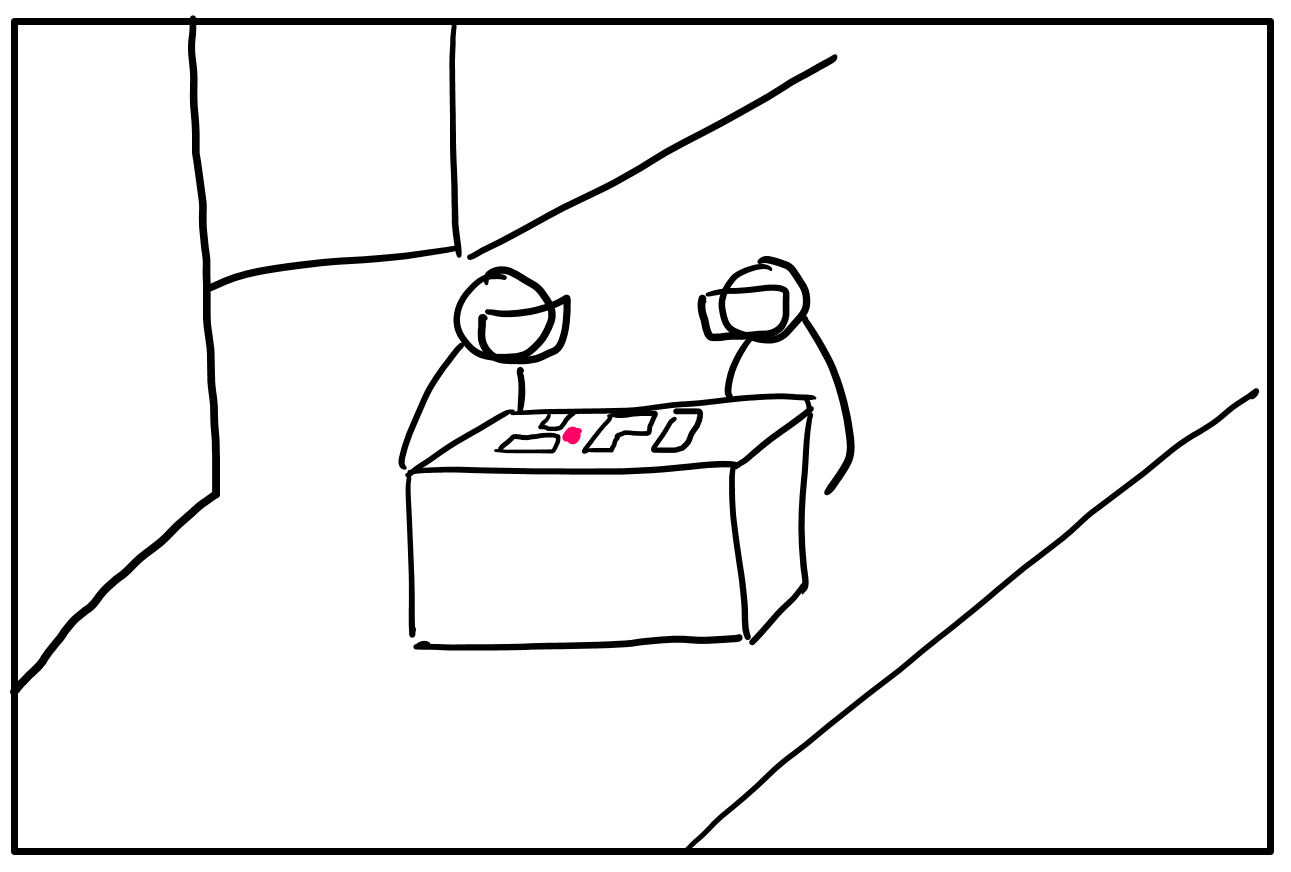
\includegraphics[scale=.2]{figures/comics/uncomfortable_collaboration.png}}
	\end{minipage}%
	\begin{minipage}{.25\linewidth}
		\centering
		\subfloat{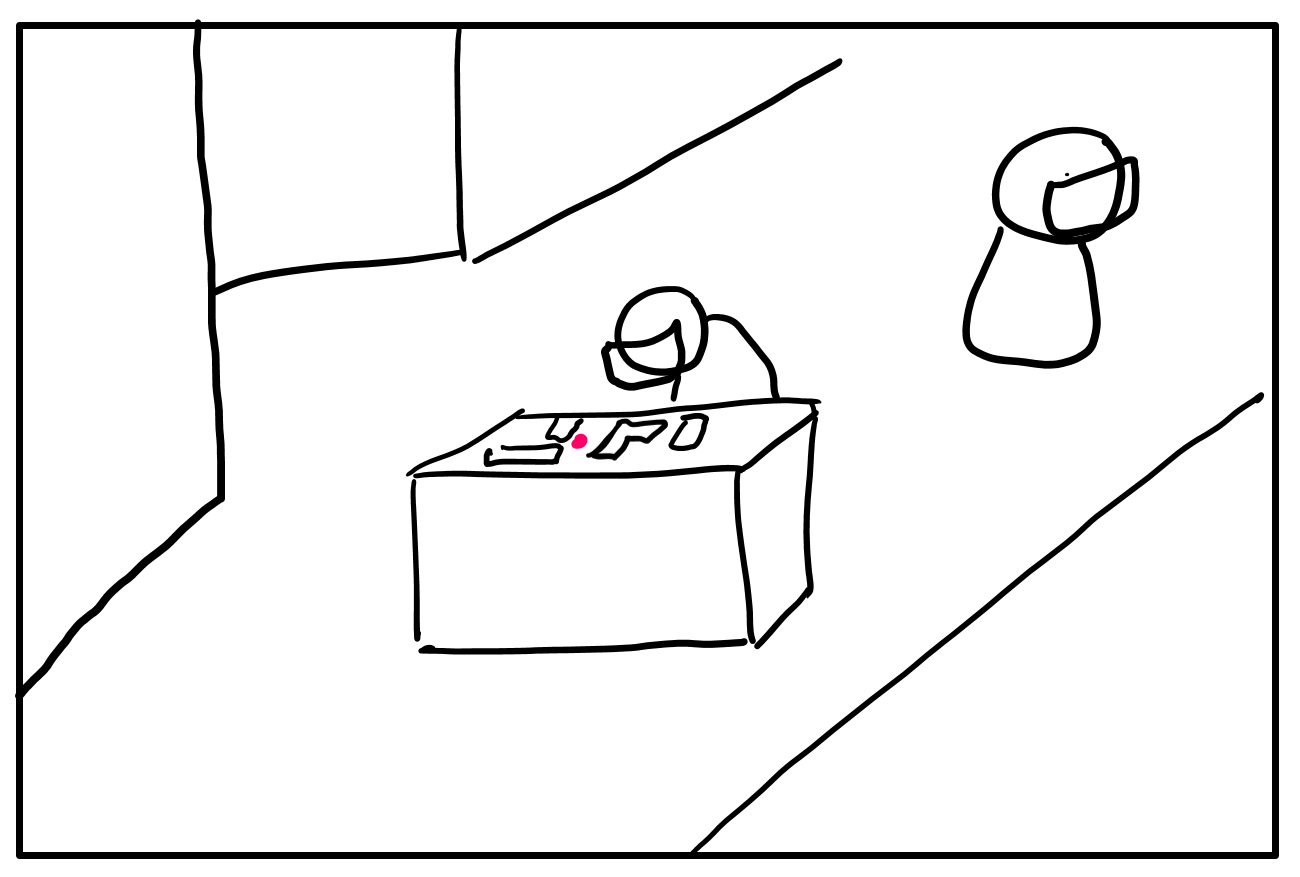
\includegraphics[scale=.2]{figures/comics/uncomfortable_collaboration2.png}}
	\end{minipage}%
	\begin{minipage}{.25\linewidth}
	\centering
	\subfloat{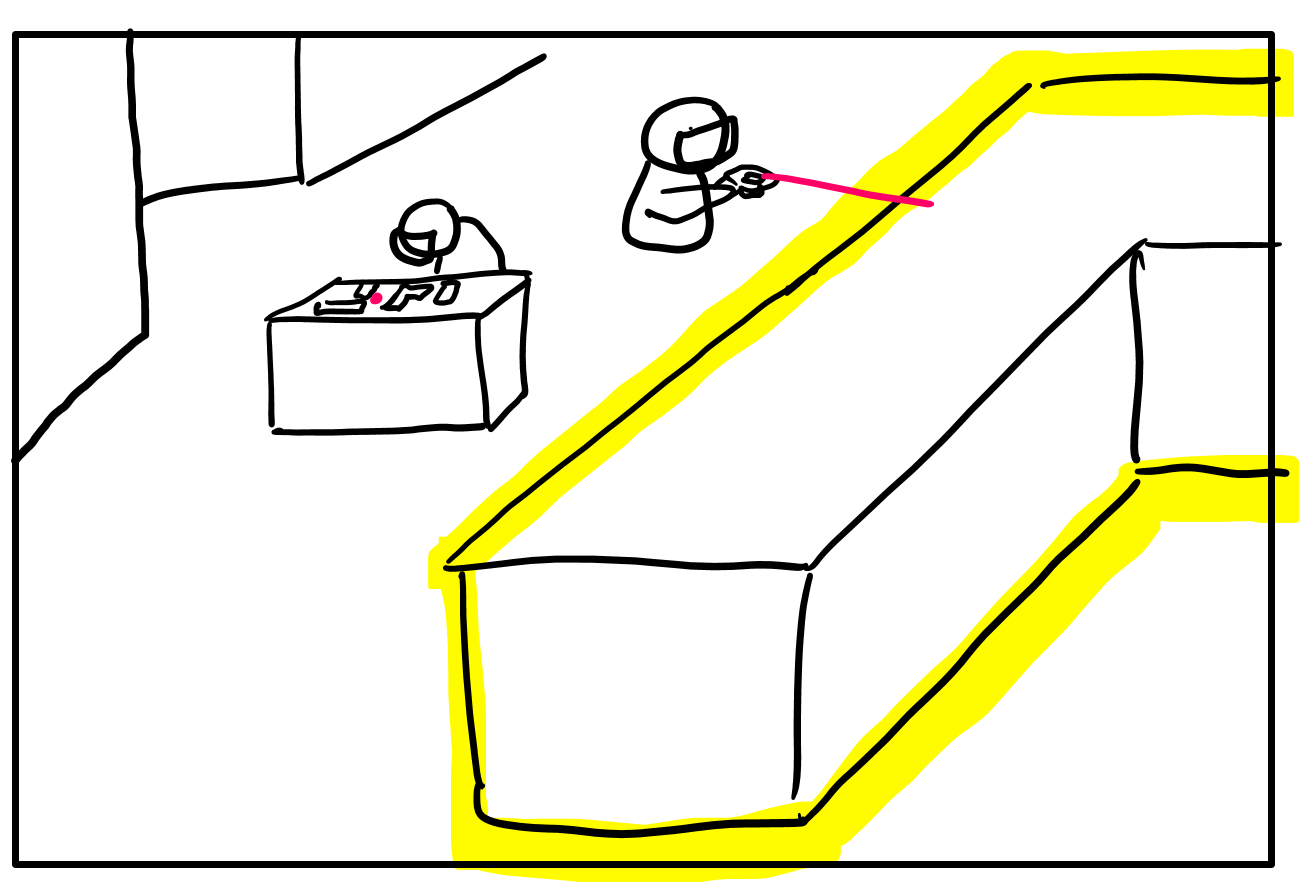
\includegraphics[scale=.2]{figures/comics/uncomfortable_collaboration3.png}}
	\end{minipage}
	
	\par\medskip
	\begin{minipage}{.25\linewidth}
		\centering
		\subfloat{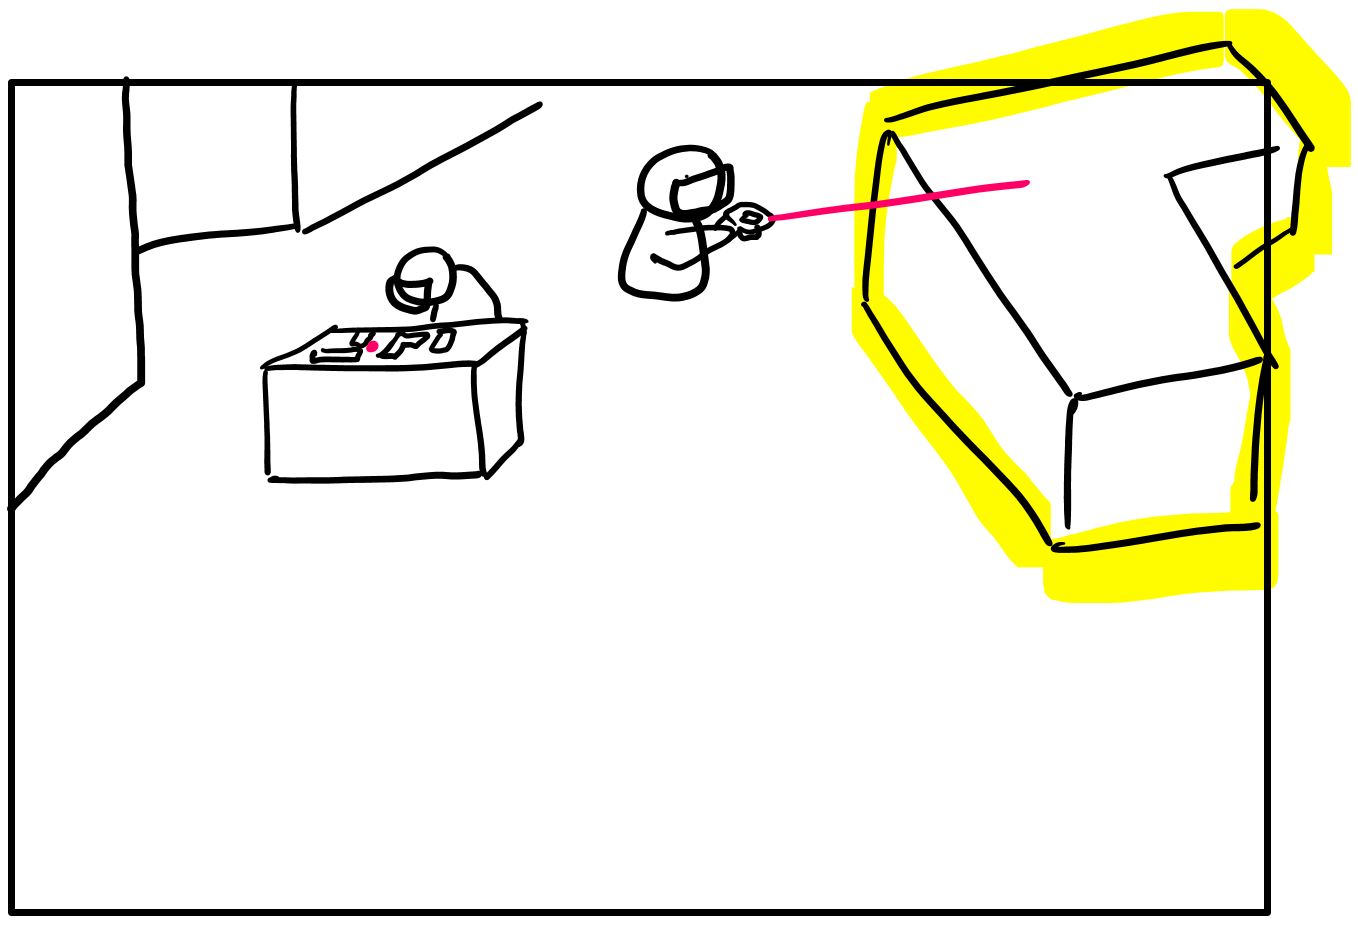
\includegraphics[scale=.2]{figures/comics/uncomfortable_collaboration4.png}}
	\end{minipage}%
	\begin{minipage}{.25\linewidth}
		\centering
		\subfloat{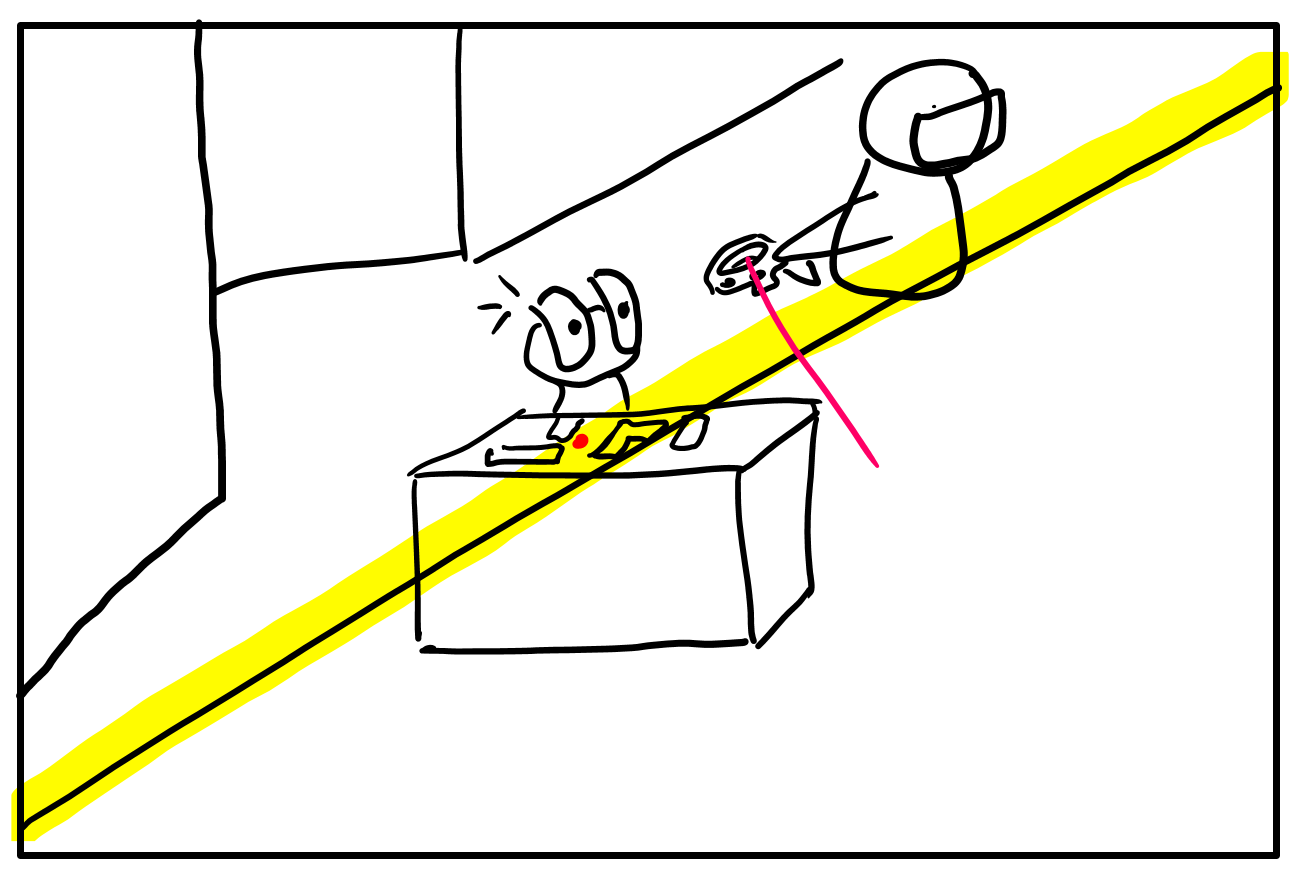
\includegraphics[scale=.2]{figures/comics/uncomfortable_collaboration5.png}}
	\end{minipage}%
	\begin{minipage}{.25\linewidth}
		\centering
		\subfloat{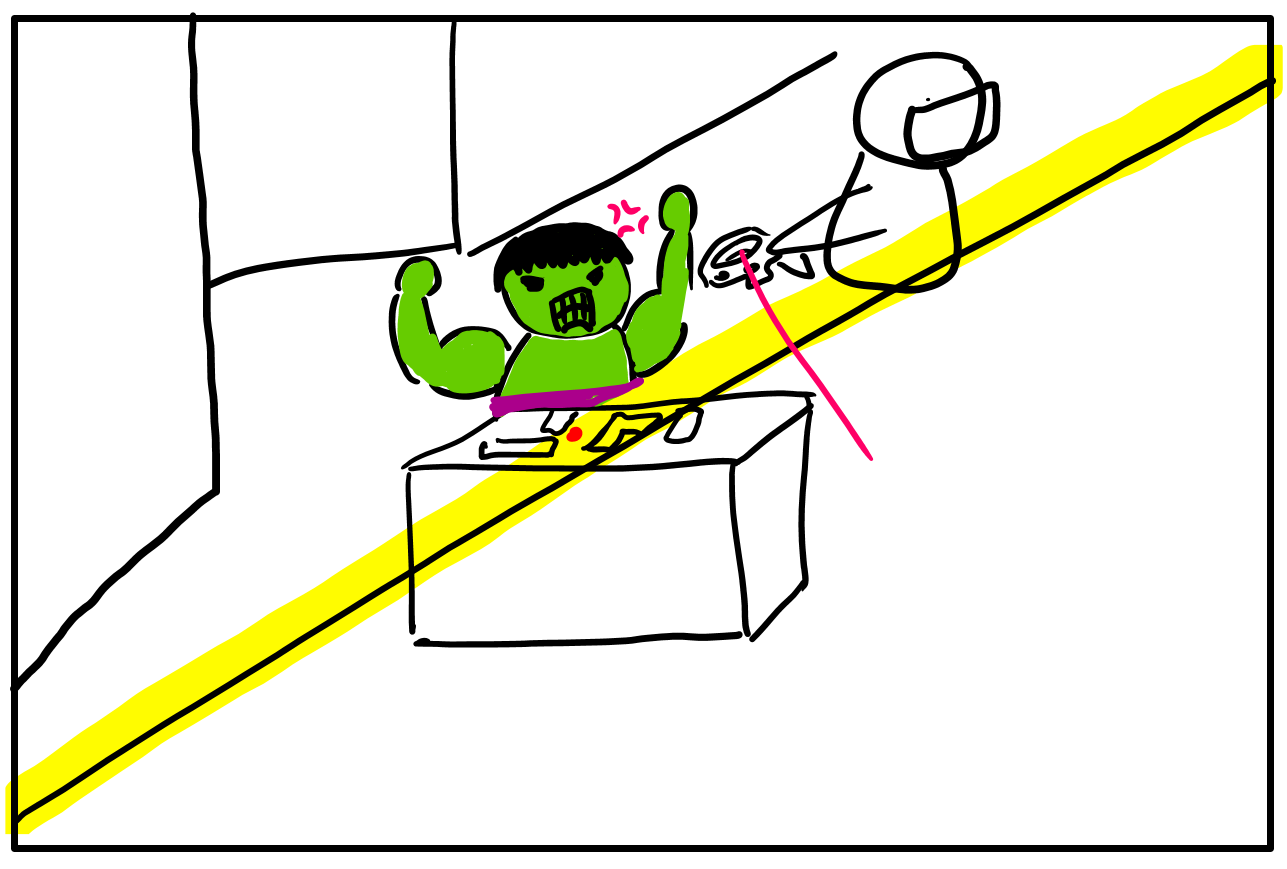
\includegraphics[scale=.2]{figures/comics/uncomfortable_collaboration6.png}}
	\end{minipage}
	
	\caption{Collaborators unaware of each other's actions}
	\label{fig:a1unawareofa2actions}
\end{figure}


%---------------Reference commands and structires

% \chapter{Introduction}\label{chapter:introduction}
% \section{Motivation: Teamwork is important. Creative thinking implies generation of ideas, collaboration, and communication. Virtual Reality (VR) is a great enhancement for creative thinking tool-set in architecture.}
%\subsection{Solution validation/evaluation in HCI: methods, and principles.}
\begin{comment}
Methodology: approach to solving the problem; chosen HCI methodology for the final evaluation - no idea
a. Chosen HCI evaluation methodology
\end{comment}


\begin{comment}
See~\autoref{tab:sample}, \autoref{fig:sample-drawing}, \autoref{fig:sample-plot}, \autoref{fig:sample-listing}.
\begin{table}[htpb]
  \caption[Example table]{An example for a simple table.}\label{tab:sample}
  \centering
  \begin{tabular}{l l l l}
    \toprule
      A & B & C & D \\
    \midrule
      1 & 2 & 1 & 2 \\
      2 & 3 & 2 & 3 \\
    \bottomrule
  \end{tabular}
\end{table}

\begin{figure}[htpb]
  \centering
  % This should probably go into a file in figures/
  \begin{tikzpicture}[node distance=3cm]
    \node (R0) {$R_1$};
    \node (R1) [right of=R0] {$R_2$};
    \node (R2) [below of=R1] {$R_4$};
    \node (R3) [below of=R0] {$R_3$};
    \node (R4) [right of=R1] {$R_5$};

    \path[every node]
      (R0) edge (R1)
      (R0) edge (R3)
      (R3) edge (R2)
      (R2) edge (R1)
      (R1) edge (R4);
  \end{tikzpicture}
  \caption[Example drawing]{An example for a simple drawing.}\label{fig:sample-drawing}
\end{figure}

\begin{figure}[htpb]
  \centering

  \pgfplotstableset{col sep=&, row sep=\\}
  % This should probably go into a file in data/
  \pgfplotstableread{
    a & b    \\
    1 & 1000 \\
    2 & 1500 \\
    3 & 1600 \\
  }\exampleA
  \pgfplotstableread{
    a & b    \\
    1 & 1200 \\
    2 & 800 \\
    3 & 1400 \\
  }\exampleB
  % This should probably go into a file in figures/
  \begin{tikzpicture}
    \begin{axis}[
        ymin=0,
        legend style={legend pos=south east},
        grid,
        thick,
        ylabel=Y,
        xlabel=X
      ]
      \addplot table[x=a, y=b]{\exampleA};
      \addlegendentry{Example A};
      \addplot table[x=a, y=b]{\exampleB};
      \addlegendentry{Example B};
    \end{axis}
  \end{tikzpicture}
  \caption[Example plot]{An example for a simple plot.}\label{fig:sample-plot}
\end{figure}

\begin{figure}[htpb]
  \centering
  \begin{tabular}{c}
  \begin{lstlisting}[language=SQL]
    SELECT * FROM tbl WHERE tbl.str = "str"
  \end{lstlisting}
  \end{tabular}
  \caption[Example listing]{An example for a source code listing.}\label{fig:sample-listing}
\end{figure}
\end{comment}
\glsresetall
% !TeX root = ../main.tex
% Add the above to each chapter to make compiling the PDF easier in some editors.

\chapter{Related Work}
This master thesis focuses on two broad topics, audio feedback and collaboration, which puts it at the intersection of the fields of \gls{hci} and \gls{cscw}, \gls{vr}, and \gls{cve}. I will start by introducing the field of \gls{hci}, and an important issue of human factors.

\section{HCI}
\parencite[Chapter~4.1.1]{jr_3d_2017} define \gls{hci} as "a field that seeks to understand the relationship between human users and digital technological artifacts and to design new, effective ways for humans to use computer technologies for all sorts of purposes". The word "computer", in this context, can mean anything from a smartphone to a desktop computer to a \gls{vr} setup, which in turn implies different interfaces: touch-based, 2D, immersive 3D, etc. Modern \gls{hci} deals not only with the human-computer interactions, but also pays emphasis on the computer as a medium for collaborative work, and hence "human-human interaction". The goals pursued in \gls{hci} are not to simply understand the interactions we already use today, but to design the new interactions, be it through novel hardware and software solutions or innovative application of the existing ones. 
%Lately,\gls{hci} experienced a shift from focusing on the \gls{ui} to the \gls{ux}, which encompasses \gls{ui} and deals with the ecology that the system exists in (social context, cultural differences, skills and emotional state of the users, and so on).

\subparagraph{Human Factors}
One of the principal reference points in \gls{hci} is the notion of human factors, or as it is also called, ergonomics. Two of the three main factors are perception and cognition \parencite{jr_3d_2017}. A a significant part of this thesis resides with these two factors. The third factor is Physical Ergonomics, which is used to design comfortable and effective interfaces with regard to the human physiology. It is not highly relevant for this work, and thus will be addressed only scarcely. A review of physical ergonomics factor can be found in \parencite[Chapter~3.5]{jr_3d_2017}.

% 3.1 Intro: definition and examples

% 3.2 Information processing: how human IP is tied with the main human factors, the graph; short, one-paragraph, explanation of everything in the graph
If we consider the interactions with the outside world, everything we do happens based on the information we get from our environment and body. \parencite{jr_3d_2017} argue that processing of this information can be mapped to the aforementioned human factors (see Fig. \ref{fig:informationprocessingloop}).
At the perception stage, the outside events or stimuli are first received through the sensory system, and then interpreted and matched with experience from the past. Based on the interpreted information, an action can be taken, or this information can be saved in the working (short-term) memory. 
%Short-term memory has limited capacity, and is directly affected by the attention. Contrary, long-term memory is vast, is not directly affected by the attention, and used to store information about the world. 
Based on the actions taken, the responses can be fed back into the information processing loop.

\begin{figure}
	\centering
	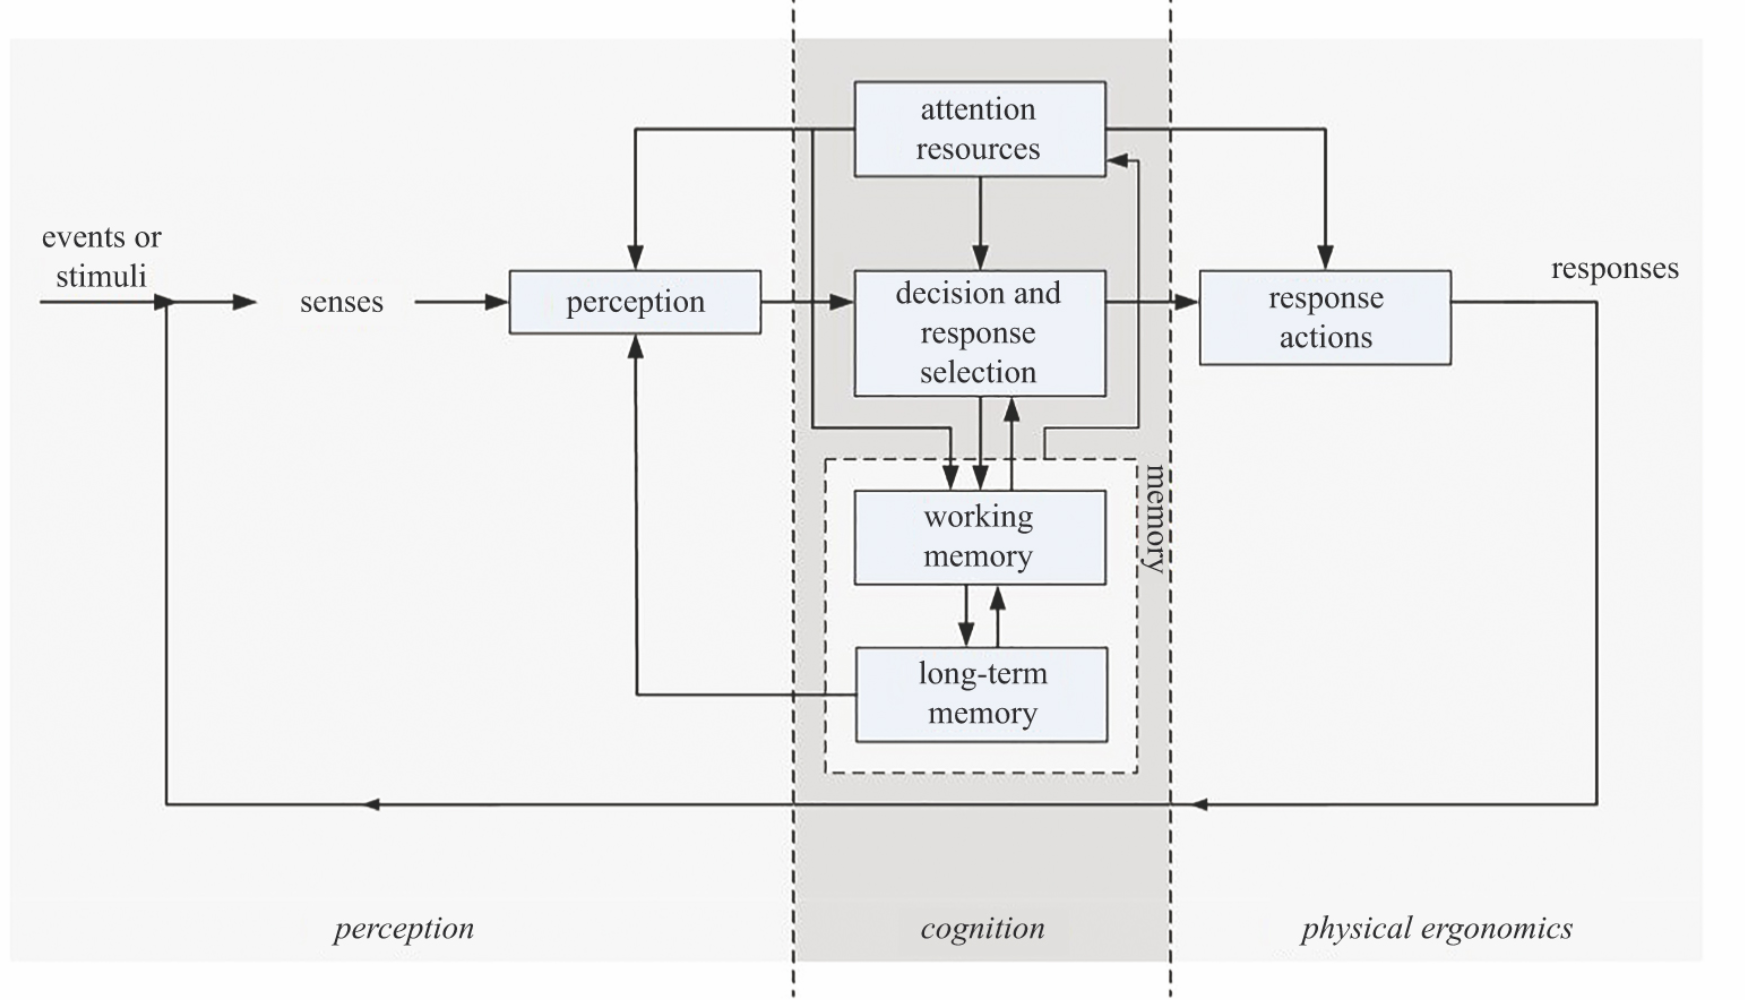
\includegraphics[width=0.7\linewidth]{figures/placeholders/information_processing_loop}
	\caption{Information processing loop. Source: \parencite{jr_3d_2017}} % TODO: redraw
	\label{fig:informationprocessingloop}
\end{figure}

% 3.3 Perception: responsible for auditory perseption and comprises one part of this work (perceptual mechanisms; types of perceptual cues; sensory substitution and multisensory processing)
Perception factor deals with all information, available to us through our senses: visual, auditory, somatosensory (haptic) and chemical sensing systems. It is responsible for receiving and interpreting this information.
One of the useful features of our sensory system is that different senses can substitute each other, for example, somatosensory information can be substituted with sound in systems, where haptic feedback is not available. Multisensory processing is another useful feature describes situations, where perception in one sensory channel improve the perception in the other (for example, when you notice someone waving at you and suddenly start to hear what they are saying).
Previously, I hypothesized that additional audio feedback may lead to an overall improvement of the satisfaction with the collaboration experience. This is a topic that lies partially in the realm of perception: sounds have to be first heard and matched to the previous experience and memory.

% TODO: re-read this
% 3.4 Cognition governs awareness, a state of noticing certain details about the environment, people, or tasks.
Moving on to cognition, it is defined as "the driving force behind the generation and usage of knowledge" in \parencite{jr_3d_2017}. This factor is responsible for our thought process and is directly linked to the perception and attention. The study of cognition is a study of how these thought processes function and how cognition effects our interactions with the environment.
For a user to be able to comprehend what is happening in the environment, they have to be aware of it, first. Cognition governs the concept of awareness. There are different types of awareness, but all of them concern the analysis and design of systems in such a way that they help users stay informed about the environment (for example, things like other people, tasks, or the workspace).
%The main cognition problems that occur in the designed interface are mental (cognition) load and human error. The former can occur due to the properties of the task (difficulty, priority, etc.), or exceeding the attention and processing resources of an individual. The latter can be generally described as a lack of success in performing the task, and can be also caused by the perception and physical ergonomics issues.

% 3.5 Physical ergonomics: "enables us to design systems that can be used comfortably and effectively". Not strictly relevent to this work.. Except maybe for the controlls (participants complained about the mapping), but this should go into summary. Explores 
\begin{comment}
The last factor, physical ergonomics, puts emphasis on the affordances of the human body in designing different \gls{hci}s: its components and their function, different motion types, sensory-motor distribution, and posture. The typical issues addressed for this factor are fatigue and user comfort.
\end{comment}

% Example: 1.1 sound waves -> 1.2 sound -> 1.3 car signaling -> 2.1 I'm on the road -> 2.2 it can hit me -> 2.3 I should get away! -> 3. action
To see how the information processing loop maps to the real situations, let me go back to the original use case of two users interacting in the same immersive \gls{vr} environment: User 1 is concerned with his own task and does not notice the other user, User 2. The latter starts translating buildings in the environment. This time, the movement of buildings is followed by an audio feedback.
Considering User 1 is familiar with what different sounds in the environment correspond to, the stages of the information processing loop for them will look as follows:
\begin{description}
	\item[Perception:] \hfill
		\begin{enumerate}
			\item Waves of frequency 20 Hz - 20 kHz are received at the outer ear;
			\item The waves are interpreted as sound;
			\item The sound is classified as that of a moving building.
		\end{enumerate}
	\item[Congition:] \hfill
		
		\begin{enumerate}
			\item User 1 realizes that someone is translating a building;
			\item User 1 decides to get away from the building's moving trajectory, or saves the information that there is a building moving in the environment and is less stuttered if it happens to move through them or close to them.
		\end{enumerate}
	\item[Physical Ergonomics:] \hfill
			
			The person gets off the building's moving trajectory or continues working on the task with newly acquired knowledge.
		
\end{description}

\section{Collaboration in VR}

\paragraph{VR}
% May also be addressed in Chapter 2. 3D User Interfaces: History and Roadmap and in the part about the HMDs
% Next we will take a look at the history of \gls{vr}, which is relevant for the both, \gls{hci} and \gls{cve} research
The recent surge of the \gls{vr} technology made it associate almost exclusively in consumer eyes with Oculus Rift- or HTC Vive-type of devices that use precise sub-millimeter tracking for the \gls{hmd} and controllers, stereo rendering, high fidelity displays, and wide-angle field of vision. And while this is exactly the kind of \gls{vr} medium we are concerned with for this project, it is useful to shortly consider the scope and terminology of the field.

% \gls{vr} aims
\parencite{jr_3d_2017} define \gls{vr} as an "approach that uses displays, tracking, and other technologies to immerse the user into the \gls{ve}". A \gls{ve} is an artificial (usually 3D) environment that allows navigation, and where the view is controlled by the user in real-time. The authors note that the terms \gls{vr} and \gls{ve} are often used interchangeably in practice. 
In actuality, the recent advances in the \gls{vr} technology were not as drastic as they might seem at the first glance. \parencite{slater_immersion_2018} points out that the field had already experienced a similar level of development with head- and hand-tracking, and immersive displays in late 1980s-early 1990s. The difference with the current situation is the price (the old devices might have cost thousands or tens of thousands of dollars, as opposed to hundreds of dollars for today's setups) and the advances in computer graphics.
Dependence on advanced computer graphics has always been a distinct feature of the \gls{vr} field. However, a large number of fairly different systems were also classified as \gls{vr}, among them: desktop VR applications (see \parencite{churchill_collaborative_1998}, Example Projects section), non-visual \parencite{ammi_intermodal_2015}, and highly immersive (\parencite{davidson_greenspace_1996}, \parencite{greenwald_cocoverse_nodate}, \parencite{lena_real-time_nodate}, \parencite{kulik_virtual_2018}). The binding factor being the aim to immerse one of the senses. \parencite{slater_immersion_2018} defines the "immersion" property in \gls{vr}. Through it he shows how different systems can be combined under the same term - immersion is defined "as an objective property of a system, and higher or lower immersion as the extent to which a VR system can support natural sensorimotor contingencies for perception". He gives an example of a desktop \gls{vr} application, where immersion disappears as soon, as the user turns his gaze away from the screen, and an application using a tracked \gls{hmd}, which has higher immersion, because the illusion is not broken when you look away.

%The most popular are still.. The combining factor is the attempt to trick our senses into believing we are ..
% Immersiveness: desktop VR (see Churchill, example systems), non-visual (Ammi&Katz), surround-screens (Kulik, Lena), and HMDs (GreenSpaceII, Greenwald_CocoVerse).

% vr in the field of collaboration rarely means immersive \gls{vr}  
%Generally, and in collaborative research specifically, the terms \gls{ve} and \gls{vr} are used interchangeably. In this work I will denote

% VR sickness

% Terminology: further "immersive vr environment" would be addressed as "immersive vr", or "immersive ve" based on whether the Oculus Rift- and HTC Vive-like devices are used as the medium, or not.


\paragraph[]{CSCWs and CVEs}
Digital collaboration has been addressed in multiple research areas and has a tangled history. Traditionally, it is considered a problem of the \gls{cscw} field, but there was time when it was debated whether it can be considered a distinct research area. 
\gls{hci} did not always address the use of a computer as a medium for human-to-human collaboration, and \parencite{bannon_perspectives_nodate} writes that the inability of \gls{hci} to address the use of a computer as a medium for human-to-human communication, and in doing so to satisfy the requirements of a group in software design, had sparked the first shift towards the research on human-computer-human interaction (HCHI). 
%The main focus of the \gls{hci} is on providing the proper interface for the interaction between an individual and a computer. 
This shift was originally supported by the \gls{cmc} movement. However, it was mostly a reactive measure, aimed at analyzing how the existing solutions integrate in the actual workspaces, instead of gathering material to help future design and re-design of collaborative systems. The proactive measure came through the establishment of the \gls{cscw} field. The special term "groupware" was coined, which indicated the emphasis on software to support the work of users in groups and their established workflows.

%[CVE - churchil,greenwald]
The next paradigm shift started to happen in the late 1990s, where the already established field of \gls{cscw} started facing the problems of its own, specifically when trying to apply the approach to more open-ended and creative tasks. \parencite{churchill_collaborative_1998} argue that the \gls{cscw} approach at the time was better at addressing the routine tasks, such as those with clear requirements for the form of the input and output data: video conferencing, email, co-authoring applications, shared drawing applications, etc. In contrast, the tasks, like design, where users spend significant amount of time discussing and negotiating suffered from imposing a rigid structure early on. In answer to this problem, an approach emerged that has its origins in the domain of \gls{vr} - the \gls{cve}. Churchill and Snowdon describe \gls{cve}s as "distributed, virtual reality that is designed to support collaborative activities". The main difference from the \gls{cscw} was in the freedom of self-expression, interaction with common objects (artifacts) in the scene, and communication. The comparison of appearance of these types of systems can be observed in Fig. \ref{fig:approaches_to_collaboration}, and the differences are instantly noticeable: while \gls{cscw} looks like a traditional desktop application, the \gls{cve} reminds more of a computer game, than a tool to promote collaboration during remote collaboration. 

\begin{figure}
	\centering
	\hfill
	\subfloat[CSCW]{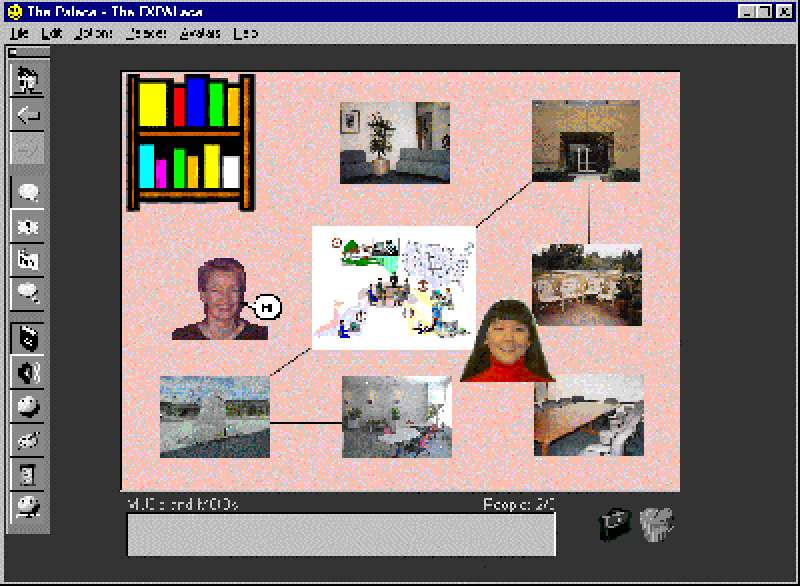
\includegraphics[width=0.4\linewidth]{figures/churchill_snowdon_cscw_vs_cve/A-room-created-using-The-Palace-with-two-avatar-embodiments}}
	\hfill
	\subfloat[CVE]{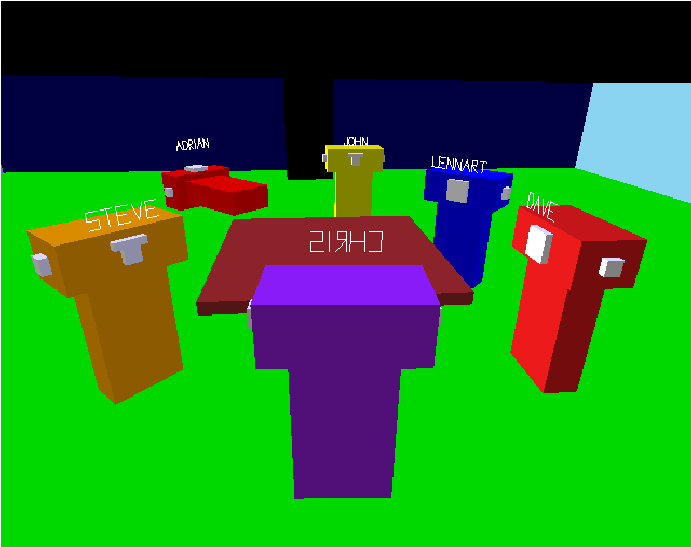
\includegraphics[width=0.4\linewidth]{figures/churchill_snowdon_cscw_vs_cve/Embodiments-in-MASSIVE-1}}
	\hfill
	\caption{Approaches to collaboration. Source: \parencite{churchill_collaborative_1998}}
	\label{fig:approaches_to_collaboration}
\end{figure}

%[immersive CVE - greenwald cocoverse]
The latest leap in digital collaboration was initiated with the introduction of the aforementioned immersive \gls{vr} systems, like Oculus Rift and HTC Vive. The new hardware interfaces proved to be less foreign, and not impose high attention load for operation (the initial reason why \gls{cve}s found much broader application in gaming, than in distributed workspaces), which reignited the interest for the application of the medium in various, like collaborative learning \parencite{greenwald_cocoverse_nodate}. 
%More detail on the history of the \gls{cve}s from the introduction to the topic by Churchill and Snowdon to the current day \gls{hmd}s for immersive \gls{vr} can be found in \parencite{greenwald_technology_2017}.

\begin{comment}
\paragraph{Terminology}
To disambiguate the further discussion in this thesis, I will use the following terminology:  
\begin{description}
	\item[immersive \gls{vr}] refers to the experiences through Oculus Rift-like mediums;
	\item[surround-screen \gls{vr}] refers to the use of surround-screen displays instead of tracked \gls{hmd}s to deliver the \gls{vr} experience;
	\item[\gls{ve} application] refers to the less immersive, desktop \gls{vr} setups;
	\item[shared (or collaborative) \gls{vr} environment] refers to collaborative counter part to the "immersive \gls{vr}";
	\item[digital collaboration] refers to all and any of the different types of collaboration through a digital medium: \gls{cscw}, gls{cve}, collaborative \gls{vr}, etc.
\end{description}
\end{comment}

\paragraph[Bridge]{}
In this chapter I gave an overview of the relevant topics from the fields of \gls{hci} and collaboration. The following two chapters will build upon this, and explore the properties and applications of audio and the role of \gls{wa} in presenting the user with this information.

\begin{comment}

\begin{figure}
	\centering
	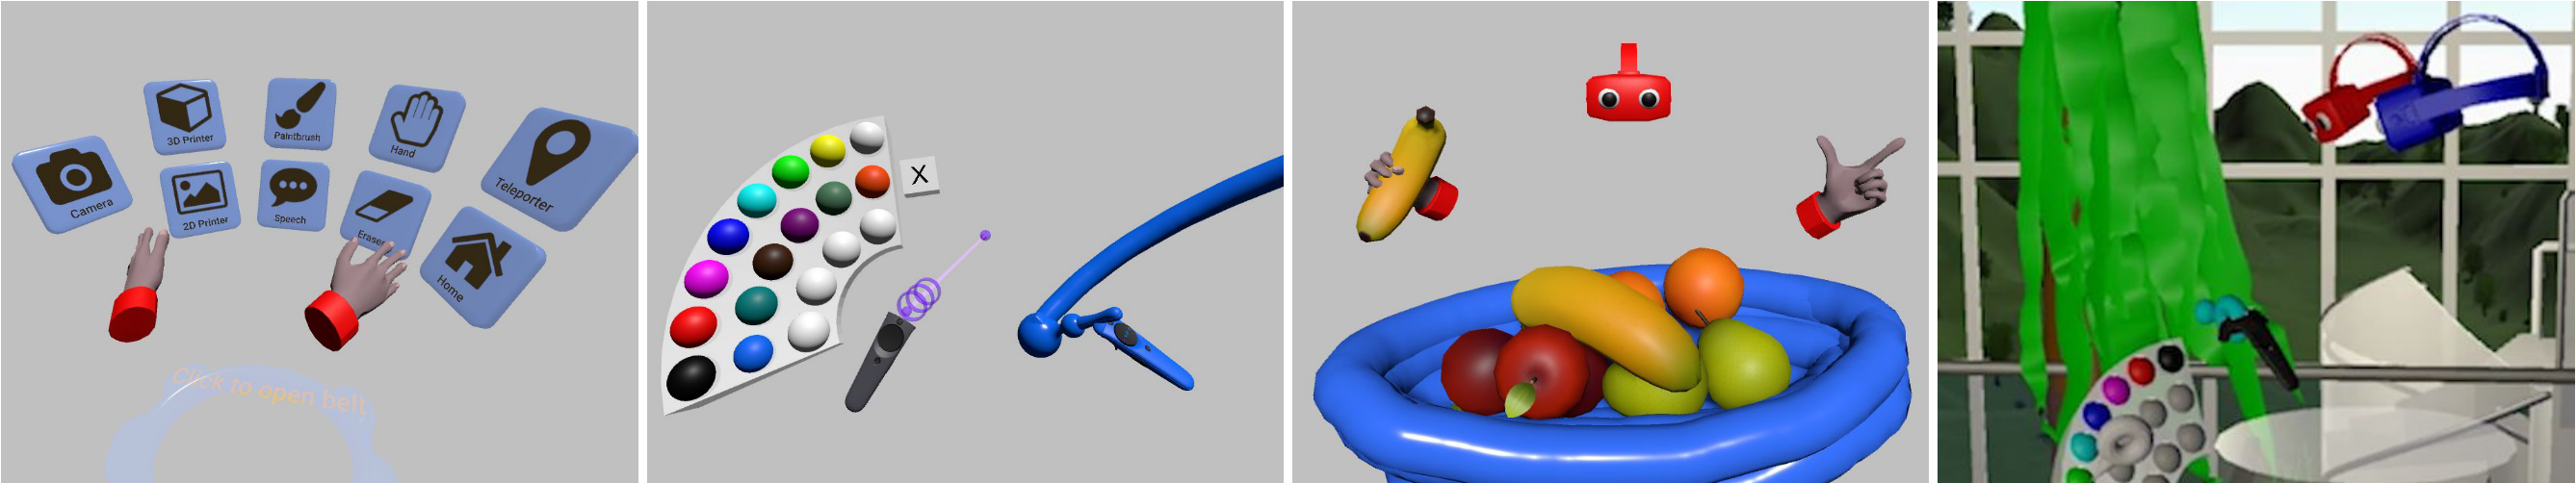
\includegraphics[width=0.7\linewidth]{figures/Cocoverse}
	\caption{CocoVerse, environment affordances and avatars (Source: \parencite{greenwald_cocoverse_nodate})}
	\label{fig:cocoverse}
\end{figure}

\paragraph[Related Work]{}
We will now take a look at the some of the problems that were appraoched in the domain of digital collaboration.

% Interactions and navigation // THis is more a single-player problem
% Greenspace II
Some collaborative projects address the question of interactions with shared artifacts. From the earlier studies, \parencite{davidson_greenspace_1996} present an immersive \gls{vr} system with 6 \gls{dof} tracked head and hand movements that facilitates design review and discussion of the architectural design decisions. This was much an exploratory study, where participants got to explore the design of a 3D environment in an interactive fashion. The authors report their findings on the navigation, communication, manipulation and some social affordances of the resulting application.
% Lena
\parencite{lena_real-time_nodate} presents a research into what constitutes an interactions in \gls{vr} and utilizes the findings in the \gls{cdp} project to connect two "different realities": an interactive table computer and a CAVE-environment. Intentional non-verbal communication and embodiment are also explored.

% Presence
% CocoVerse
Next popular topic of research is the different types of presence, also described as a feeling of "being there".
Greenwald et al. (\parencite{greenwald_cocoverse_nodate}, \parencite{greenwald_investigating_2017}, \parencite{greenwald_technology_2017}) are exploring the utility of shared immersive \gls{vr} for collaborative learning and co-operation. Authors present a system that is the first of its kind in the research community multi-user framework for collaboration and co-creation, CocoVerse (Fig. \ref{fig:cocoverse}). The topics addressed are: social presence (the quality of the medium in convincing users in the salience of the others, present in the same \gls{ve}), co-presence (psychological and emotional interactions between the users), embodiment (how users are represented), as well as non-verbal communication (i.e. through gestures).
Even though, it is already closer to our initial problem formulation, this stream of research focuses mostly on the phase where users' attention is equally engaged on the same subject.

% Awareness
\parencite{gutwin_descriptive_2002} split a collaborative situation into two parts: the domain task and the collaborative part. Ammi and Katz, in their study on communication via audio and haptic feedback in abstract and non-visual environments, prior to implementation, derive requirements to the individual (domain) and collaborative parts of the application \parencite{ammi_intermodal_2015}. The former include the concept of \gls{sa}, and the later consists of process and \gls{wa}.
% Situation & Workspace awareness differences
\gls{sa} is defined by Endsley as: "the perception of the elements in the environment within a volume of time and space, the comprehension of their meaning, and the projection of their status in the near future" \parencite{endsley_situation_1988}. In-fact, \gls{wa} is a special type of \gls{sa} in shared workspaces. The first difference is that the focus of the \gls{sa} on the domain task only is extended with the focus on collaborative task. Secondly, the extreme flow of information that is typical for \gls{sa} due to its roots in the jet fighter simulations, is reduced in volume to match the use case of shared collaboration between colleagues. Main reason for this is, as authors put it: "sorting slides on a table does not seem very similar to air combat in a jet fighter" \parencite{gutwin_descriptive_2002}.

% Similaritites
The part that is similar about the two types of awareness, and that makes this topic interesting in the context of current thesis, is that in both cases users are unable to gather the information they need. If, in case of a jet fighter simulation, the pilot is simply overwhelmed by the sheer volume of the information presented, then in the sorting slides task the users is failing to gather information due to the fact that the system does not present them with adequate awareness information by default.

% Workspace awareness framework: types of communication
The authors go ahead and introduce a descriptive framework to help groupware
designers determine what types of awareness presentations to include in their systems, and allow the comparison of the systems based on the extent to which they promote \gls{wa}.
The framework consists of three parts:
\begin{description}
	\item[Part I] What information makes up \gls{wa}?
	\item[Part II] How is the \gls{wa} information gathered?
	\item[Part III] How is \gls{wa} used in collaboration?
\end{description}

The second part of the framework provides insights about the different sources of \gls{wa} information: 
\begin{enumerate}
	\item Bodies and consequential communication;
	\item Artifacts and feedthrough;
	\item Conversation, gesture, and intentional communication.
\end{enumerate}
While 1 and 3 can be summarized as non-intentional and intentional communication, feedthrough is a mechanism of interest for our purposes, as it implies that artifacts (objects in the \gls{ve}) give off information (audio, visual, etc.) when manipulated, which simultaneously serves as a feedback to the person performing the manipulation and as a notification to the others present in the workspace.
% Gutwin_chalk_2011
The authors utilize this mechanism in their study on the use of synthesized audio to promote to promote \gls{wa} in a shared chalkboard application \parencite{gutwin_chalk_2011}. In the systems, users are tasked with tracing a 2D shape (i.e. an outline of a ship), which is accompanied with an auditory feedback. There are two types of users in this environment - the real one (participant) and the simulated (user agent). The later is responsible for drawing shapes in the off-screen part of the workspace, while the former has two tasks - the primary and secondary. The primary task is to trace a given shape, and the secondary is to report that they noticed changes to the environment caused by the user agent. Among other topics, the authors explore the effect different awareness presentations and their combinations (type of auditory feedback, availability of the minimap of the environment, workspace clutter, and attention load) have on the \gls{wa}. They report a substantial increase in awareness due to the use of audio to convey information.
\begin{figure}
	\centering
	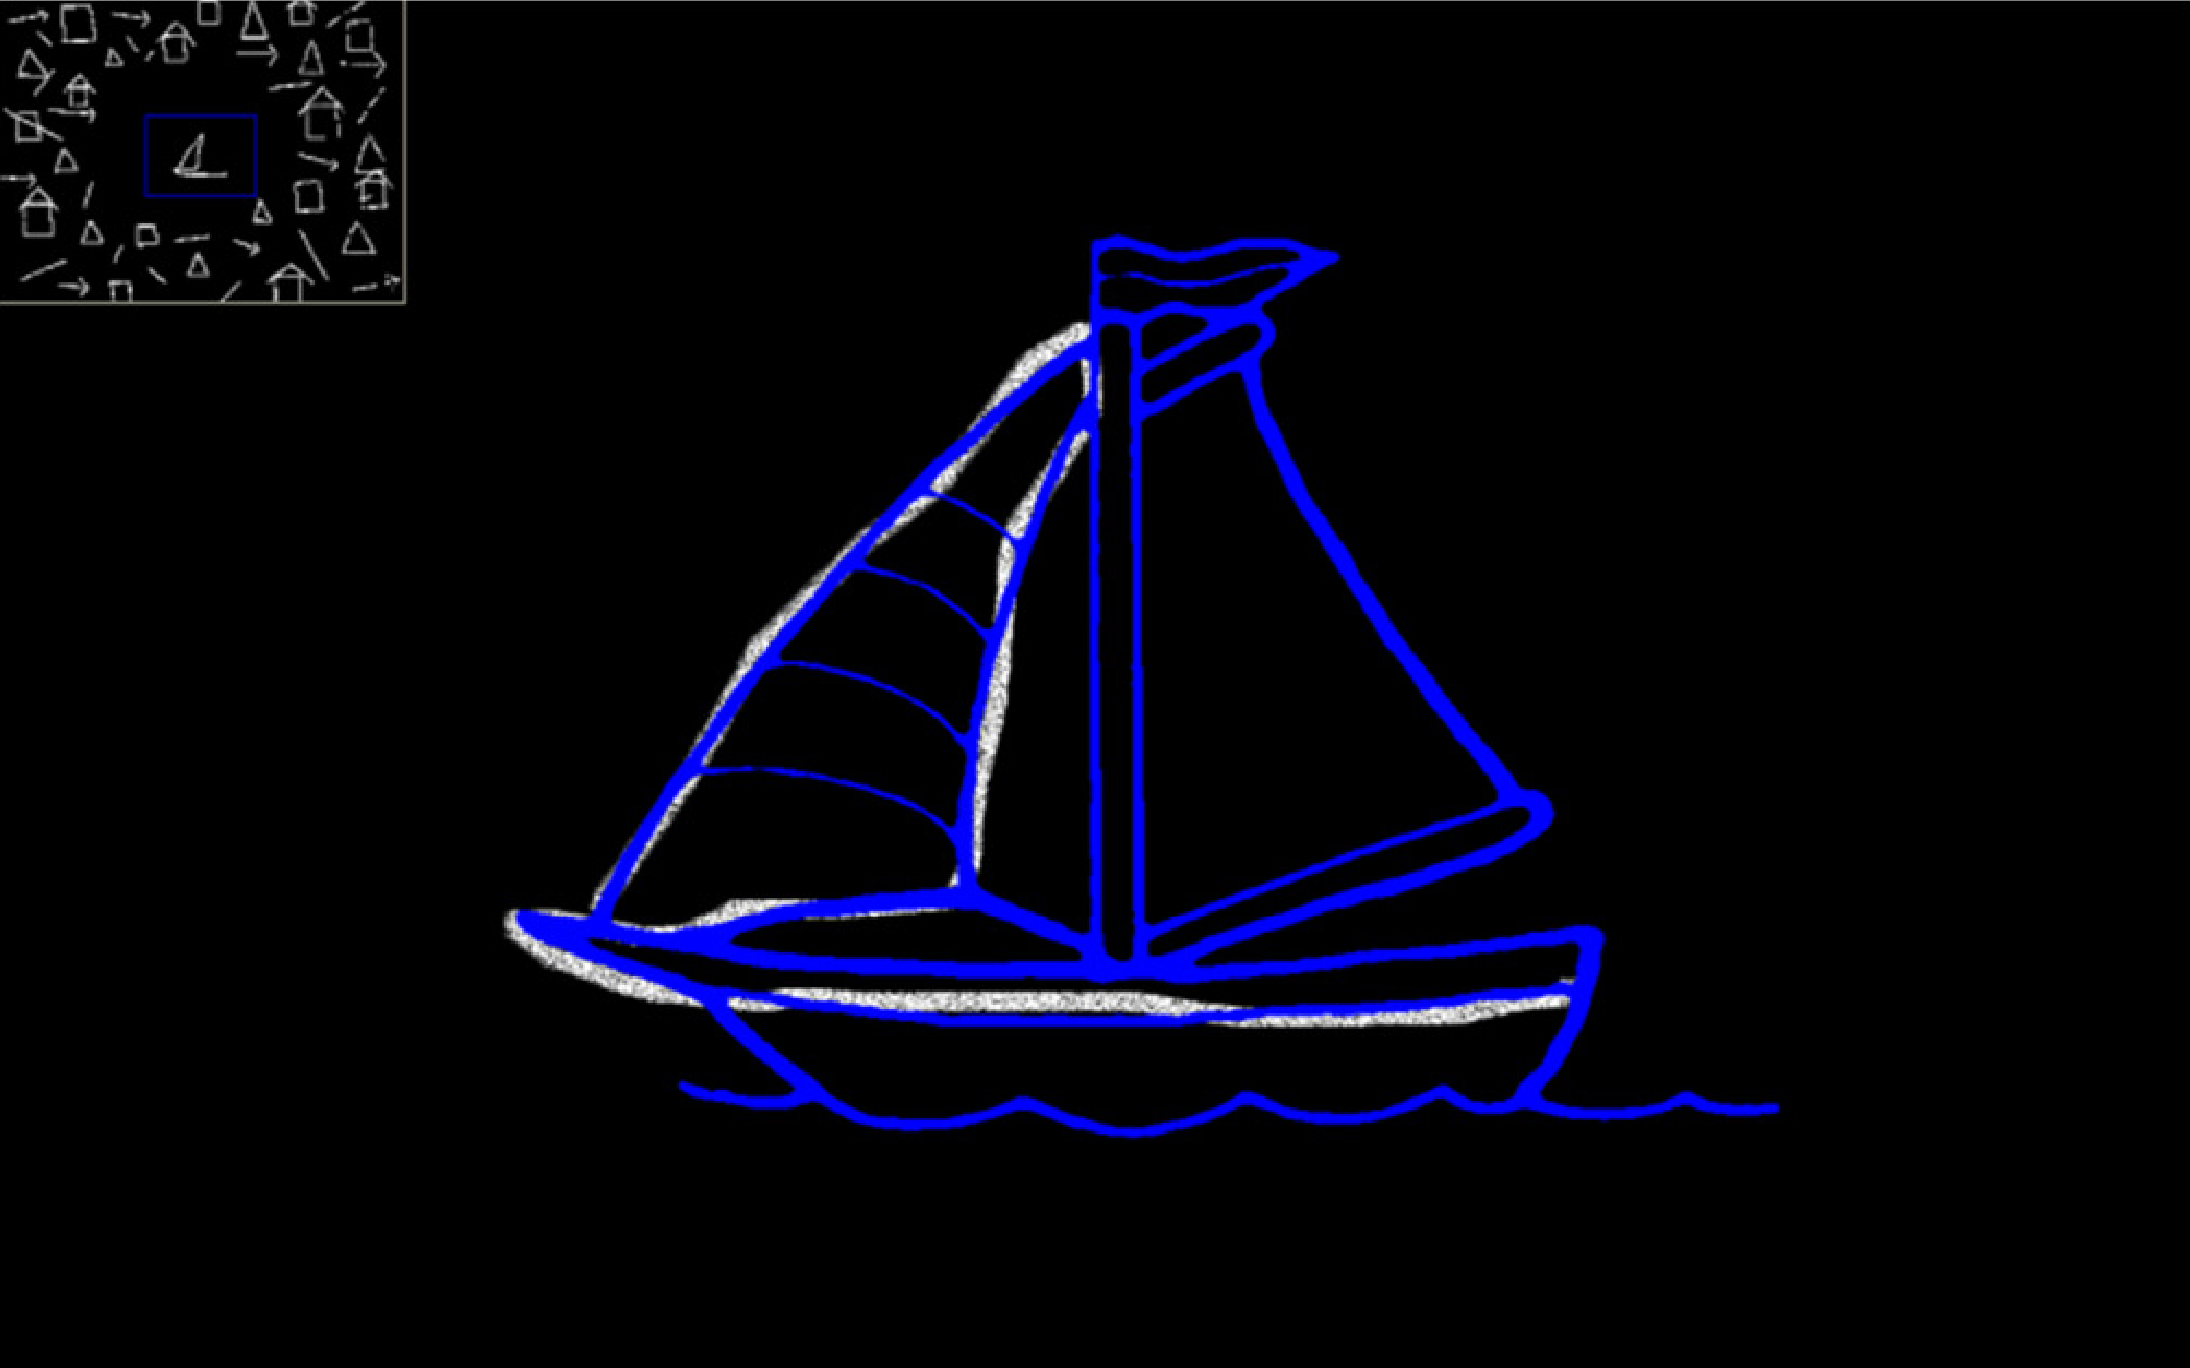
\includegraphics[width=0.7\linewidth]{figures/gutwin_chalk_2011}
	\caption{Shared chalkboard application, tracing shape and minimap (Source: \parencite{gutwin_chalk_2011})}
	\label{fig:gutwinchalk2011}
\end{figure}

In the next chapter we take a closer look at some of sound properties that can be utilized our application to counter the unexpected changes to the environment and enhance the \gls{wa}.

\end{comment}

\begin{comment}


% Gutwin
Gutwin and Greenberg explore the effects of synthesized sound in a shared chalkboard \gls{cscw} on the \gls{wa} ("the up-to-the-moment understanding of another person’s interaction with a shared workspace"). In this system two users are sharing a 2D workspace (a chalkboard). One user was real (participant) and another was simulated (agent). The agent would draw in an off-screen part of the workspace, this activity was accompanied by a synthesized sound. The real user had two tasks - primary and secondary. The former was to trace a given 2D shape (i.e. an outline of a ship) in their part of the shared workspace, and the later was to indicate whether they noticed the changes caused by the agent. % TODO: I don't look so deep into other studies
The authors study the extent of the ability of auditory cues to signal changes in the workspace, in comparison and in combination with a minimap.

% Ammi & Katz
\parencite{ammi_intermodal_2015} study the application of abstract and non-visual \gls{vr} environments in the context of improving communication. The system facilitates a collaborative search of targets with the help of audio and haptic feedback. The authors work out a specification for both the individual and the collaborative aspects of the task. The concept of \gls{sa} is used to address the former, and workspace and process awarenesses - the later.

As we have seen, even in the fields of \gls{cscw} and \gls{cve}, a broad range of topics can be addressed with respect to collaboration..
We have viewed non-visual, 2D, immersive \gls{vr} environments 
These are only some..
We will now take a closer look at the awareness approach, as it provides us with..
% Intentional and unintentional communication? Communication with aware person and unaware person - Nah, the difference is in the type of the task that is being conducted. In gutwin the domain task is being explored, while the others explore the collaborative part.

Collaboration can be approached in different ways, depending on the task at hand. More traditional approach is with \gls{cscw} systems, it works well when the task is routine and just requires either information exchange, or an execution of a pre-defined task \parencite{churchill_collaborative_1998}. For more creative and non-trivial tasks, which can be obscured by enforcing a certain workflow early-on, an approach using \gls{cve} is more appropriate.

\paragraph{}
% CVEs
One of the origins of \gls{cve}s is the field of \gls{vr}. This is mostly due to the aim  to allow users creative freedom, and reduce the learning curve by providing an intuitive interface. The task of a \gls{cve} is to facilitate communication and collaboration. They allow synchronous and asynchronous task execution, and provide the support for real-time sharing of visual artifacts \parencite{churchill_collaborative_1998}.

\subparagraph{}
% Cocoverse, Greenwald - first system of this kind in the research community
A good and concise review of the history of the \gls{cve}s can be found in \parencite{greenwald_technology_2017}. The state of art in the area of CVEs was reached by one of the authors, in \parencite{greenwald_cocoverse_nodate} and \parencite{greenwald_investigating_2017} he presents CocoVerse - a shared immersive \gls{vr} environment for local collaboration and co-creation (Fig. \ref{fig:cocoverse}).

\begin{figure}
	\centering
	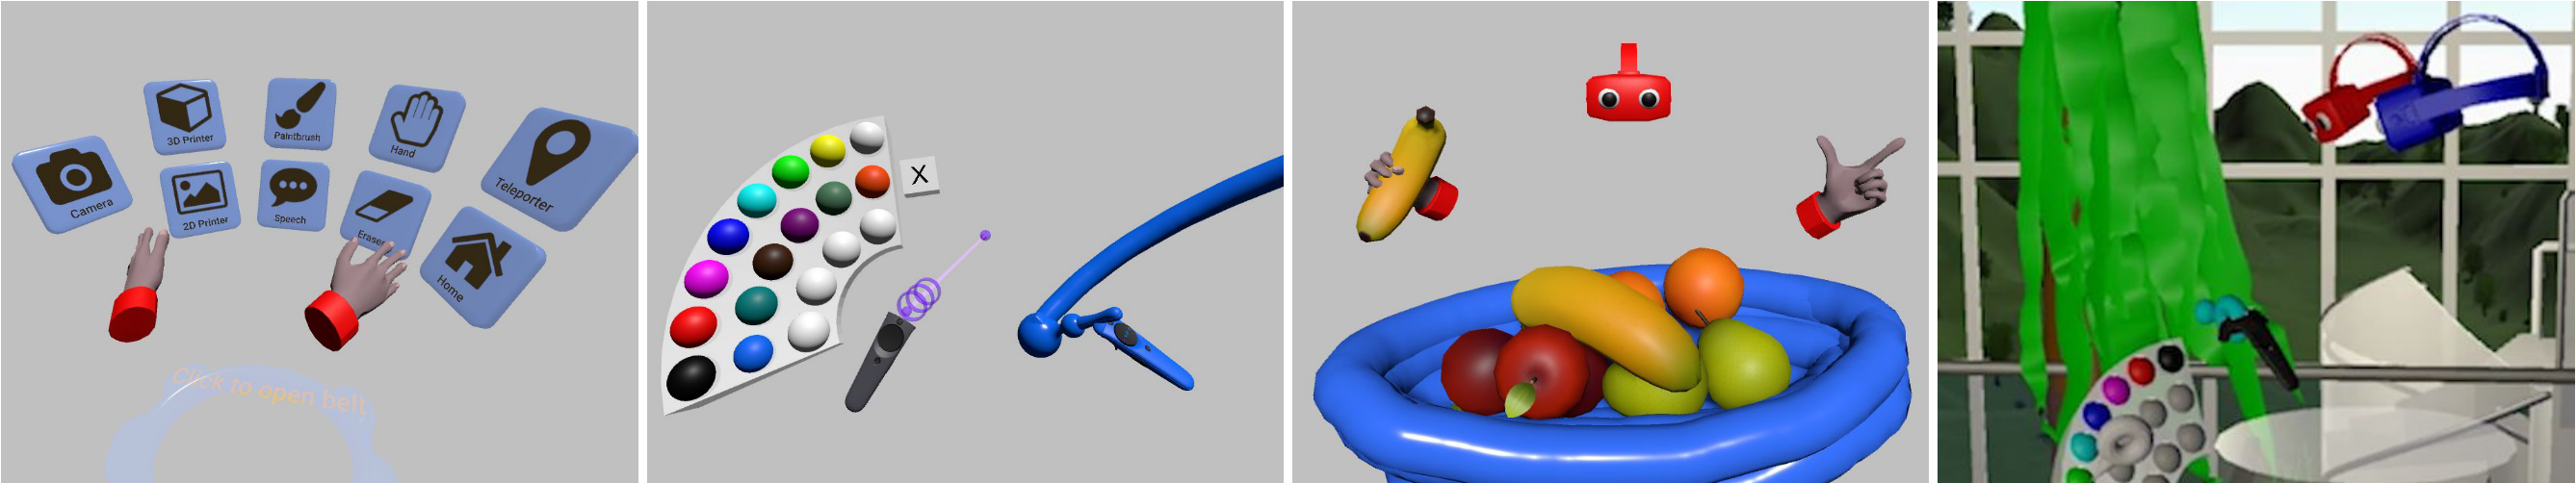
\includegraphics[width=0.7\linewidth]{figures/Cocoverse}
	\caption{CocoVerse, environment affordances and avatars (Source: \parencite{greenwald_cocoverse_nodate})}
	\label{fig:cocoverse}
\end{figure}

%% What they explored, their focus and discoveries
%%% Goals
Authors' main research direction is communication, collaboration, and learning in \gls{vr}. As the field of immersive \gls{vr} is relatively young, one of the main goals of those projects was to explore the feasibility and utility of such setup, and pilot methodologies for studying behavior in this setting (\parencite{greenwald_investigating_2017}). The utility was analyzed by comparing different activities in the 2D viewing mode (via a monitor) and as the immersive 3D experience.

%%% Setup/system
The system is a room-scale shared immersive \gls{vr} experience, which allows users to synchronously manipulate the environment with a set of hand-based tools (create 3D drawings, communicate via rough hand gestures, etc.). CocoVerse also lets the users know where others are looking, by providing them with minimalistic avatars that convey the gaze direction. Users require either a \gls{hmd} and a pair of 6 \gls{dof} controllers to use the system in the immersive mode, or simply a PC to participate in the 2D mode.

%%% Focus and the results
Authors report the overall success and promise of such setups as an engine for learning and creativity. They further review, how the sense of social presence is influenced by the complexity of avatars and high movement realism. \parencite{greenwald_investigating_2017} proposes guidelines for deciding on the level of sophistication of the embodiment based on the type of experience that is being digitalized.

% Concise: what other CVE projects addressed.
Among other CVEs that were explored, \parencite{lena_real-time_nodate} proposes a system, which connects two different mediums (an interactive table computer, and a CAVE-environment), and focuses on the way to develop consistent interactions across the environment. % TODO: more (e.g. Kulik)

% Conclusion: something else is needed
Generally, it seems that the focus of the modern \gls{cve} projects is more on exploring the aspects of the intentional communication and interactions, where users are always aware of each other during the collaboration task. I our case, the focus should be more on consequential communication, which arises as a result of user's actions.

\subparagraph[CSCW]{}
% CSCWs
We will now turn to the field of \gls{cscw}, which is regarded by \parencite{churchill_collaborative_1998} as the main way to approach the automation of the collaborative work, before the paradigm shift towards \gls{cve}s. \gls{cscw} applications also provide distributed access to a shared context. However, unlike \gls{cve}s, these applications provide a less malleable environment that is restricted by requirements of a certain workflow. Examples of \gls{cscw} applications include: emailing software, project management and conferencing tools, shared calendars and drawing tools, etc.

% Chalkboard, Gutwin
A notable work from the field of \gls{cscw} is the study presented in \parencite{gutwin_chalk_2011}. The authors study the use of auditory cues to promote the up-to-the-moment understanding of another person’s interaction with the shared chalkboard application, or as they call it, the "Workspace Awareness" (WA) \parencite{gutwin_descriptive_2002}. % TODO: I use the same quote in the Awareness chapter. Change.

%% What they explored, their focus and discoveries
%%% Goals
Two main goals of the study were to figure out "How much information can sound convey?" and the effectiveness of audio awareness in a \gls{cscw} application.

%%% Setup/system
The system is a 2D shared drawing application with one real (participant) and one simulated user (called an \textit{agent} in the \gls{cve} terminology). The participant has two tasks, primary and secondary. The primary task was to trace a given 2D shape (Fig. \ref{fig:gutwinchalk2011}), and the secondary was to keep track of what is happening in the shared workspace. When a participant and the agent drew, the system would emit a spatialized sound of chalk writing on a chalkboard (at a lower volume for the participant's actions). An additional way to monitor the shared environment, or as authors call it - a type of awareness presentation, was a minimap (what authors call a \textit{radar}), which showed the complete environment and the local chunk a participant was working in (indicated with a blue rectangle on the minimap).
% The workspace is seen in the figure
% Different awareness presentations - auditory and minimap
% Varying difficulty of the tracing shape

\begin{figure}
	\centering
	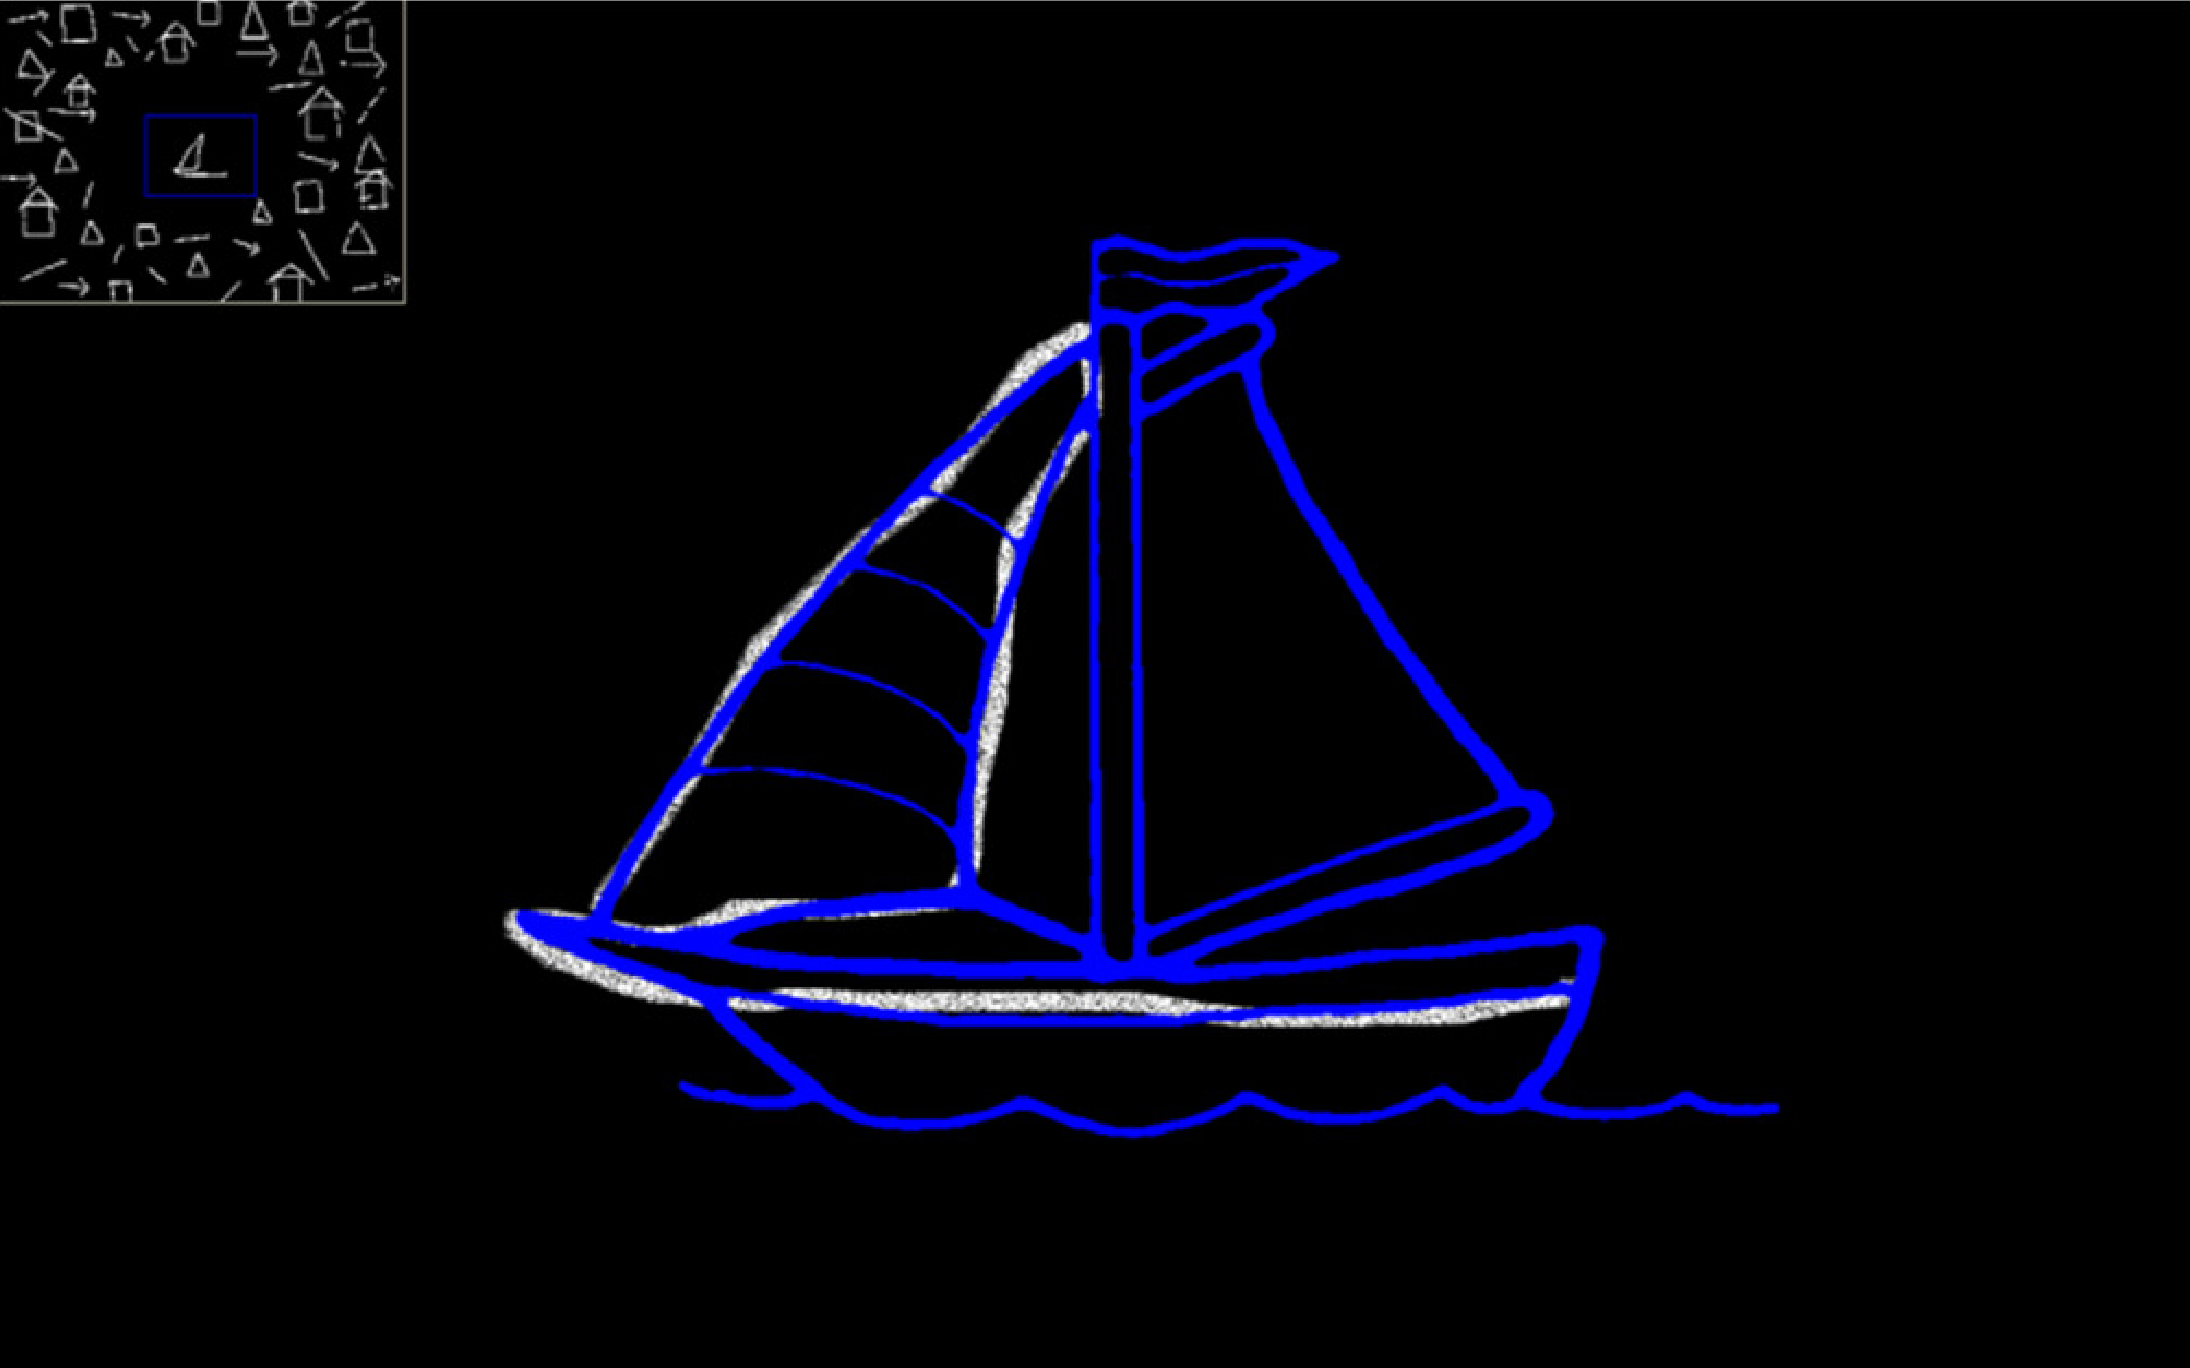
\includegraphics[width=0.7\linewidth]{figures/gutwin_chalk_2011}
	\caption{Shared chalkboard application, tracing shape and minimap (Source: \parencite{gutwin_chalk_2011})}
	\label{fig:gutwinchalk2011}
\end{figure}


%%% Focus and the results
One of the characteristics of the \gls{wa} is that it is a peripheral (or a secondary) task by nature \parencite{gutwin_descriptive_2002}, % TODO: I might be using the same quote in the Awareness chapter. Change.
as such, \parencite{gutwin_chalk_2011} attempt to keep participant's attention on the main task by varying the difficulty of the tracing activity: the tracing shape was made to oscilate occasionally. Authors also study the effect of the workspace clutter, the size of the minimap, the type of auditory cues, and the awareness presentation on the \gls{wa}.

The authors report significant improvements to the group awareness in cases, where it is hard to attend to the visual displays, or the line of sight is obscured. Additionally, they provide their thoughts with regards to how and why the audio awareness helps in the collaborative scenarios, as well as the possible limitations of its application.

\paragraph[Bridge]{}
The approach used in \parencite{gutwin_chalk_2011} is based on their previous work on the topic of \gls{wa} \parencite{gutwin_descriptive_2002}.
Next, we are going to take a closer look at the awareness approach % TODO: did I define it?
, its history, and how it aids the design of the groupware systems. 


\end{comment}





\begin{comment}
% Intro: Introduce what this whole chapter is about

This chapter is going describe the ?status quo of the Collaborative Virtual Environments, highlight the state of art, and the experiment on the Workspace Awareness that the practical part of this thesis took as the base.

\section{Status quo}
.. Like theory part
Define CVE, Groupware, and cooperation levels
% Talk about users and agents, cause I mention it in the experminets chapter.

\section{Related projects}
Mention some projects that are related, but won't be discussed in the detail in this work. The purpose of this subsection is to provide an overview of the current state of the groupware/collaborative software systems.
Lena
® Provides a good overview of the Collaboration and interaction in similar projects
® Focuses more on interactions …
Greenspace II
® A related work from the architectural filed
® Morally aged, Greenwald uses some findings from it
[some other works]

\section{State of art: Multi-User Framework for Collaboration and Co-Creation in Virtual Reality}
§ In this section I will discuss the work I found, which serves as the state of art for current development of Collaborative Virtual Environments (CVEs) - Multi-User Framework for Collaboration and Co-Creation in Virtual Reality (Greenwald et al. 2017).


\section{Parent/precursor/foundation work: The Effects of Dynamic Synthesized Audio on Workspace Awareness in Distributed Groupware}
§ Introduce Gutwin et al. 2011 work on The Effects of Dynamic Synthesized Audio on Workspace Awareness in Distributed Groupware (Chalk Sounds)

Goals

Setup/system
® …
® 

\begin{table}[]
	\begin{tabular}{|l|l|}
		\hline
		Number of people                                                                                  & Conceptually, multiuser                                                                                                \\ \hline
		Medium                                                                                            & PC with an interactive display for drawing                                                                             \\ \hline
		\begin{tabular}[c]{@{}l@{}}Affordances \\ (TODO: make it correspond to WA framework)\end{tabular} & \begin{tabular}[c]{@{}l@{}}Manipulation: 2D drawing, self-report\\ Communication: auditory icons, minimap\end{tabular} \\ \hline
		?Cooperation level                                                                                & Conceptually, 3.2                                                                                                      \\ \hline
		Locality                                                                                          & Shared physical space and remote collaboration                                                                         \\ \hline
	\end{tabular}
\end{table}

Focus and the results
\end{comment}

\glsresetall
\chapter{Properties and Applications of Audio}

% The study of sound effects dates back to bbc-years book
The use of sound effects has a long history, already in 1931 certain sound effects were used for their evocative ability to bringing up strong memories, images, or feelings in the mind \parencite{bbc_yearbook_1931}.

% Theory from earcons and icons, as the base building blocks for sound feedback

\section{Properties} 
I will start by introducing the the basic attributes of sound, which will be helpful for the further discussion. First of all, sound are audible waves of pressure traveling trough a medium, and emitted by a vibrating object. The range of audible frequencies depends on the species, for humans it is usually 20 Hz to 20 kHz. Frequency of the sound defines its pitch, higher and lower pitch correspond to higher and lower frequency, respectively. A tone is a sound with a certain pitch The lowest frequency of a vibrating object is called the fundamental frequency (indicated as f; Fig. \ref{fig:fundamentalfrequencyandharmonics}). Its positive integer multiples are called harmonics (indicated as 2f, 3f, and so on). The fundamental frequency is also called the first harmonic. Pressure waves with higher frequency than that of the first harmonic, but not its positive integer multiples, are called overtones. A musical tone (a steady periodic sound) can have the same fundamental frequency, duration, and loudness, as another tone, but have a different feel. For example, consider the same melody played by a banjo and a guitar. They will feel differently due to an attribute called timbre (or tone color) \parencite{noauthor_fundamental_nodate}. \parencite{blattner_earcons_1989} write: "the timbre of a sound is usually described with adjectives such as bright, warm, harsh, hollow, twangy, or brassy". A sound that comprises of one sine wave, only its fundamental frequency, is timbreless, "the sine wave lacks timbre in the same sense that white lacks color" \parencite{blattner_earcons_1989}.

\begin{figure}
	\centering
	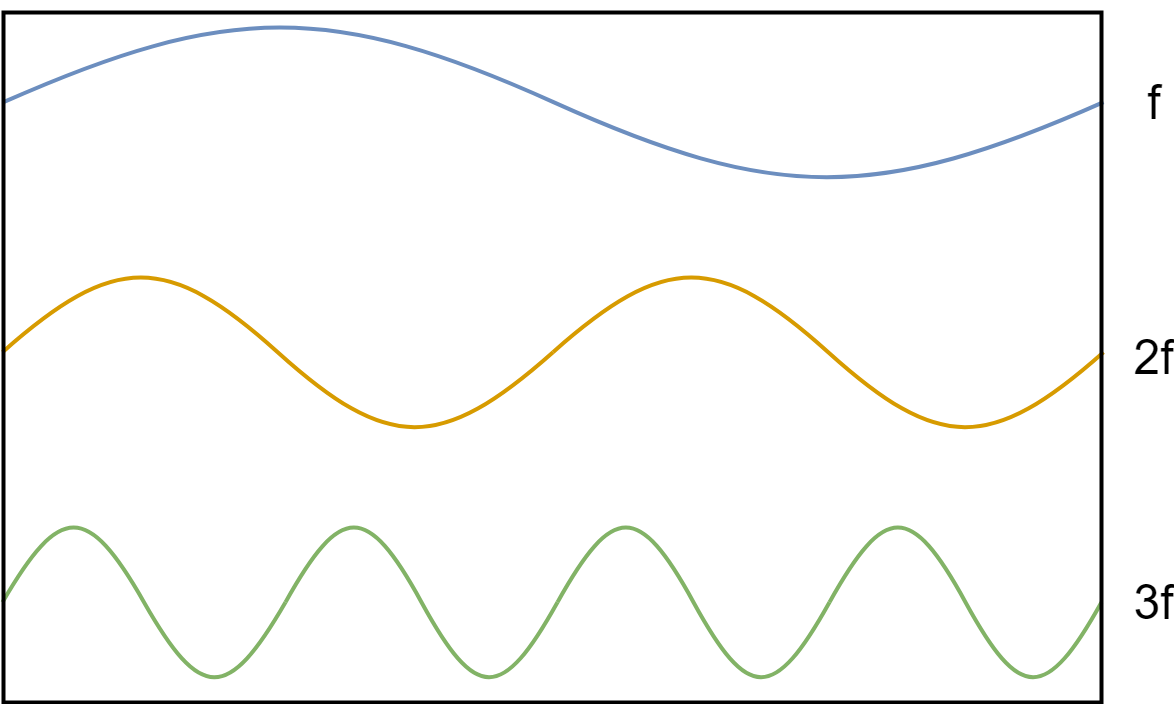
\includegraphics[width=0.7\linewidth]{figures/fundamental_frequency_and_harmonics}
	\caption{Fundamental frequency and its 2nd and 3rd harmonics}
	\label{fig:fundamentalfrequencyandharmonics}
\end{figure}

\parencite[p.~46]{jr_3d_2017} argue that the auditory sensory system is the second-most used sensory channel after the visual channel . As with the visual system, the auditory system provides us with different localization cues that allow us to determine the direction the sound is coming from and distance to it. The main types of \textit{auditory cues }are:
\begin{description}
	\item[binaural cues] - the direction of the sound source is derived through comparing the sound waves received at each individual ear. The limitation of binaural cues is that there are certain positions around the listener, where the cues are ambiguous and it is not possible to uniquely identify the direction;
	\item[Head-Related Transfer Functions (HRTFs)] - spatial filters that are applied to the original sound when it goes through the listener's torso, shoulders, head, and the outter ears. The latter contain different notches and grooves that elevate of suppress sound depending on which direction it came from. HRTFs help solve ambiguous cases caused by binaural cues;
	\item[reverberation] - the collection reflected sound waves from the surfaces in the environment. Besides providing the listener with spacial information about the layout of the environment, reverberation allows them to determine the distance to the sound source;
	\item[sound intensity] (loudness) - the primary cue in determining the sound source's distance. It is also a very simple cue to implement.
\end{description}
The authors also note that auditory cues combined with visual cues can be used to form better spatial perception of the environment. Additionally, the familiarity with the environment can influence the listener's ability to locate the sound source.

Another important aspect for presenting the aural information to the listener is the selection of an \textit{auditory display} \parencite[p.~153]{jr_3d_2017}. It defines the way in which audio is synthesized, how it is presented to the listener, and the ways in which audio feedback are used in the application.
Different approaches to audio synthesis (i.e. using mathematical models, or sound sampling) have direct influence on the resulting auditory cues. For example, in case of taking HRTF measurements during sound sampling, this is usually done in echo-free environments, therefore, the recorded sound is stripped of the reverberation effect. This influences the perception of distance to the sound source

The authors point out several different ways in which audio displays can be used:
\begin{description}
	\item[localization] determining the direction and location of a sound;
	\item[sonification] turning information into sounds;
	\item[ambient effects] adding realism and the sense of immersion in a 3D application;
	\item[sensory substitution] playing a role of another perceptual cues (i.e. emitting a sound instead of haptic feedback); 
	\item[annotation and help] providing additional guidance in the environment (i.e. recording vocally indicating the correct way, or the auditory annotations of a previous user about an artifact in the shared environment).
\end{description}

\section{Sonification for Monitoring}
\parencite{hermann_sonification_2011} argue that sonification has great application in monitoring. While it might seem to be a part of the localization task, cognition is also required for monitoring, not just perception of the sound source - users must understand what the emitted sound conveys.

% Monitoring
One of the problems with auditory displays is that they are a temporary medium, that is - not available for immediate review at any given time. The authors argue that this is the exact reason that makes auditory display a perfect match for the monitoring task, as it is often carried out as a secondary task in parallel with one or more primary tasks, and is based on paying attention to the temporally-related changes to the state of the system.

% Types of monitoring
Monitoring can be classified into two types: \textit{information pull} (\textit{direct monitoring}) and \textit{push}. The former is the case, when monitoring is a primary task and is attended by the user intentionally, the latter treats it as a secondary task, and therefore the information has to be "pushed" into the user's attention space. The push category can be additionally substituted into \textit{peripheral} and \textit{serendipitous-peripheral monitoring}, depending on the role the information plays for the primary task: important or just a convenience (serendipitous) role, respectively.

% Modes of listening
Human hearing can also be classified in several different ways. If we use the push and pull analogy, \textit{hearing is a push} activity, where sounds are forced onto the listener, and \textit{listening is a pull}, where the listener is intentionally attending to the information being conveyed through sound \parencite{hermann_sonification_2011}. Other classifications categorize listening based on the attention to different properties of sound. In this way, \textit{everyday} (or \textit{casual}) \textit{listening} refers to the activity, where attributes of the sound source are being attended: "\textit{big} lorries, \textit{small }children, \textit{plastic }cups being dropped, \textit{glass }bottles breaking", etc. On the other hand, in \textit{musical} (or \textit{reduced}) \textbf{listening}, humans attend to the attributes of the sound (pitch, intensity, timbre, and so on). \textit{Semantic listening} mode involves interpretation of the message encoded in the sound. In this way, the same vocal message with different "muscial" properties can be interpreter equally.

% Some interesting systems (AR-Kola)
% ...

% Pitfalls - annoyence and stuff
There is a number of pitfalls when designing auditory displays, most of them can be classified into either \textit{intrusion and distraction, fatigue and annoyance}, or \textit{audience related sonification problems}.
% intrusion and distraction, fatigue and annoyance
The former mainly explores the trade-off between intrusiveness of the sound and the communicating enough information. \parencite{hermann_sonification_2011} reviews the different ways that were previously employed in an attempt to tackle this problem. For example, sounds that fit to the working environment ecologically, like ticking clock in the office environment, can be less intrusive due to the fact that they correspond to the listener's expectations of the environment. However, non-intrusive sounds lose their perceived importance for the listener. To tackle this problem, the minimal intrusion can be intentionally imposed by variable speed, timbre, or intensity of sound to simultaneously draw listener's attention, and not obstruct the work too much.

%% Audience based: emotional associations, auesthetic and acoustic ecology (allowing users to choose the ecology), and comprehesibility and audibility.
There can be different audience related sonification problems, \parencite{hermann_sonification_2011} reviews three: \textit{emotive associations}, \textit{aesthetic and acoustic ecology}, and \textit{comprehensiveness and audibility}. Different users require different information from the data, and emotive association accounts for that. It describes the problem of presenting information that is too detailed to the parties that do not need it (i.e. sonification of the weather reports for meteorologists and average consumers should be yield different results). Aesthetic and acoustic ecology corresponds to the idea of combining compatible sounds in an auditory display (in terms of frequency and intensity balance, correspond to the same theme, and take the cultural and personal differences of the audience into account. Comprehensiveness and audibility of auditory cues can be highly dependent on the social and cultural norms, and therefore have to be designed with the listener target group in mind.

\paragraph[]{Earcons and auditory icons}
The last topic I will review in this chapter concerns different ways of sonifying information. \parencite{blattner_earcons_1989} review earcons, the aural analogy of a visual icon (i.e. desktop icons in Windows or Mac OS), and divide them into three groups, in alignment with previous research on the visual icons: \textit{representational}, \textit{abstract}, and \textit{semi-abstract earcons}. 
The difference between the three classes is reflected in their names:
\begin{description}
	\item[representational earcons] rely on digitalization of the natural sounds and their mainly metaphoric use in the computer systems (i.e. sound of a tap with your finger as a sound of clicking on a folder);
	
	\item[abstract earcons] rely on the notion of "elements" (the short (abstract) sound blocks) that can be combined into structures (i.e. a tree) to explain the relationship between some actions (see Fig. \ref{fig:iconstreestructure} for an analogy of element with hierarchical icons);
	
	\item[semi-abstract earcons] are a combination of the previous two classes.
\end{description}

\begin{figure}
	\centering
	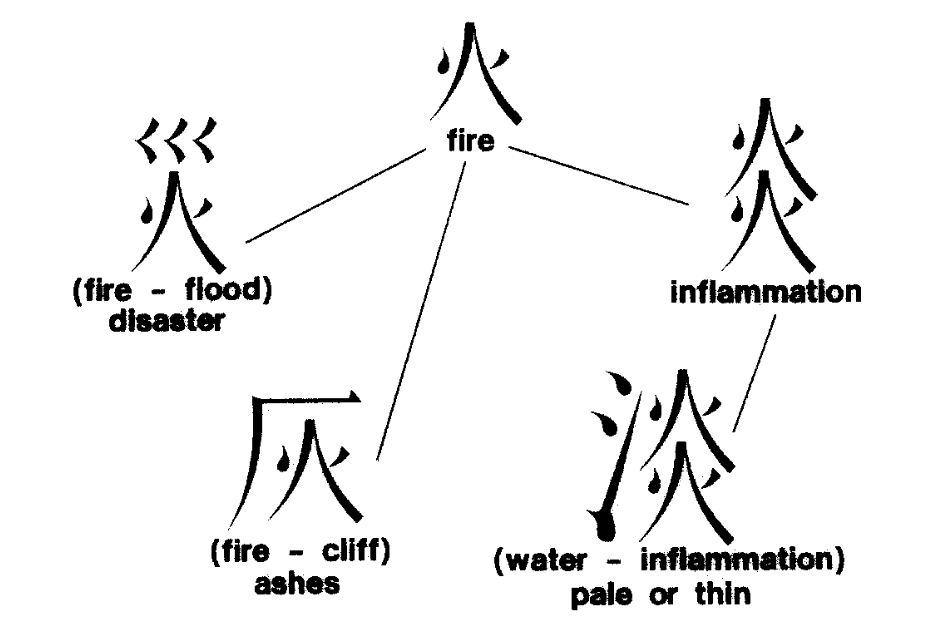
\includegraphics[width=0.5\linewidth]{figures/placeholders/icons_tree_structure}
	\caption{Hierarchically abstract icons. Source: \parencite{blattner_1989_earcons}}
	\label{fig:iconstreestructure}
\end{figure}

There is no clearly superior choice. \parencite{gaver_sonicfinder:_1989} addresses representational earcons as \textit{auditory icons} and argues that this approach brings implicit benefits by exploiting the natural way we as humans react to sound. 
However, \parencite{blattner_earcons_1989} conclude that even though auditory icons are easily distinguishable and mappable, the main benefits of their application would be in systems with few distinct sounds: for $n$ different events $n$ mappings have to be memorized.
On the other hand, abstract earcons, while baring no intuitive relation to the event, require less mappings to be memorized due to their modularity: for $n$ different events, where $pq=n$, and $p$ and $q$ are distinct, unrelated elements, $p+q$ mappings have to be memorized.
% TODO: additionally, auditory icons need to be in their original ecology, and even then the mapping has to be learned. Even though that would be slightly more intuitive than learning abstract earcons.

\paragraph[Bridge]{}
Having reviewed the sound-related topics, which are relevant at the perception stage, it is time to take a look at the cognition stage of the information processing loop.
% TODO: situation awareness, actually, resides in both perception and cognition stages.


\begin{comment}
%(really small chapter, explaining the possible ways to implement auditory cues [auditory icons, earcons, …])

% Reference list
%% The Sonification Handbook

%% Sandell Kramer's book review
Sonification - The citation "non-speech audio to convey or perceptualize data"
%% Blattner. Earcons and icons

%% ? 3D User Interfaces

%% ? Kronland-Martinet, Real-time perceptial simulation of moving..

%% BBC Year Book
"The Symbolic, Evocative [bringing strong memories, images, or feeling to mind] Effect; e.g. the churning rhythm record used to express the confusion of a charwoman's mind in "Intimate Snapshots "; the use of sea sounds between all scenes in "The Flowers are not for You to Pick," expressing the inevitability of disaster."
%% Sound Immersion in First-Person Shooter


% TODO: also cite Gutwin 2002: the pre-research and the findings (the limitations of audio awareness, and "How and why does audio improve awareness?")
% TODO: maybe cite Gutwin 2011, too. THere was something on sound being a good tool or wharevs

Previous chapters implicitly established that auditory cues could potentially be a great way for providing awareness about the workspace. In this chapter I review sonification and the means it provides us with that can be utilized for interpretation of certain events or data. Sonification is a concept akin to visualization. Both can be applied to data, and while the visualization will do it in a visual form, sonification will use "non-speech audio to convey or perceptualize data".

\section{Sound Properties}
% I mention timbre in Experiments chapter
% + harmonics & halftones (and how they allow to differentiate between sounds), fundamental frequency
% Occlusion in audio SDKs
% 

% TODO: explain them here, but use as an example in later chapters. Potentially, like the chapter before
% HRTFs and stuff? Can tie the stereo headphones here as a exapmle of why they suck.

	
\section{Auditory Icons}
\section{Earcons}
\section{Summary}

Bridge: In the next chapter we will combine the knowledge from the previous chapters to …

\end{comment}
\glsresetall
% !TeX root = ../main.tex
% Add the above to each chapter to make compiling the PDF easier in some editors.

\chapter{Awareness}

This chapter is going to introduce \gls{wa}, as a tool for developing productive collaboration systems. We will start by looking at the \gls{sa}, as it serves as the theoretical foundation that the concept of \gls{wa} builds upon.

\section{Situation Awareness}
% This section serves as a pre-cursor to the Workspace Awareness section, and shows the base that WA is built upon.

%Situation awareness itself
\gls{sa} is usually used in attention-critical and hazardous tasks, where failure to react to the a change in a system might cause serious and even lethal consequences. SA served as one of the base notions, on which the concept of the workspace awareness was built.

\gls{sa} has seen great development through its application in the aviation field, and \cite{endsley_situation_1988} defines it as a combination of: perception of the elements in the certain volume around the user at the given time; comprehension of the meaning of these elements; and the ability to project their state into the nearest future.

[Not finished. TODO: More info from \cite{endsley_situation_1988} (human factors, levels of awareness, etc.)]
%* Write about the jet fighter simulator somewhere
%o Human factors?
%o Levels of awareness // <- I will classify my system according to this in the end

\paragraph{Measurement}
\cite[p.~791-792]{endsley_situation_1988} reviews different approaches to the measurement of \gls{sa} that help system designers answer the fundamental question: "Does system A promote better SA than system B?". In the author's opinion, all the approaches that were available up to that point suffer from their own individual limitations. For example, the subjective approach, where the subject is asked to rate his \gls{sa} from 1 to 10 suffers from 2 major drawbacks: first, the subject is not aware of "what is really going on in the environment", and secondly, the outcome of the task can influence the rating. Similarly, the psychological approach suffers from the incomplete human-computer interfaces to monitor what is going on with the pilot at this moment, and what they are thinking about. Finally, if the questionnaires are used, the fact that humans are not that good at recalling past mental events comes into play. Another set of problems arises, if an attempt is made to solve the issue with the questionnaire approach by querying pilots in real-time, such as the pilots can start to attend to the information they are questioned upon more thoroughly or they can be under a heavy load at the moment of questioning, which would obstruct their answer.

Nevertheless, \cite{endsley_situation_1988} finds the biggest limitation of the mentioned approaches was that they attempted to evaluate only a single design issue at the time. All this leads \cite{endsley_situation_1988} to introduce the \gls{sagat}. The idea here is that, first, the task goes though goal-directed analysis to determine the \gls{sa} requirements: the goal, subgoals, decisions required to actualize the given subgoal, and the knowledge required on all three levels of \gls{sa} (\ref{fig:sagoalorientedtaskanalysis}). 
\begin{figure}
	\centering
	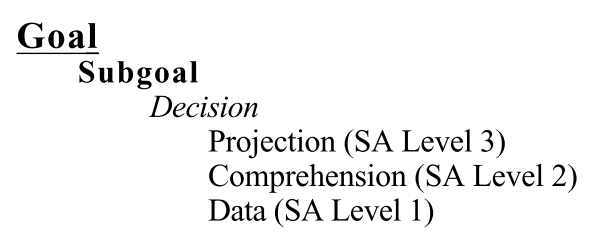
\includegraphics[width=0.7\linewidth]{figures/placeholders/SA_goal_oriented_task_analysis}
	\caption{Format of Goal-Directed Task Analysis (totaly spizgenoe name from: \cite{endsley_direct_nodate})}
	\label{fig:sagoalorientedtaskanalysis}
\end{figure}
This should yield an extensive list of questions, which assess SA information the \gls{sa} information of primary and secondary importance (for an example of the results of such analysis, see the Fig. \ref{fig:sagoalorientedtaskanalysisresultexample}).
\begin{figure}
	\centering
	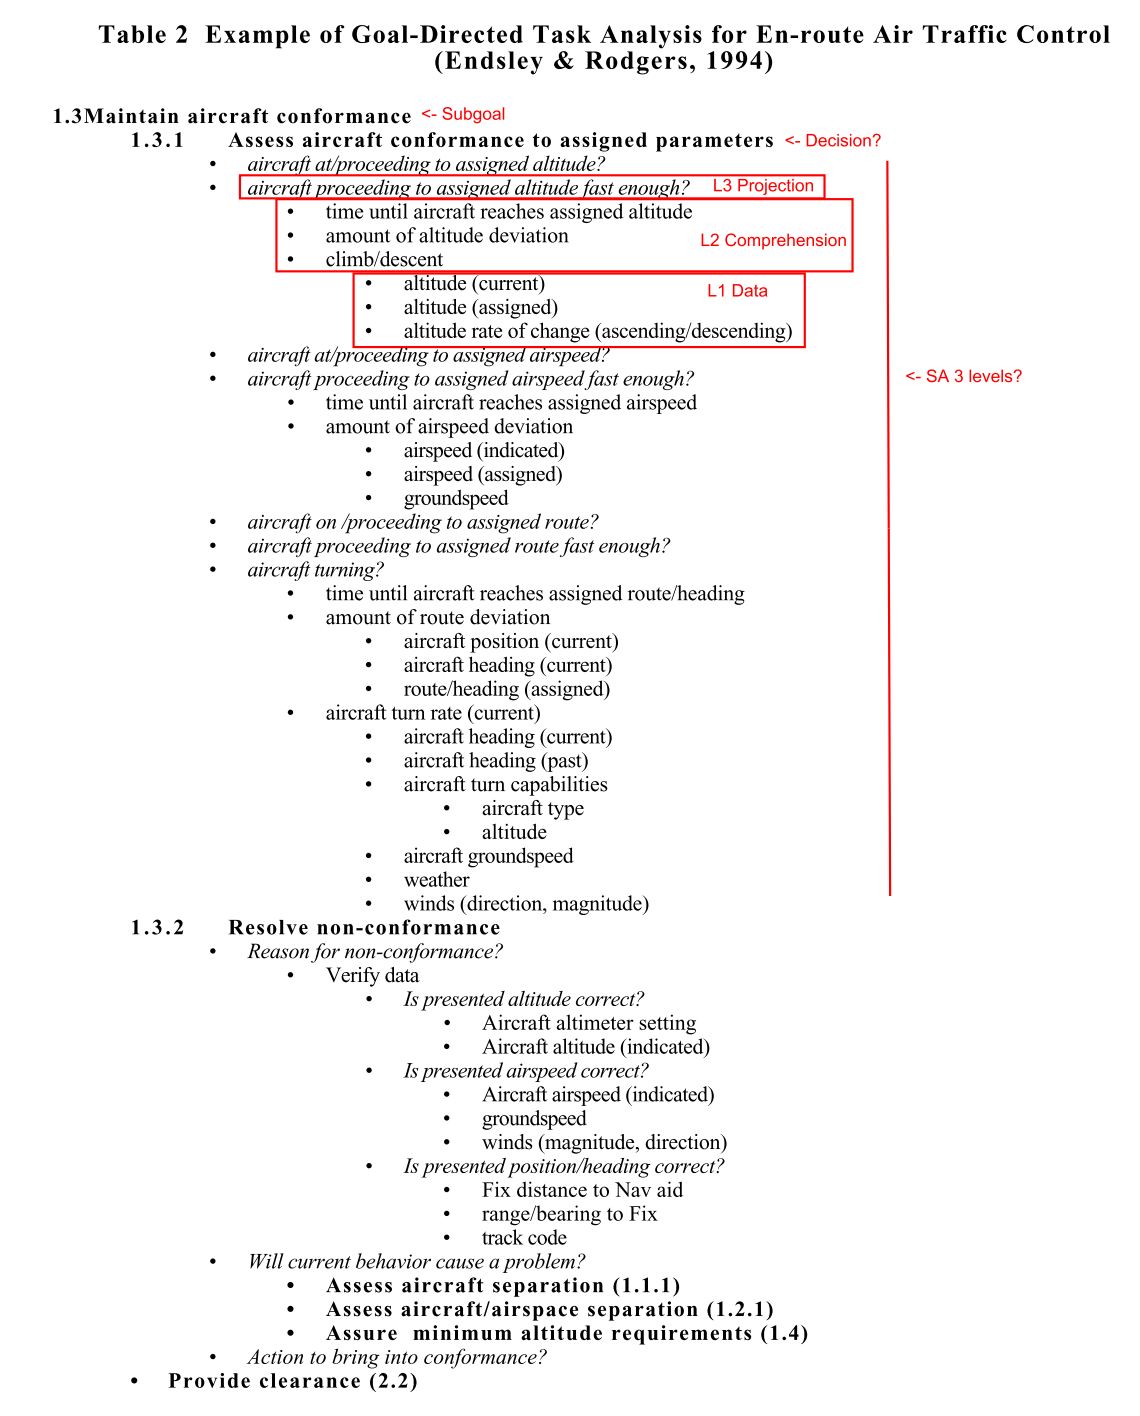
\includegraphics[width=0.7\linewidth]{figures/placeholders/SA_goal_oriented_task_analysis_result_example}
	\caption{Example of Goal-Directed Task Analysis for En-route Air Traffic Control (Endsley \& Rodgers, 1994) [from: \cite{endsley_direct_nodate}]}
	\label{fig:sagoalorientedtaskanalysisresultexample}
\end{figure}
Next, at some point in time, the simulation is halted, and the pilots are queried on the randomly selected questions from the list. When the simulation halts, all the control panels, the ?windshield of the jet-fighter, and other simulation elements are grayed-out. Not every pilot is queried on every question, the goal is to reach the desired statistical significance of the results by assessing a certain number of participants.

% This paragraph is a bit repetetive
By using this approach, it is possible to get a snapshot of the current situation in the point of view of the pilot, which is unbiased by the recall difficulties, and that can be compared to the actual situation after the experiment. Additionally, pilots' \gls{sa} is not artificially enhanced, because the questions do not always directly address the main goals in the current situation, but can concern secondary information, which is still relevant.

\cite{endsley_direct_nodate} notes that, since the introduction of \gls{sagat}, there is practical evidence that the method is valid, reliable, non-intrusive (in case of the halts are made at unpredictable time points), and is able to properly "reliably tap into memory stores" acting as a \gls{sa} index. 


o Bridge to Workspace Awareness


\section{Workspace Awareness}
% Definition
\gls{wa} can be described as "the up-to-the-moment understanding of another person’s interaction with the shared workspace" \cite{gutwin_descriptive_2002}. While this is a trivial task in real-world face-to-face collaboration, \gls{wa} becomes a bottleneck for productive collaboration because of limited information that systems usually provide, and unfamiliar interaction interfaces.
 
% Description
It is an extension of the concept of \gls{sa}, research from the \gls{hci} and \gls{cscw} fields, and authors' own observations and research. \gls{wa} could be characterized as an adaptation of \gls{sa} to the day-to-day working scenarios. This was desired, because as authors put it: "sorting slides on a table does not seem very similar to air combat in a jet fighter" \cite{gutwin_descriptive_2002}, or in our case, to architectural collaboration in immersive \gls{vr} environment. Another major difference of \gls{sa} and \gls{wa} is that besides maintaining their \gls{sa} and performing the domain (their personal) task, collaborators have to perform their collaboration.

% Framework 'classification'
This led \cite{gutwin_descriptive_2002} to develop the \gls{wa} framework, which concerns itself with providing a toolset for describing and analyzing medium-sized workspaces. The framework is applicable to real-time distributed groupware for shared environments, and small mixed-focus collaboration groups busy with generation and execution tasks.
% Framework descriprion
The \gls{wa} framework is split in 3 parts: "What information makes up \gls{wa}?", "How is \gls{wa} information gathered?", "How is \gls{wa} used in collaboration?". 
In Part I the authors address the information that collaborators might require from the workspace. While this can be any type of information, it can be categorized into the most common types. For example, the category "Who" concerns itself with the presence, identity, and authorship questions, and contains the following questions: "Is anyone else in the workspace?", "Who is participating? Who is that?", and "Who is doing that?". An example for the "Who" category can be seen in Fig. \ref{fig:watechniquesforwhoquestions}. There are 8 categories of questions in Part I of the framework: questions about the present (Who?, What?, Where?), and questions about the past (How?, When?, Who? (past), Where? (past), What? (past)). The \gls{wa} framework doesn't concern itself with the information about the future, because this requires projection.
This part of the framework allows designers to compare and design awareness support in different groupware applications by providing a fixed vocabulary for describing their systems.
Part II of the framework deals with the ways the information can be delivered to the users. The authors present 3 ways in which the information can be communicated in a workspace: through bodies and consequential communication, through artifacts and feedthrough, and through conversation, gesture, and intentional communication. While the last one speaks for itself, the first two deal with information transfer through the consequence of people's actions in the workspace, and the information emitted by the manipulated objects in the workspace (for example, a characteristic sound initiated by a person drawing in the workspace).
By considering the different ways in which the information transfer can occur, system designers can make an educated decision about what approach to use in a particular situation.
Part III of the framework turns to the question of how we make use of the information we gather through \gls{wa}. Here we discover 5 types of activities that benefit our \gls{wa} in some way: management of coupling, simplification of communication, coordination of actions, anticipation, and assistance (see summary in Fig. \ref{fig:summaryofactivitieswherwacanbeused}).
This part of the framework allows awareness designers consider different ways people make use of the awareness information, and decide where, whether, and how much of this information is required.
For example, if we take anticipation, "People anticipate others in several ways. They can prepare for their next action in a concerted activity, they can avoid conflicts, or they can provide materials, resources, or tools before they are needed".


\begin{figure}
	\centering
	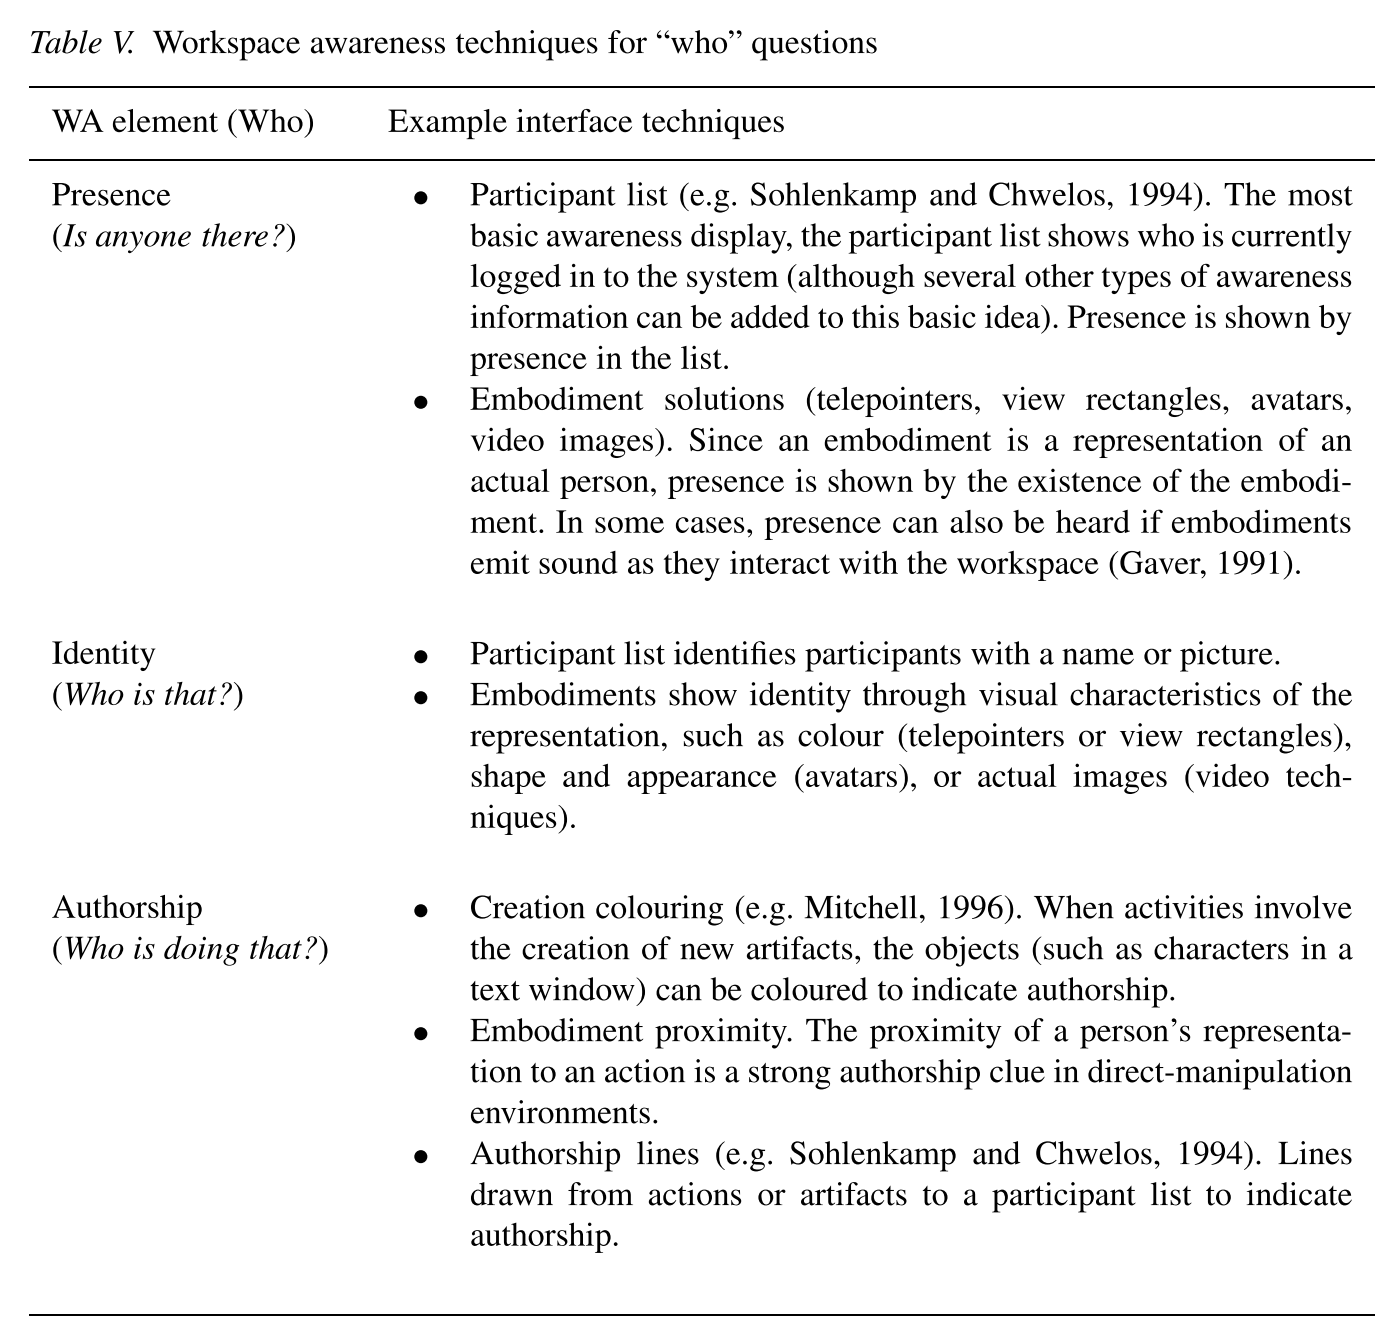
\includegraphics[width=0.7\linewidth]{figures/placeholders/WA_techniques_for_WHO_questions}
	\caption{}
	\label{fig:watechniquesforwhoquestions}
\end{figure}

\begin{figure}
	\centering
	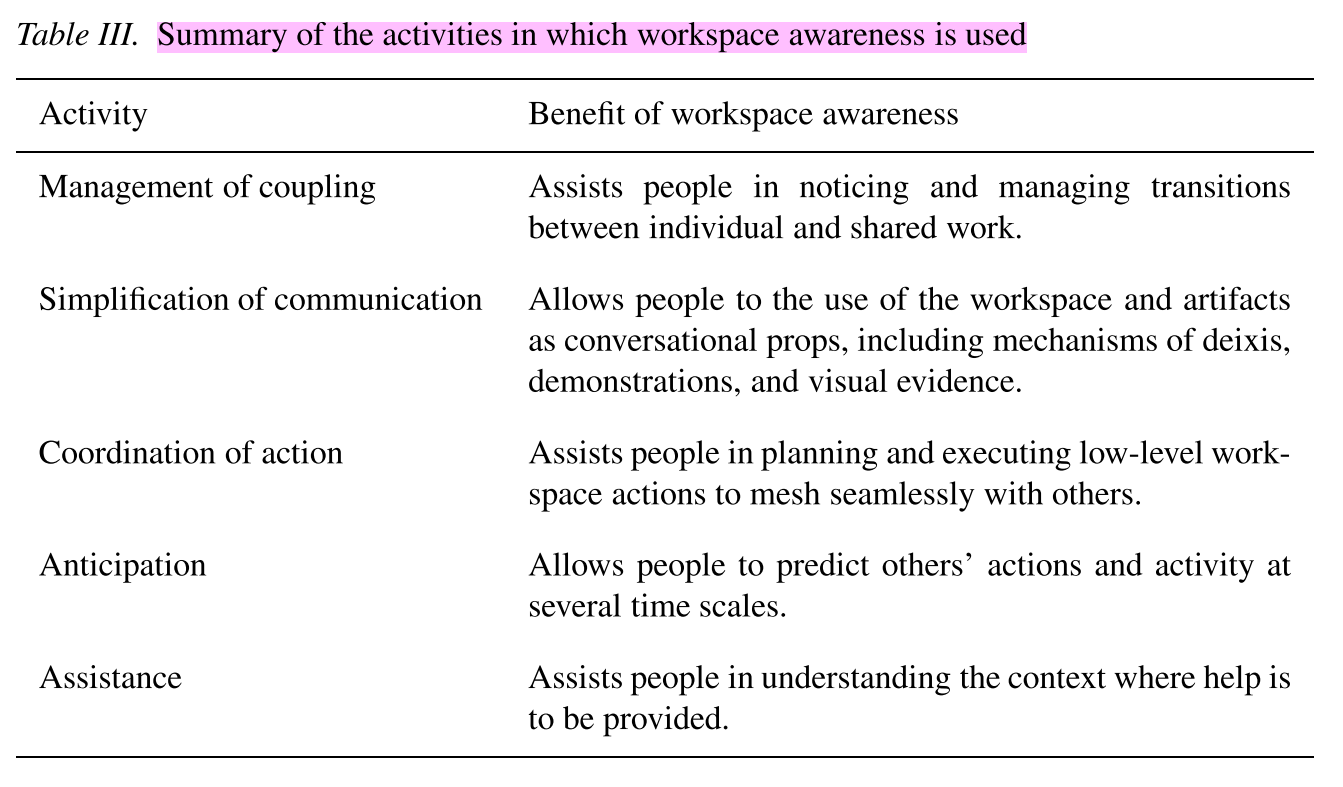
\includegraphics[width=0.7\linewidth]{figures/placeholders/summary_of_activities_wher_WA_can_be_used}
	\caption{}
	\label{fig:summaryofactivitieswherwacanbeused}
\end{figure}


The figure summarizing the framework:

\begin{figure}
	\centering
	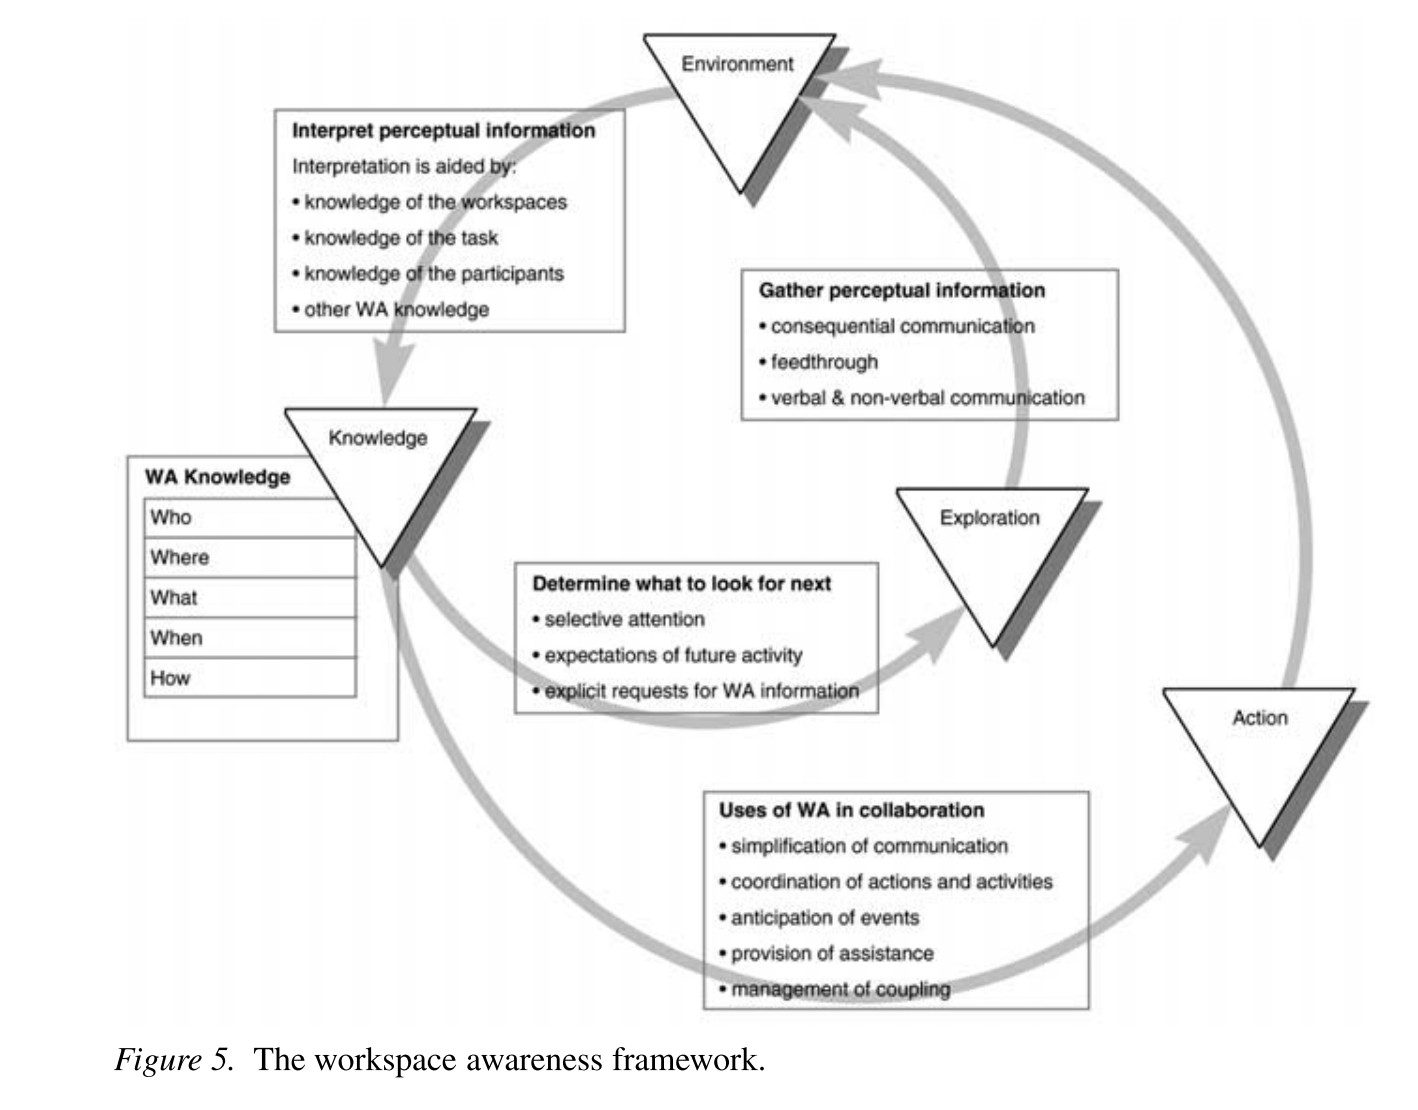
\includegraphics[width=0.7\linewidth]{figures/placeholders/WA_framework}
	\caption{}
	\label{fig:waframework}
\end{figure}


%o Relation to human factors’ research?

* Measurement
?SAGAT is sorta not applicable, because not so many elements to query upon.
o Bridge to Sonification: 
* Awareness - secondary/monitoring task \& sonification is great for monitoring -> use it for our experiment 
"Awareness is a secondary goal in the task – that is, the overall goal is not simply to maintain awareness but to complete some task in the environment"


\glsunsetall
% !TeX root = ../main.tex
% Add the above to each chapter to make compiling the PDF easier in some editors.

\chapter{Experiments}

In total, 5 experiments were conducted for this thesis. Two were quick proof-of-concept experiments to validate the initial speculation, two - pilot studies to determine values for some properties of the final experiment and test the process of sampling participants on \gls{wa} index, and one formal study to test \nameref{final_study}. 
The audio specialization tool used in all the pilots and final studies was Resonance Audio SDK for Unity with occlusion effect turned off.
Participants in all of the studies were asked for their consent, in case they were recorded.


\begin{comment}
\section{Prototypes/Proof of concept}

Initial motivation for this work was a question of whether sudden manipulations of buildings in \gls{vr} would cause uncomfortable experience for users (Fig. \ref{fig:a1unawareofa2actions}). Two prototypes were developed to test this speculation, these are described in the Buildings Popping Up and Moving Buildings paragraphs.

\begin{figure}
	\centering
	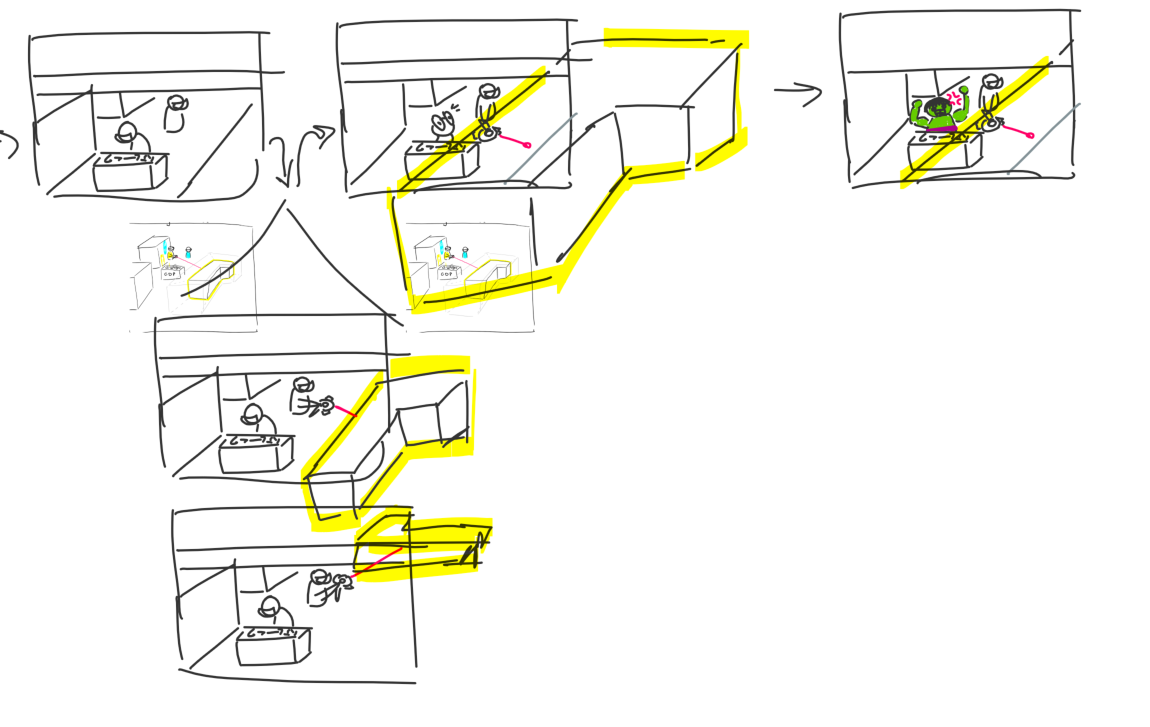
\includegraphics[width=0.7\linewidth]{figures/placeholders/A1_unaware_of_A2_actions}
	\caption{Collaborators unaware of each other's actions}
	\label{fig:a1unawareofa2actions}
\end{figure}

\paragraph{Buildings Popping Up} 
\label{buildingspoppingup}
The first prototype looked into how the participants' experience would be influenced, if a building suddenly appeared in-front of them, when they were occupied with their own task.

% Participants
3 participants (all male) were chosen among the members of the \gls{hci} group at the University of Otago. Two had prior experience in \gls{vr}, one had not.

% Procedure & Task
Participants were placed in the immersive \gls{vr} environment: a 3D model of the campus of the University of Otago. This was not a collaborative task, the participants were in the \gls{ve} alone. First, the the affordances of the environment were introduced (teleportation, walking and looking around), then participants were asked to navigate to the university clock tower. During this navigation task, a building would pop up in-front of them a couple of times at pseudo-random times (decided and initiated by the experimenter). After the completion of the experiment the participants were asked to describe the experience, especially the parts, where a building appeared in-front of them.

% Apparatus (i.e Unity, Resonance Audio, stereo headphones, Vive)
Unity3d and Oculus Rift \gls{hmd} with Touch Motion controllers were used in this experiment.

% Results
The participant with no prior experience in \gls{vr} described the experience as unexpected, but was also not sure, whether he caused it. The other two participants indicated that they were a bit stuttered by the experience, but in general, "didn't care much for it". Additionally, the participants described the experience as irritating, when the building continued to repeatedly appear after the first encounter.
% Limitations
% I do not check if anyone is concerned with the moving buildings when they get used to it.
% This doesn't matter tho, because according to the WA, people should know what the others are doing in the same environment.
% Discussion of the results?
%...


\paragraph{Moving Buildings}
Due to the results of the first experiment, the problem was regarded as worthwhile of further exploration. For the second proof of concept, a decision was made to come a bit closer to the initial motivation: buildings moving in \gls{ve}.
% Participants
4 new participant (all male) were chosen among the members of \gls{hci} group at the University of Otago, none took part in the previous experiment. Three had moderate experience with \gls{vr}, one had little.
% Procedure & Task
The environment affordances and the introduction remained the same. The task was extended, so that when participants find the clock tower, they were asked to assume their place at the viewing spot prepared for them (Fig. \ref{fig:prototype2viewvingspot}). At this point the participants were asked to observe the clock tower and tell the experimenter if anything seemed odd about it. Some elements of the tower were off axis (Fig. \ref{fig:prototype2clocktoweroddfeatures}), and this task was meant to lull participants' vigilance. As soon as participants started looking for any odd features, the movement of the clock tower towards the used with the speed of 200 units (meters) per second was initiated by the experimented. The approximate distance to from the viewing spot to the tower was 69 meters, the clock tower would stop 0.5 meters in-front of a participant. At this point the experiment would finish, and the participants would be asked about their experience.
\begin{figure}
	\centering
	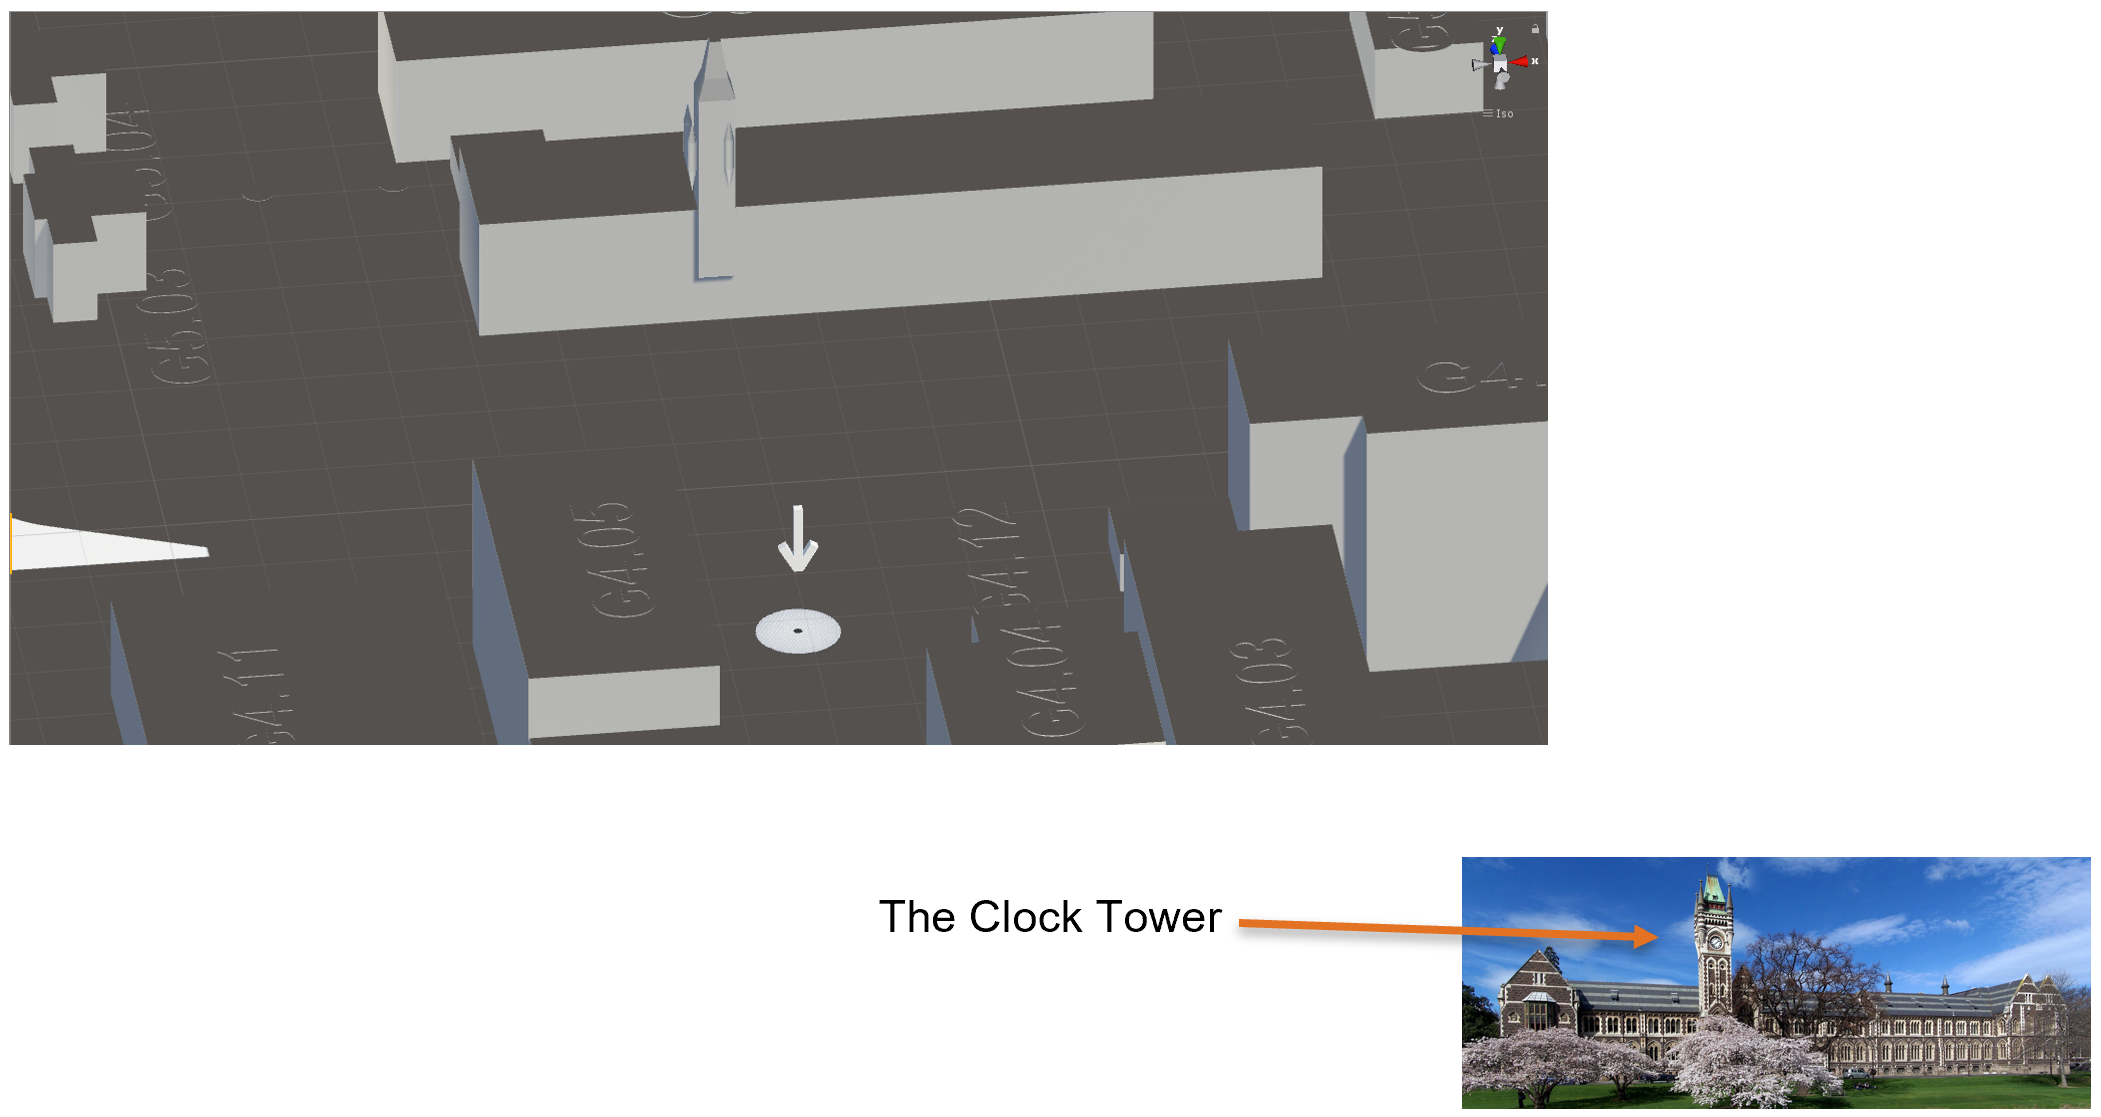
\includegraphics[width=0.7\linewidth]{figures/placeholders/prototype2_viewving_spot}
	\caption{The viewing spot in-front of the university clock tower}
	\label{fig:prototype2viewvingspot}
\end{figure}
\begin{figure}
	\centering
	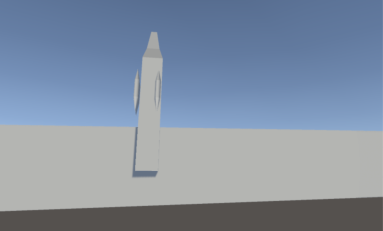
\includegraphics[width=0.7\linewidth]{figures/placeholders/prototype2_clocktower_odd_features}
	\caption{The odd features of the university clock tower model}
	\label{fig:prototype2clocktoweroddfeatures}
\end{figure}
% Apparatus
The same apparatus was used, as in the \nameref{buildingspoppingup} prototype.
% Results

% Limitations
\end{comment}


\section{Pilot Studies}
In preparation to the \nameref{final_study} study, two pilot studies were conducted: \nameref{study_one}, and \nameref{study_two}. This was done to study certain aspects of the final study separately, and make decisions, such as what sound type (earcons or auditory icons) to choose, and at what speed to translate the buildings.
















\subsection{Sound Speed and Type}
\label{study_one}
% Goal of the study
Some feedback from the initial prototypes indicated that the speed of the moving building was either too fast, or too slow. The goal of this study was to derive the speed participants felt would be appropriate to allow them to perform spatial judgments. Additionally, this pilot study was meant to determine what type of auditory cues to use: earcons or auditory icons.

\paragraph{Participants}
Eight participants (7 men, 1 woman) were chosen among the members of the \gls{hci} group at the University of Otago, New Zealand. One had reported bad hearing, and one had a flu.  None of the participants had any architectural background, some were online gamers.

\paragraph{Procedure \& Task}
The study was carried out in a \gls{ve} that was specifically constructed for this purpose (see Fig. \ref{fig:clipimage001}). A participant would be placed at the Center (C) of the environment. A real-sized building, approximated with a cuboid, was present in the environment. It could be translated by the experimenter from and to any of the predefined positions: Left Front (LF), Right Front (RF), Left Back (LB), Right Back (RB), Front (F), Back (B), Left (L), Right (R), C. When the building moved, it would emit sound.

Participants were instructed with the purpose the research, this study, and the tutorial, as well as their individual task. Participants were placed at the center of the scene (C) with the building placed in front of them, and asked to preserve the orientation of the chair they were seated upon, but were also told that they were allowed to move their head.

Participants were put through a tutorial to build a correlation between the visually perceived movements of the building and the emitted sound: the building was translated along the major directions (C-F, C-L, L-R, L-C, C-B), and then additionally between randomly selected positions from the predefined set (Fig. \ref{fig:pilot1predefinedtutorialtranslations}).

At the start of the actual experiment, participants were asked to close their eyes and guess the path that the building traversed. It was silently positioned at a randomly selected position and then translated with auditory cues to a newly selected random position (see Fig. \ref{fig:arbitrary_translation}). This was repeated 5 to 10 times for each of 6 type of sound-speed combinations.

After going through all the sound types and speeds, participants were asked for their honest opinion, as to which sound was the best, and what speed was the most appropriate.

\begin{figure}
	\centering
	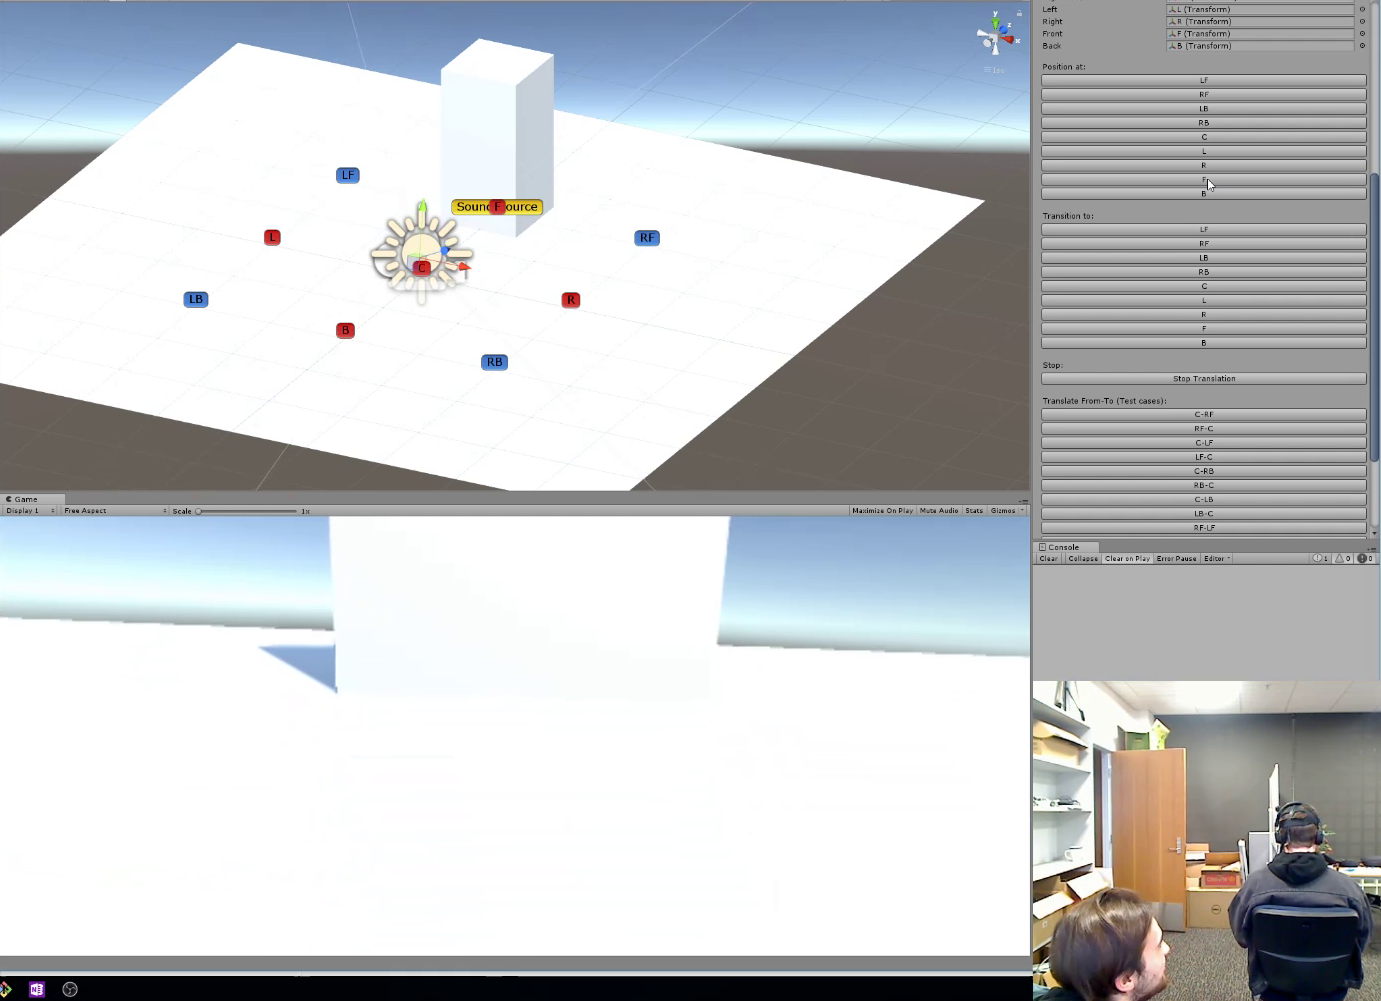
\includegraphics[width=0.7\linewidth]{figures/placeholders/pilot1_experiment_setup.png}
	\caption{Experiment setup}
	\label{fig:clipimage001}
\end{figure}

\begin{figure}
	\centering
	\subfloat[Predefined translation paths]{
		\label{fig:pilot1predefinedtutorialtranslations}
		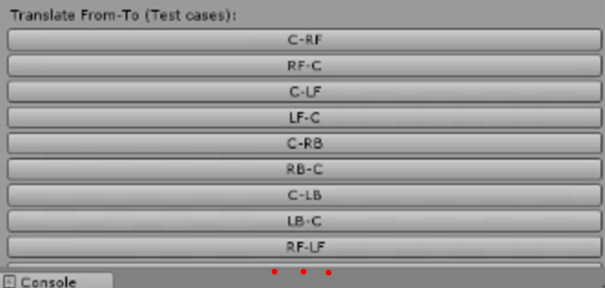
\includegraphics[width=0.3\linewidth]{figures/placeholders/pilot1_predefined_tutorial_translations}
	} %

	\subfloat[Arbitrary translations]{
		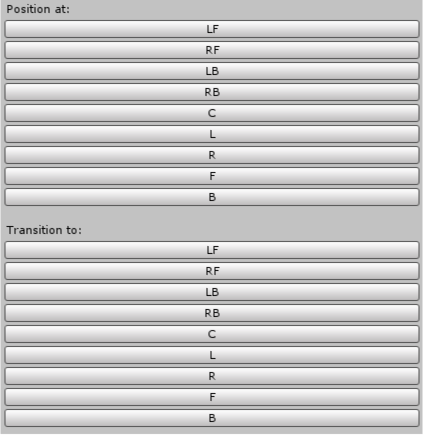
\includegraphics[width=0.3\linewidth]{figures/pilot1_control_panel}
		\label{fig:arbitrary_translation}
	}
	
	\caption{Control panels}
	\label{fig:pilot1controlpanel}
\end{figure}


\paragraph{Apparatus}
% Apparatus (i.e Unity, Resonance Audio, stereo headphones, Vive)
Experiment was implemented with the help of Unity3d  2018.1.5f1 and Resonance Audio SDK for Unity, version 1.2.1 with sound occlusion turned off. For the hardware, HTC Vive \gls{vr} headset, along with on-ear stereo headphones, and a Windows 10 PC.
Audacity 2.2.2 was used prior to the experiments to: mixdown stereo sounds to mono, make audio tracks seamless, and increase the volume.

% Study Factors and Conditions: what my factors are, conditions == independent variables' values
\paragraph{Study design}
The study followed the repeated measures design with 2 independent variables: translation speed and different types of auditory cues.

Three different translation speeds were tested: \textit{slow} - 20, \textit{medium }- 40, and \textit{fast }- 60 meters per second (m/s). Sound properties (i.e. pitch, playbackspeed) stayed constant throughout the different speeds.

Two different types of the auditory cues were tested: earcons and auditory icons. A full volume 100 Hz sine wave in mono was used for an earcon (Type: Wave (.wav), Samplerate: 44100.0 Hz, Bitdepth: 16bit, Source: https://freesound.org/people/klangfabrik/sounds/28638/, Fig. \ref{fig:pilot1sinewaveedit}). As an auditory icon a mono sound mimicking moving concrete block with sound amplitude extrema reaching full volume was used (Type: Wave (.wav), Samplerate: 48000.0 Hz, Bitdepth: 16 bit, Source: https://freesound.org/people/FreqMan/sounds/25846/, Fig. \ref{fig:pilot1concreteonconcretesoundedit}).
The type of sound played first was rotated for the participants, so that 4 of them heard the auditory icon first, and the other 4 - the earcon.

\begin{figure}
	\centering
	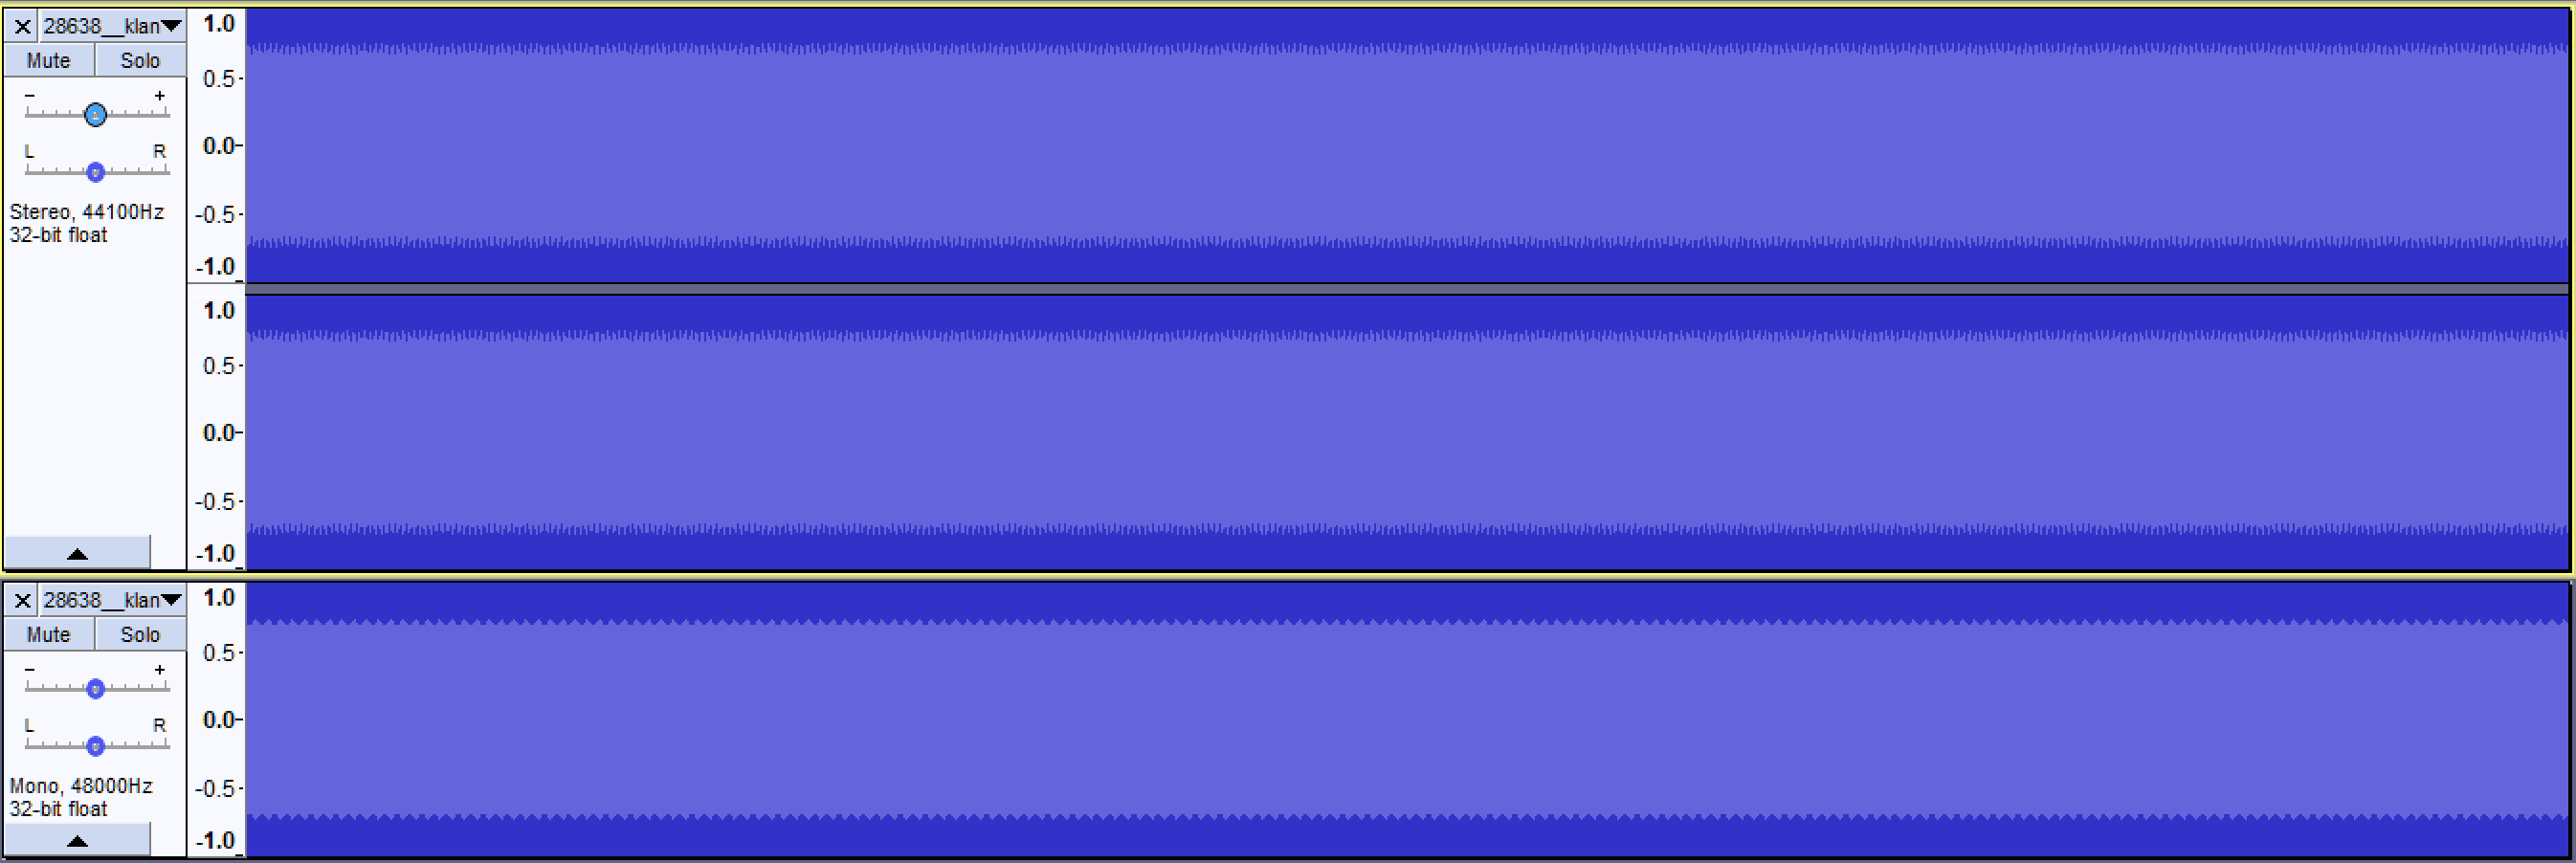
\includegraphics[width=0.7\linewidth]{figures/pilot1_sinewave_edit}
	\caption{Sine wave earcon before (top) and after (bottom) mixdown: stereo to mono}
	\label{fig:pilot1sinewaveedit}
\end{figure}

\begin{figure}
	\centering
	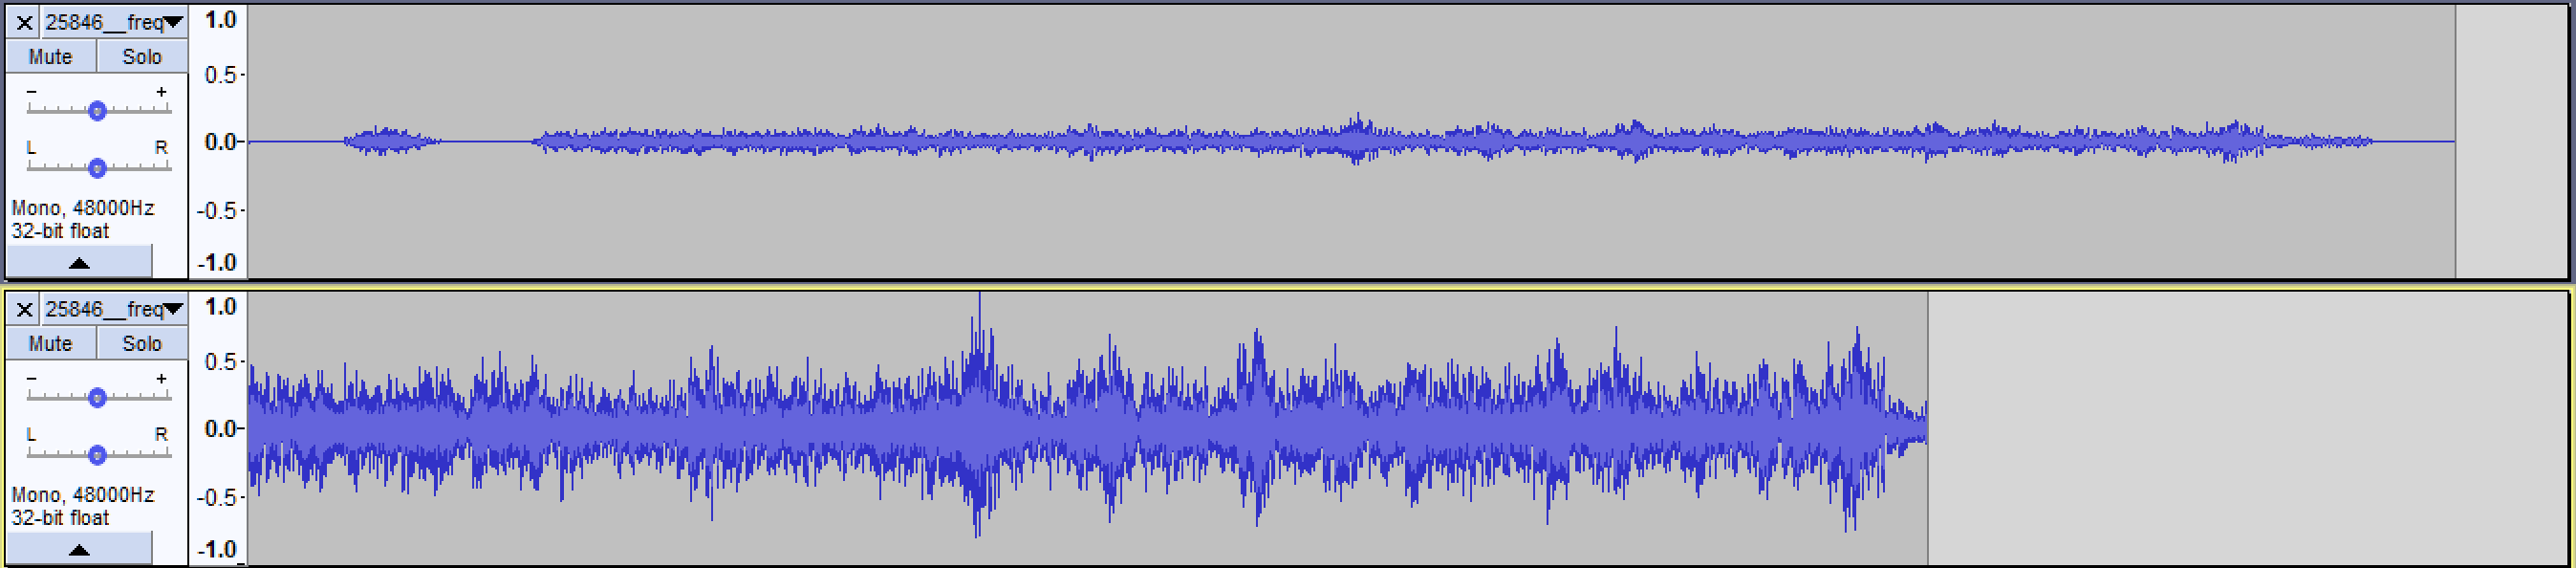
\includegraphics[width=0.7\linewidth]{figures/pilot1_concrete_on_concrete_sound_edit}
	\caption{Concrete sliding on concrete auditory icon before (top) and after (bottom) amplification, and crop}
	\label{fig:pilot1concreteonconcretesoundedit}
\end{figure}

Translations were pseudo-randomized across participants, their selection was made with some degree of bias towards longer translation paths, so that users have more time to analyze the sound and guess (i.e. the path from RB to LB would be longer, than just RB to B). Different translation paths can be seen in Fig. \ref{fig:pilot1translationpaths}.

Distances between the fixed translation end-points remained the same throughout the experiment: 20 Unity3d units (meters) between C-F, C-L, C-R, C-B, L-LB, and so on.

\paragraph{Results}
\textit{Preferred sound} 6 out of 8 participants preferred the concrete sound to the sine wave, 1 was indifferent as long as the speed was slow, and 1 preferred the sine wave.

\textit{Preferred speed} The speed preference can be seen in the Table \ref{table:pilot1_results}.

\begin{figure}
	\centering
	
	\subfloat[Top-down view of the scene]{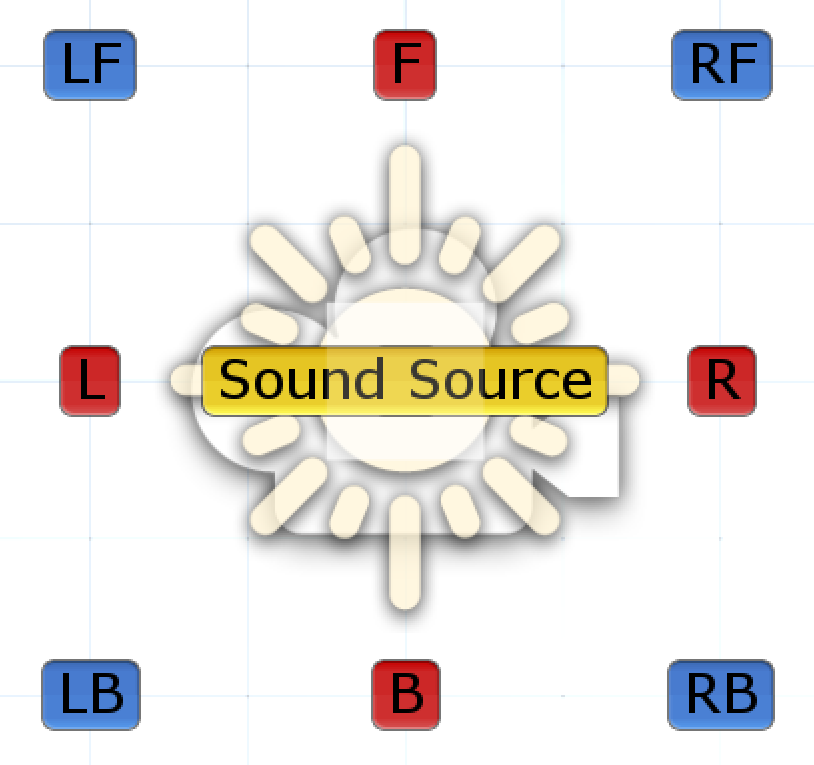
\includegraphics[scale=.4]{figures/pilot1_top_down_scene_view.png}}%
	\subfloat[Major translation paths]{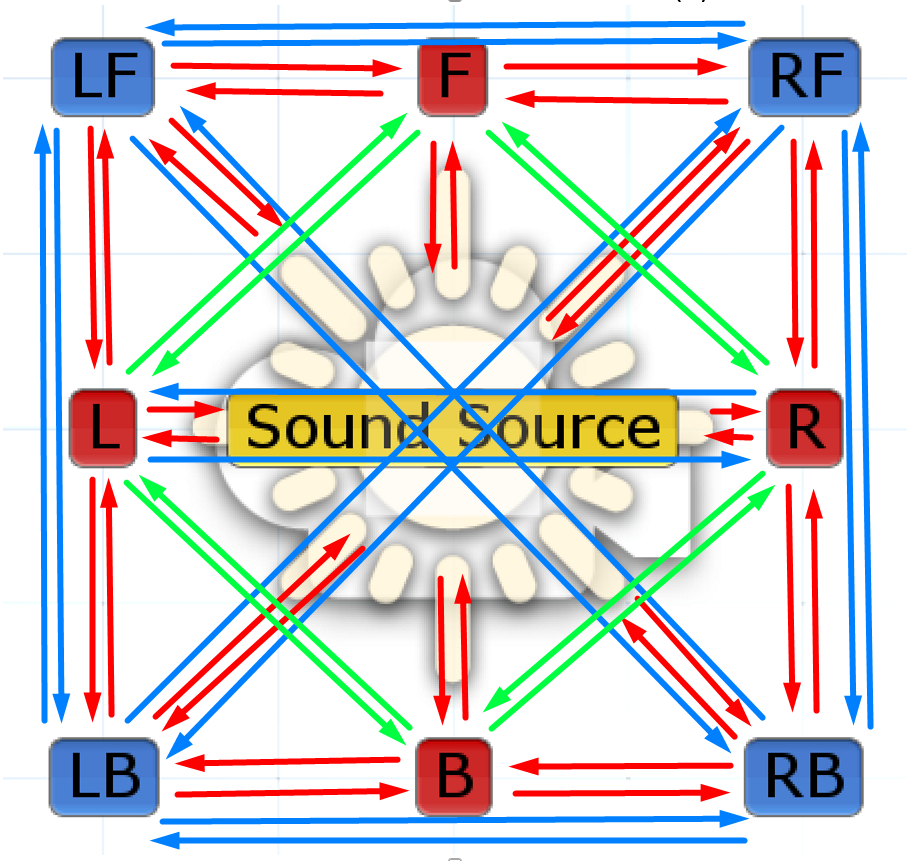
\includegraphics[scale=.4]{figures/pilot1_top_down_scene_view&major_tranlsation_paths.png}}%
	\subfloat[All translation paths]{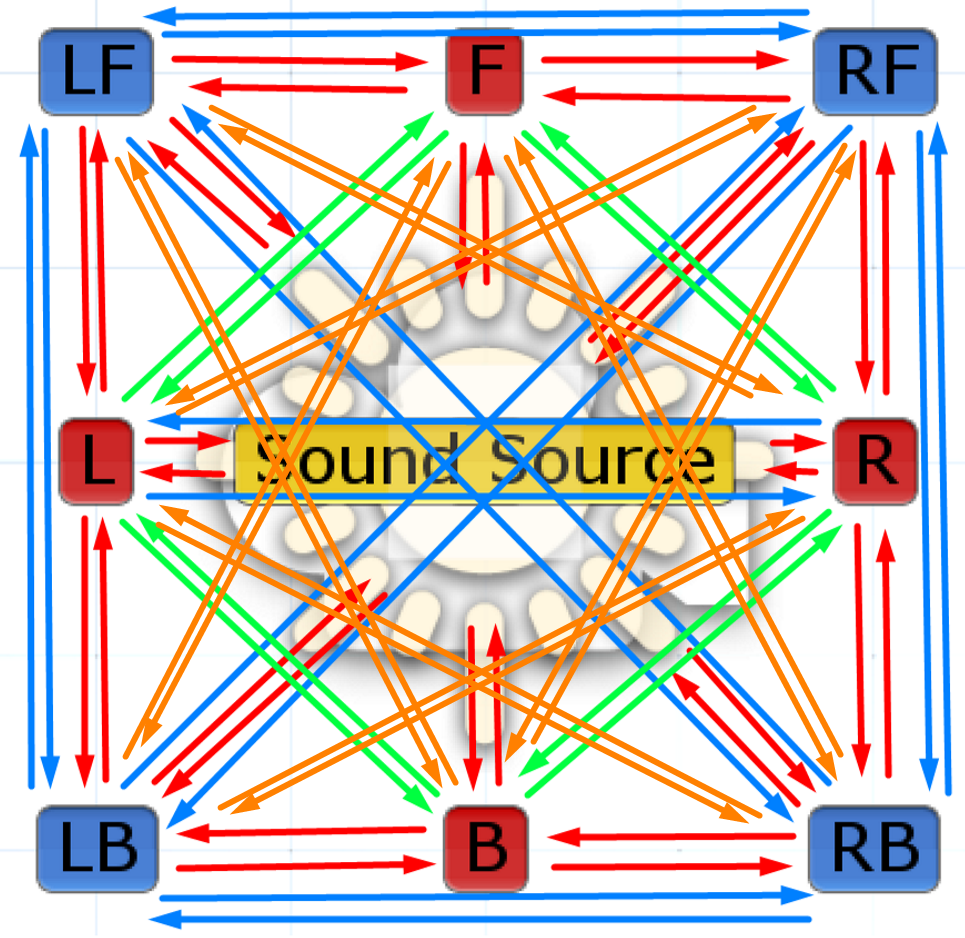
\includegraphics[scale=.4]{figures/pilot1_top_down_scene_view&all_possible_translation_paths.png}}
	
	\caption{Possible translation end-points and paths}
	\label{fig:pilot1translationpaths}
\end{figure}


\begin{table}[h]
	\label{table:pilot1_results}
	\caption{Experiment data}
	
	\begin{tabular}{|l|l|l|l|}
		\hline
		\textbf{Participant} & \textbf{First sound played} & \textbf{Preferred sound} & \textbf{Preferred speed}                        \\ \hline
		1                    & Concrete                    & Concrete                 & Medium                                          \\ \hline
		2                    & Concrete                    & Concrete                 & Slowest, then medium                            \\ \hline
		3                    & Sine wave                   & Concrete                 & Medium                                          \\ \hline
		4                    & Sine wave                   & Concrete                 & First two -fine (fastest one - a bit too fast)  \\ \hline
		5                    & Concrete                    & Either                   & Slowest                                         \\ \hline
		6                    & Sine wave                   & Sine wave                & Fast (speed didn't affect it too much)          \\ \hline
		7                    & Concrete                    & Concrete                 & Between slow and medium                         \\ \hline
		8                    & Sine wave                   & Concrete                 & First two - fine (fastest one - a bit too fast) \\ \hline
	\end{tabular}
\end{table}

\paragraph{Discussion}
If we visualize the participants' preferences, and take the smallest common area, where they overlap, analysis shows that participants preferred the speed somewhere close to 40 m/s, but between 20 and 40 (Fig. \ref{fig:pilot1resultsanalysis})

The preferred (concrete on concrete) sound, which was described by one participant as "dry and dull", has a distinct timbre, which is made of different harmonics and halftones. The sine wave, on the other hand, has only 1 fundamental frequency, which might make memorizing and spatial differentiation harder. Additionally, this frequency would most likely get cut of by the audio SDK, if occlusion effect was to be used.

\begin{figure}	
	\centering
	
	\subfloat["Medium"]{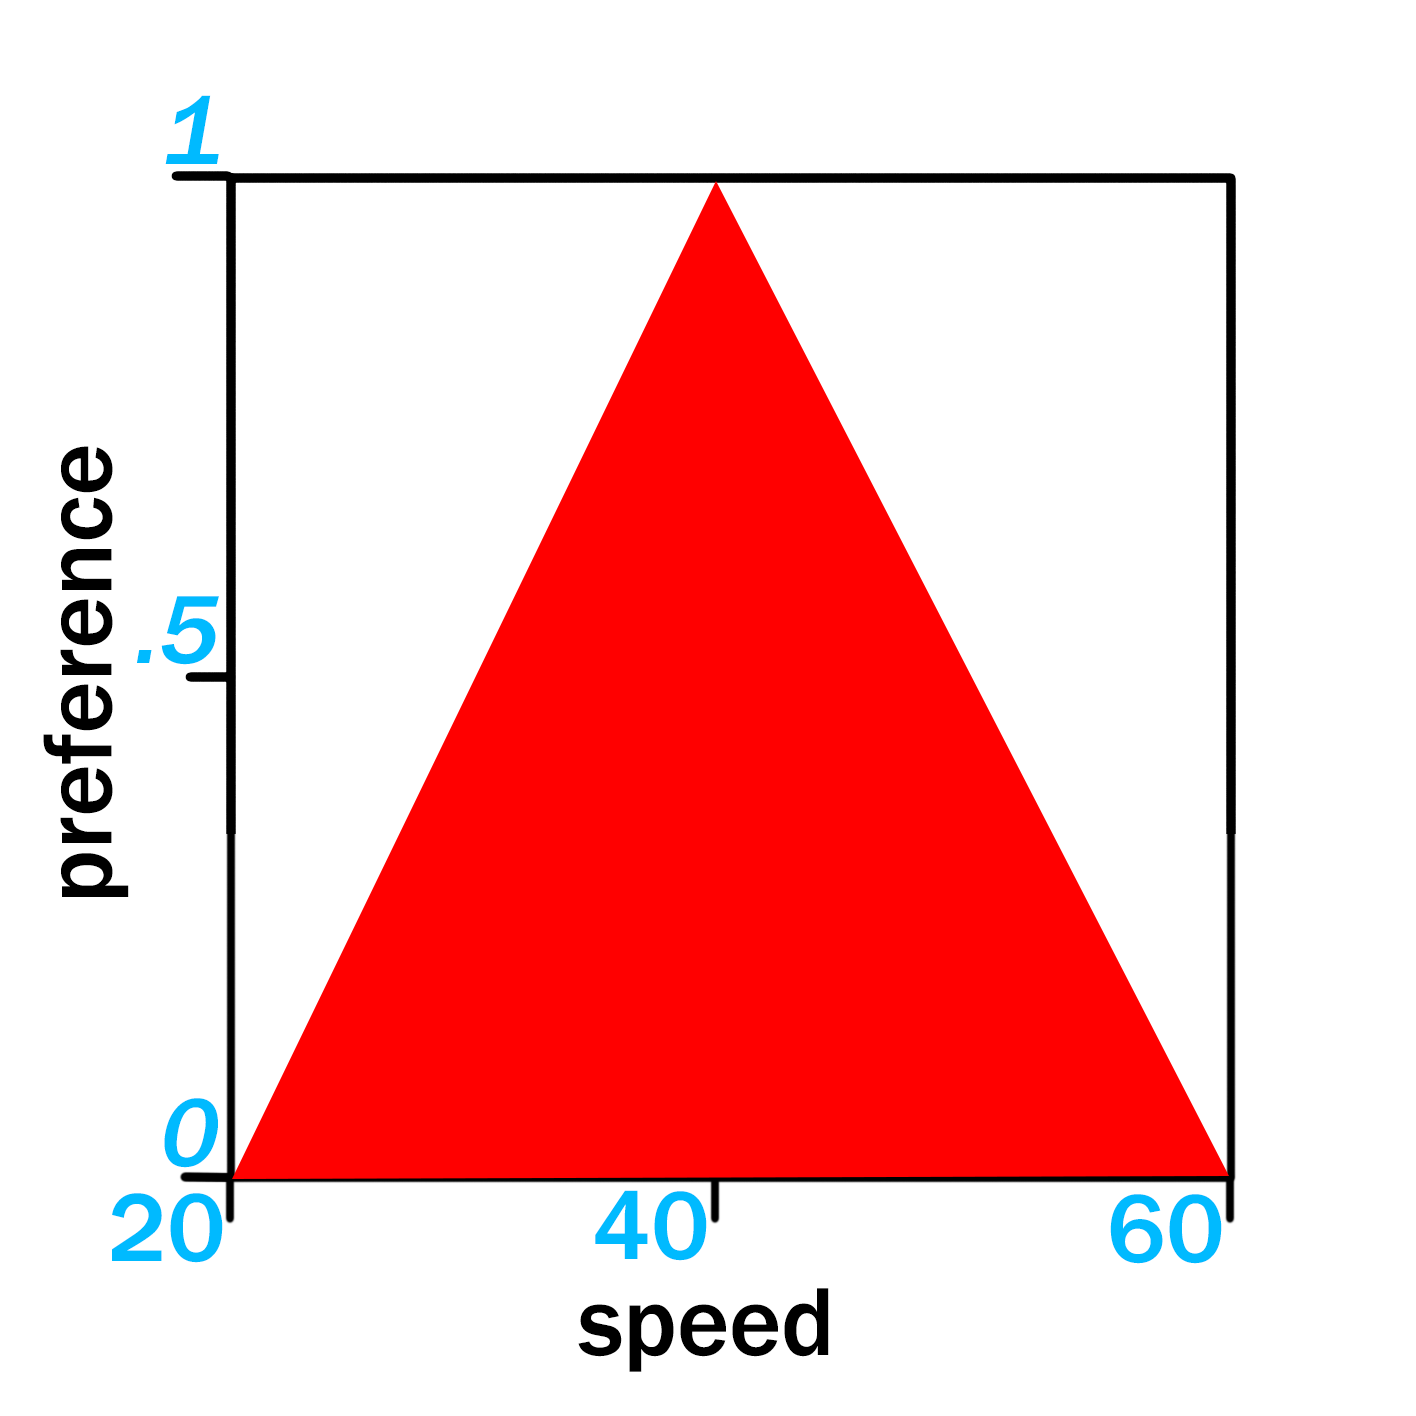
\includegraphics[scale=.075]{figures/pilot1/results/speed_fuzzy_preference_medium.png}}%
	\subfloat["Slowest, then medium"]{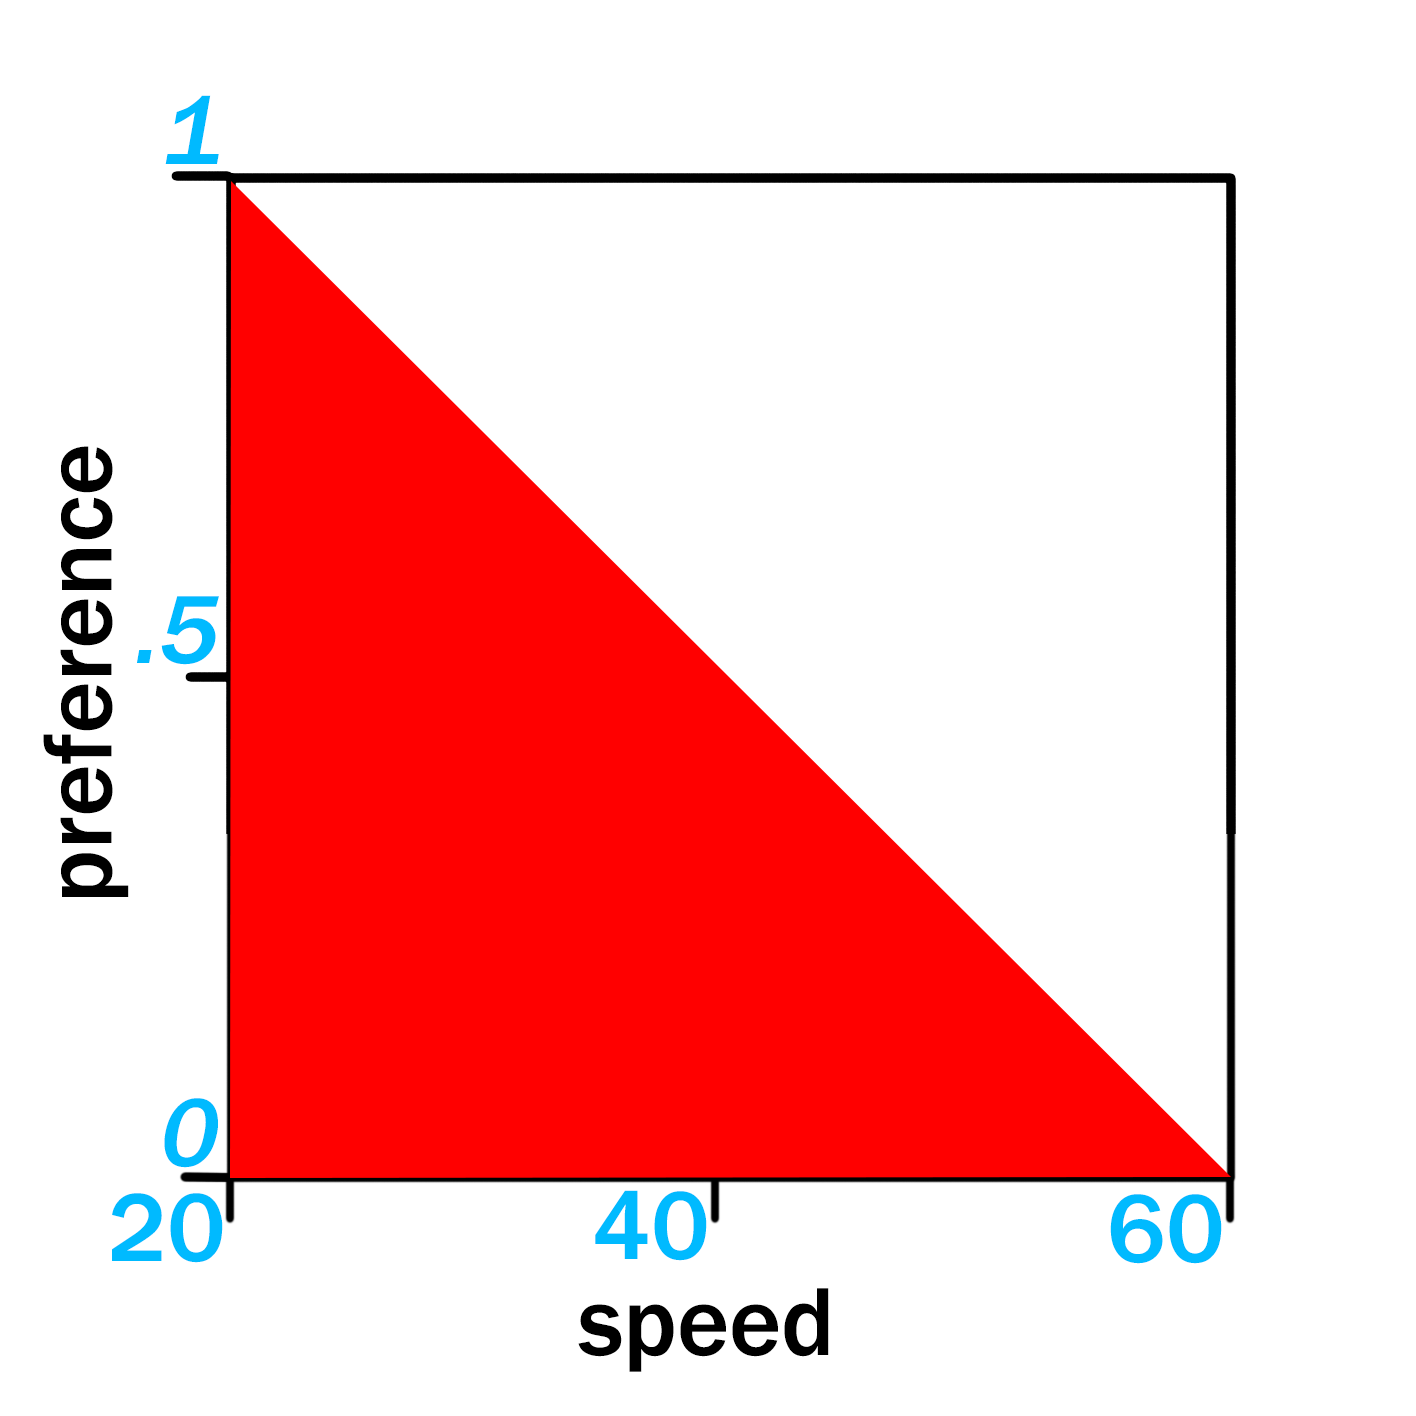
\includegraphics[scale=.075]{figures/pilot1/results/speed_fuzzy_preference_slowest_then_medium.png}}%
	\subfloat["First two - fine..."]{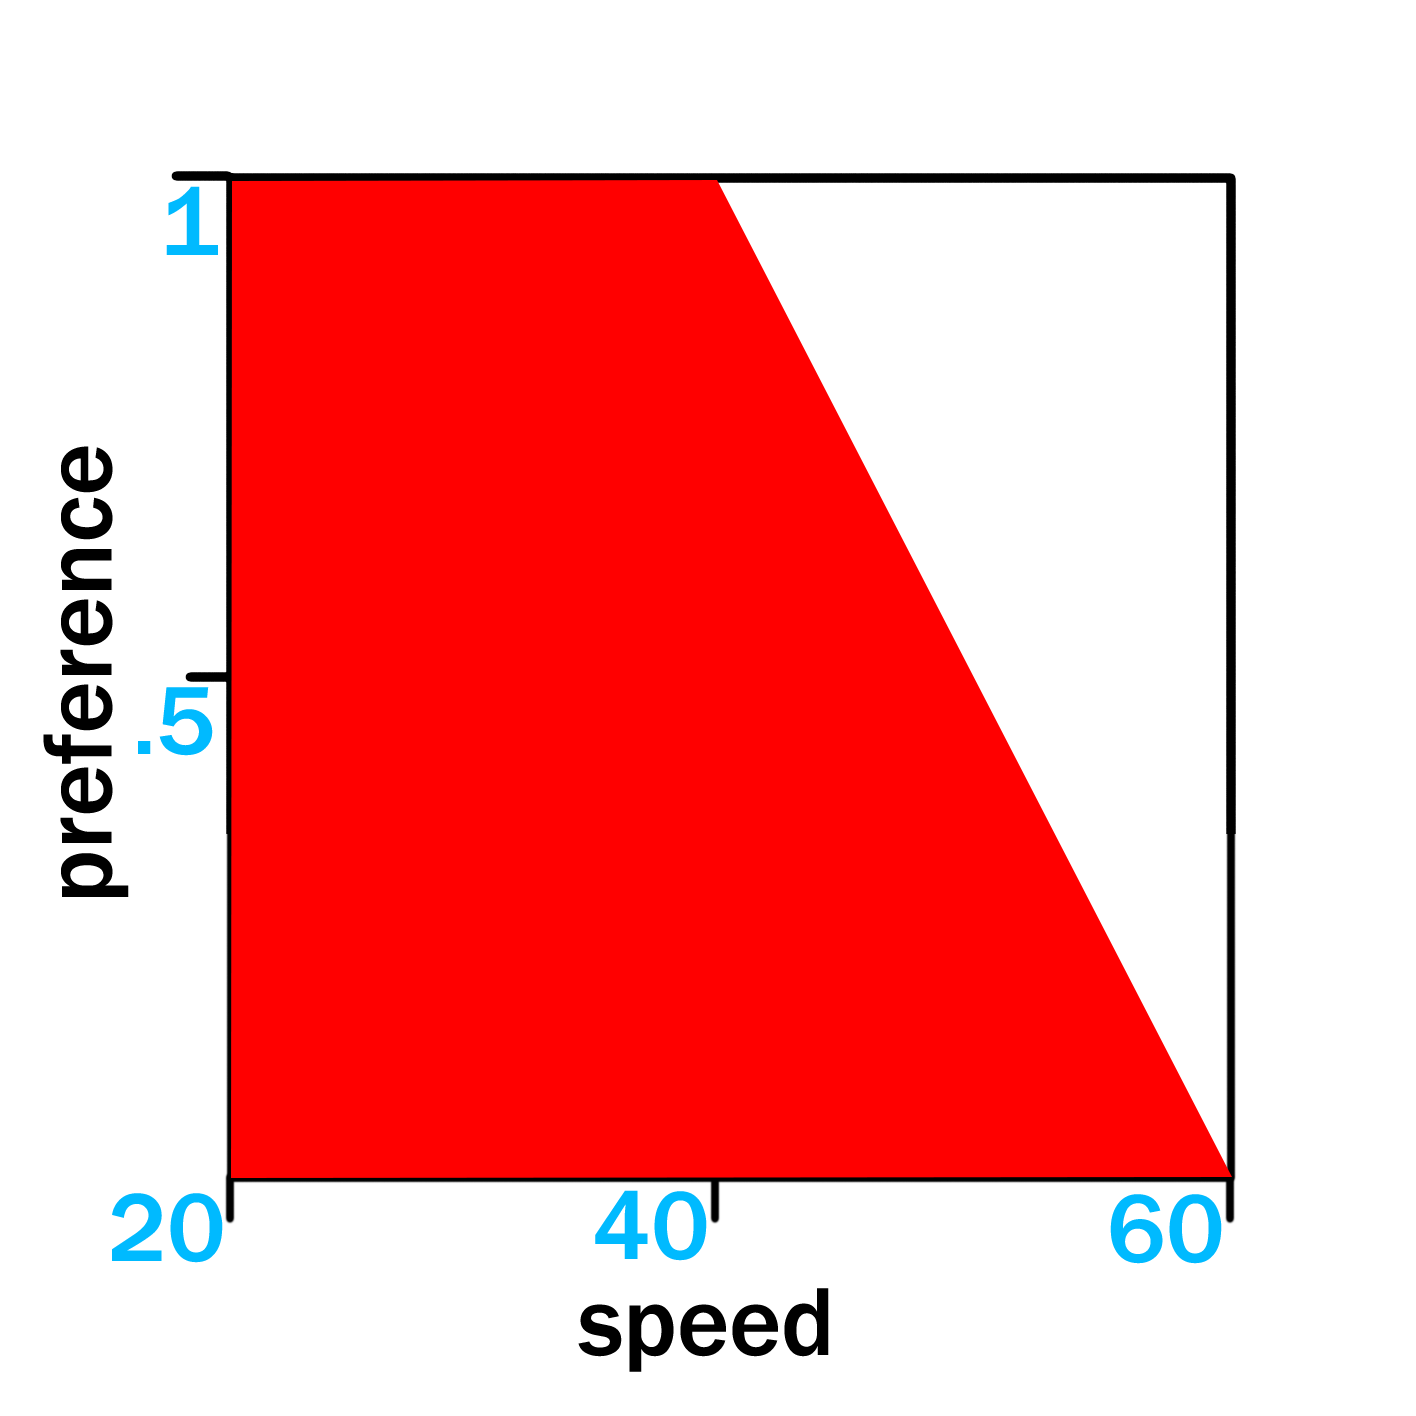
\includegraphics[scale=.075]{figures/pilot1/results/speed_fuzzy_preference_first_two_fine.png}}%
	\subfloat["Slowest"]{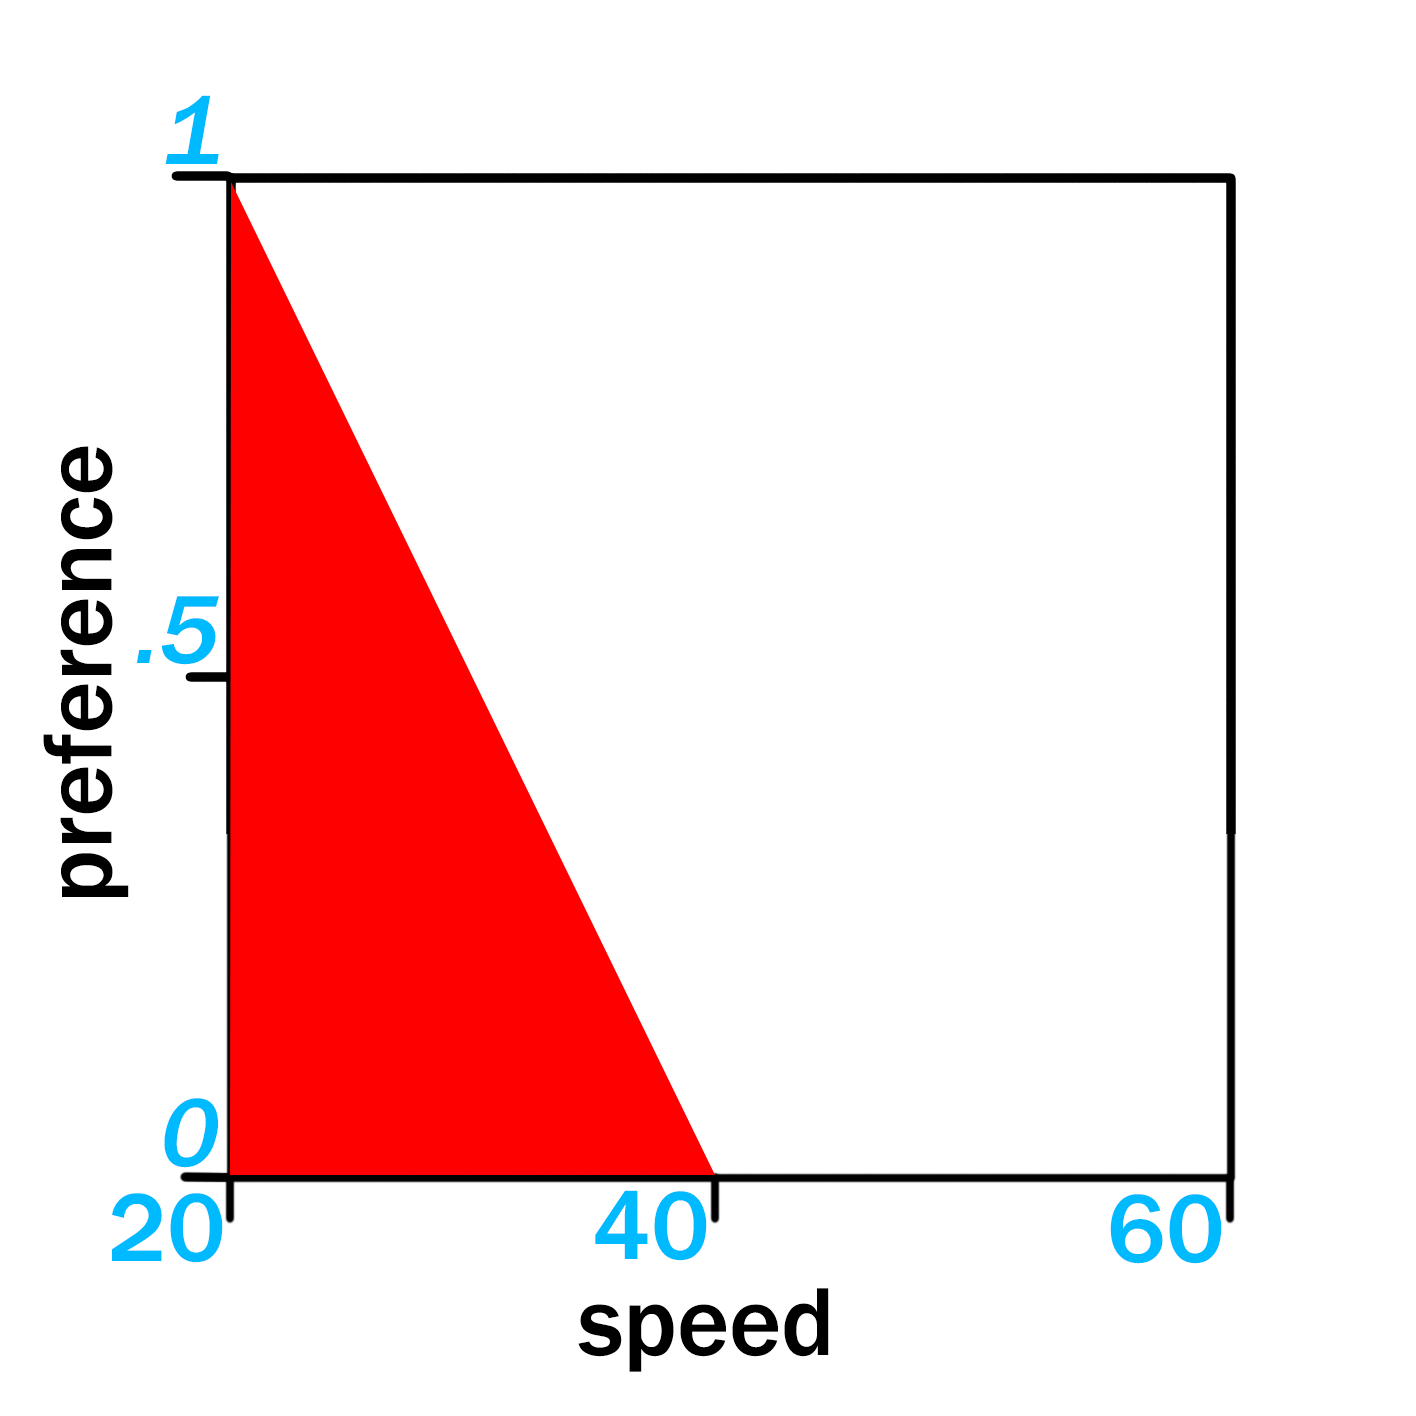
\includegraphics[scale=.075]{figures/pilot1/results/speed_fuzzy_preference_slowest.png}}
	
	\par\medskip
	\subfloat["Fast..."]{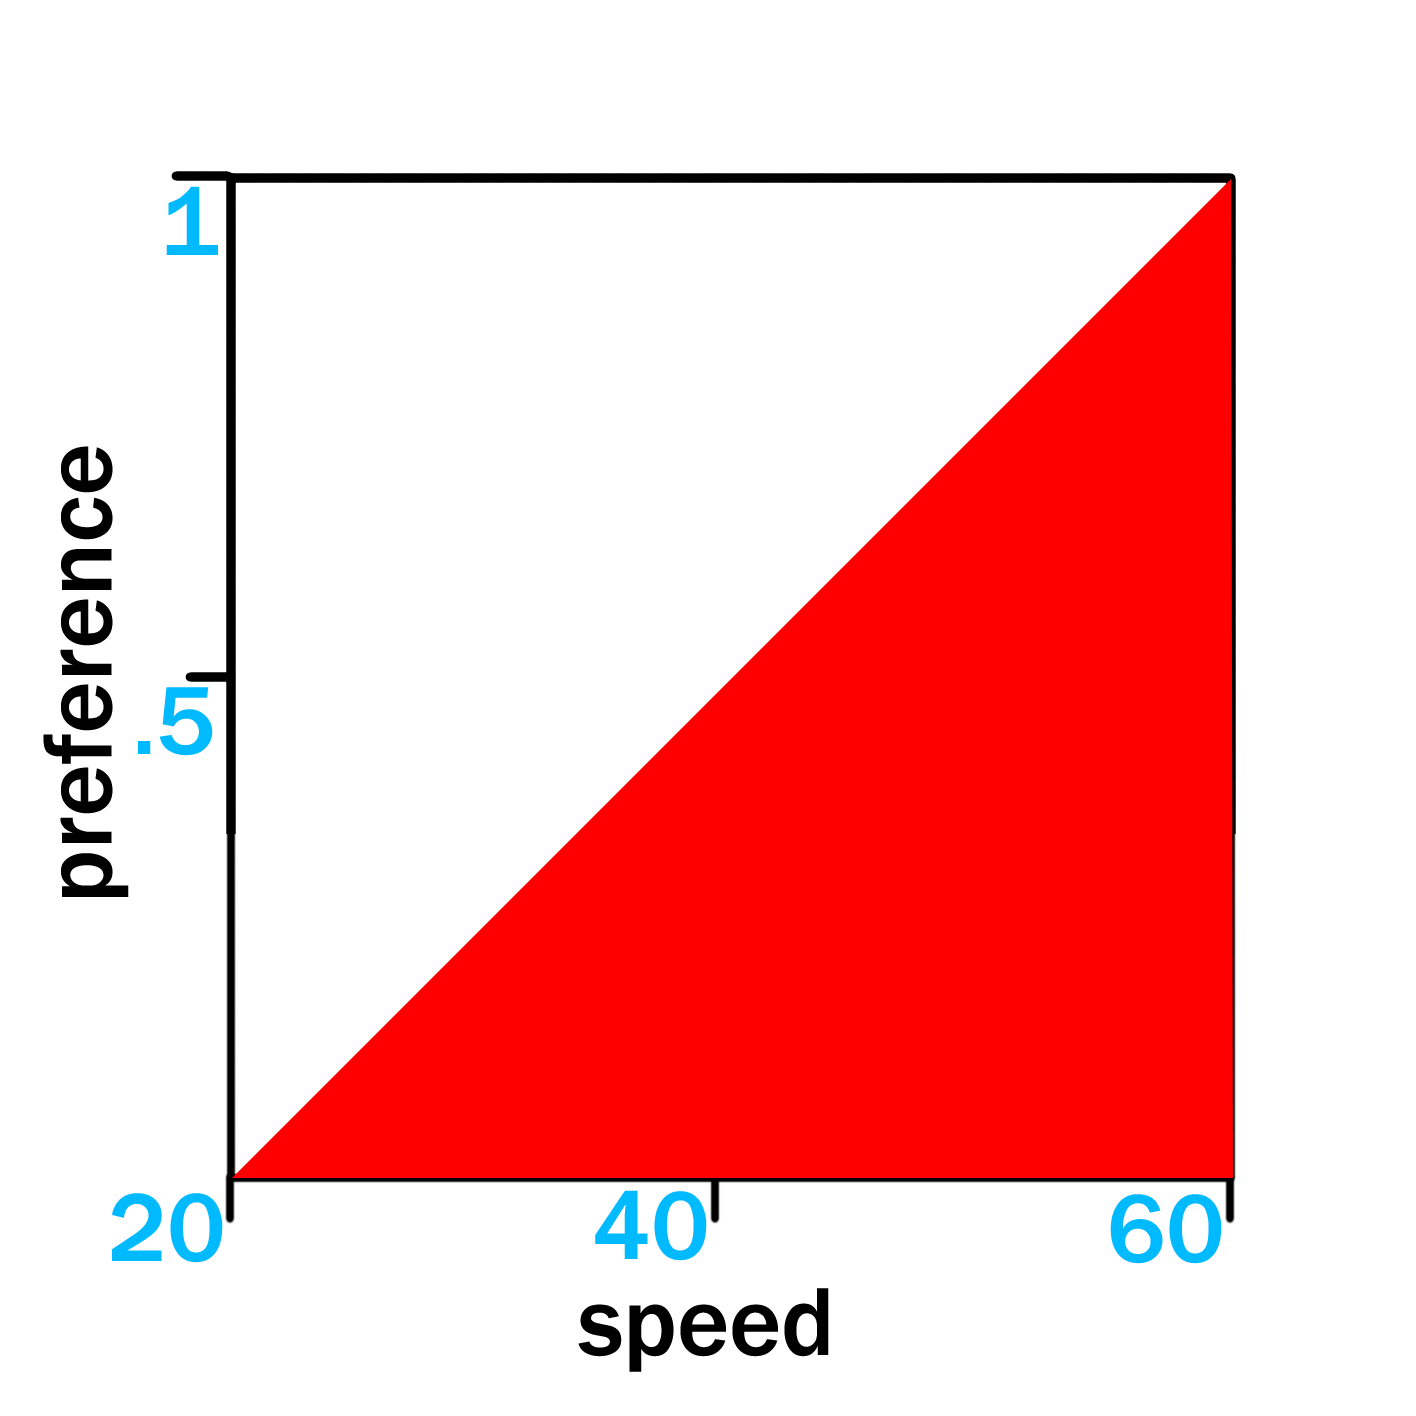
\includegraphics[scale=.075]{figures/pilot1/results/speed_fuzzy_preference_fast.png}}%
	\subfloat["Between slow and medium"]{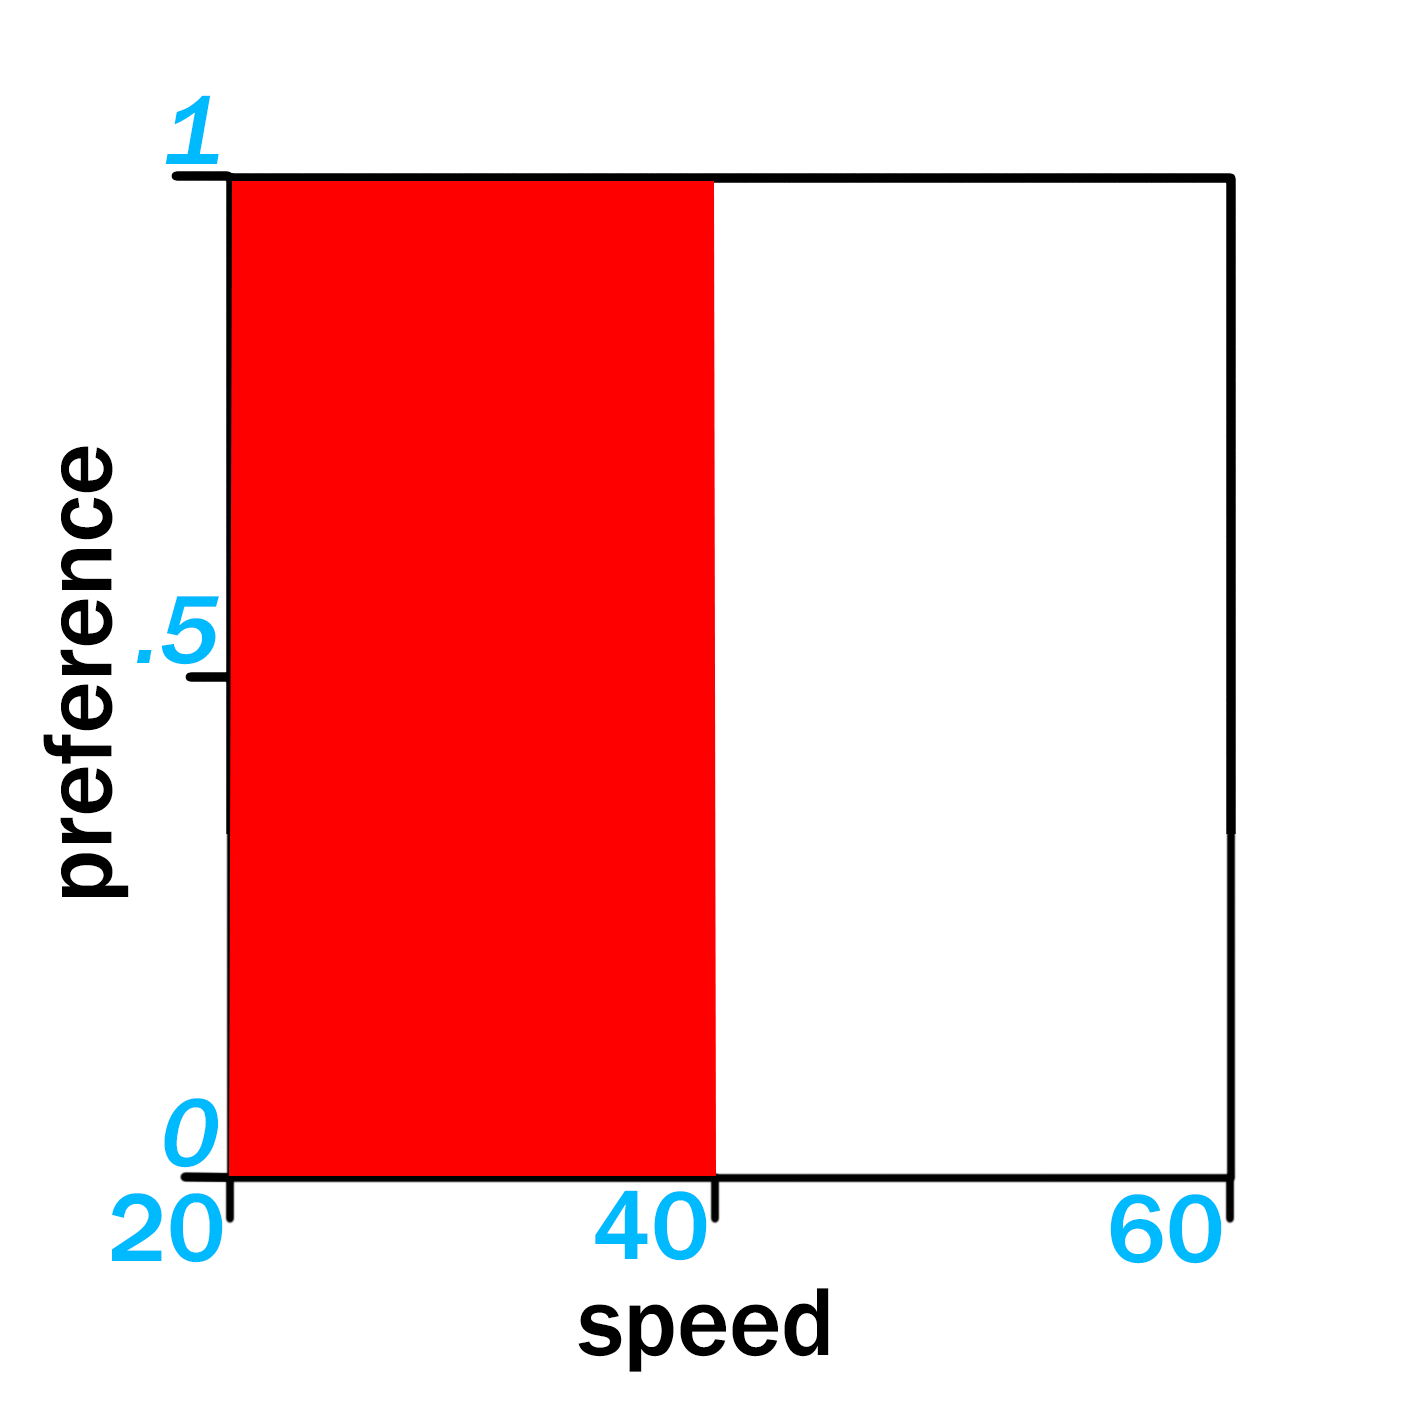
\includegraphics[scale=.075]{figures/pilot1/results/speed_fuzzy_preference_between_medium_and_slow.png}}%
	\subfloat[Answers combined with 12\% opacity each]{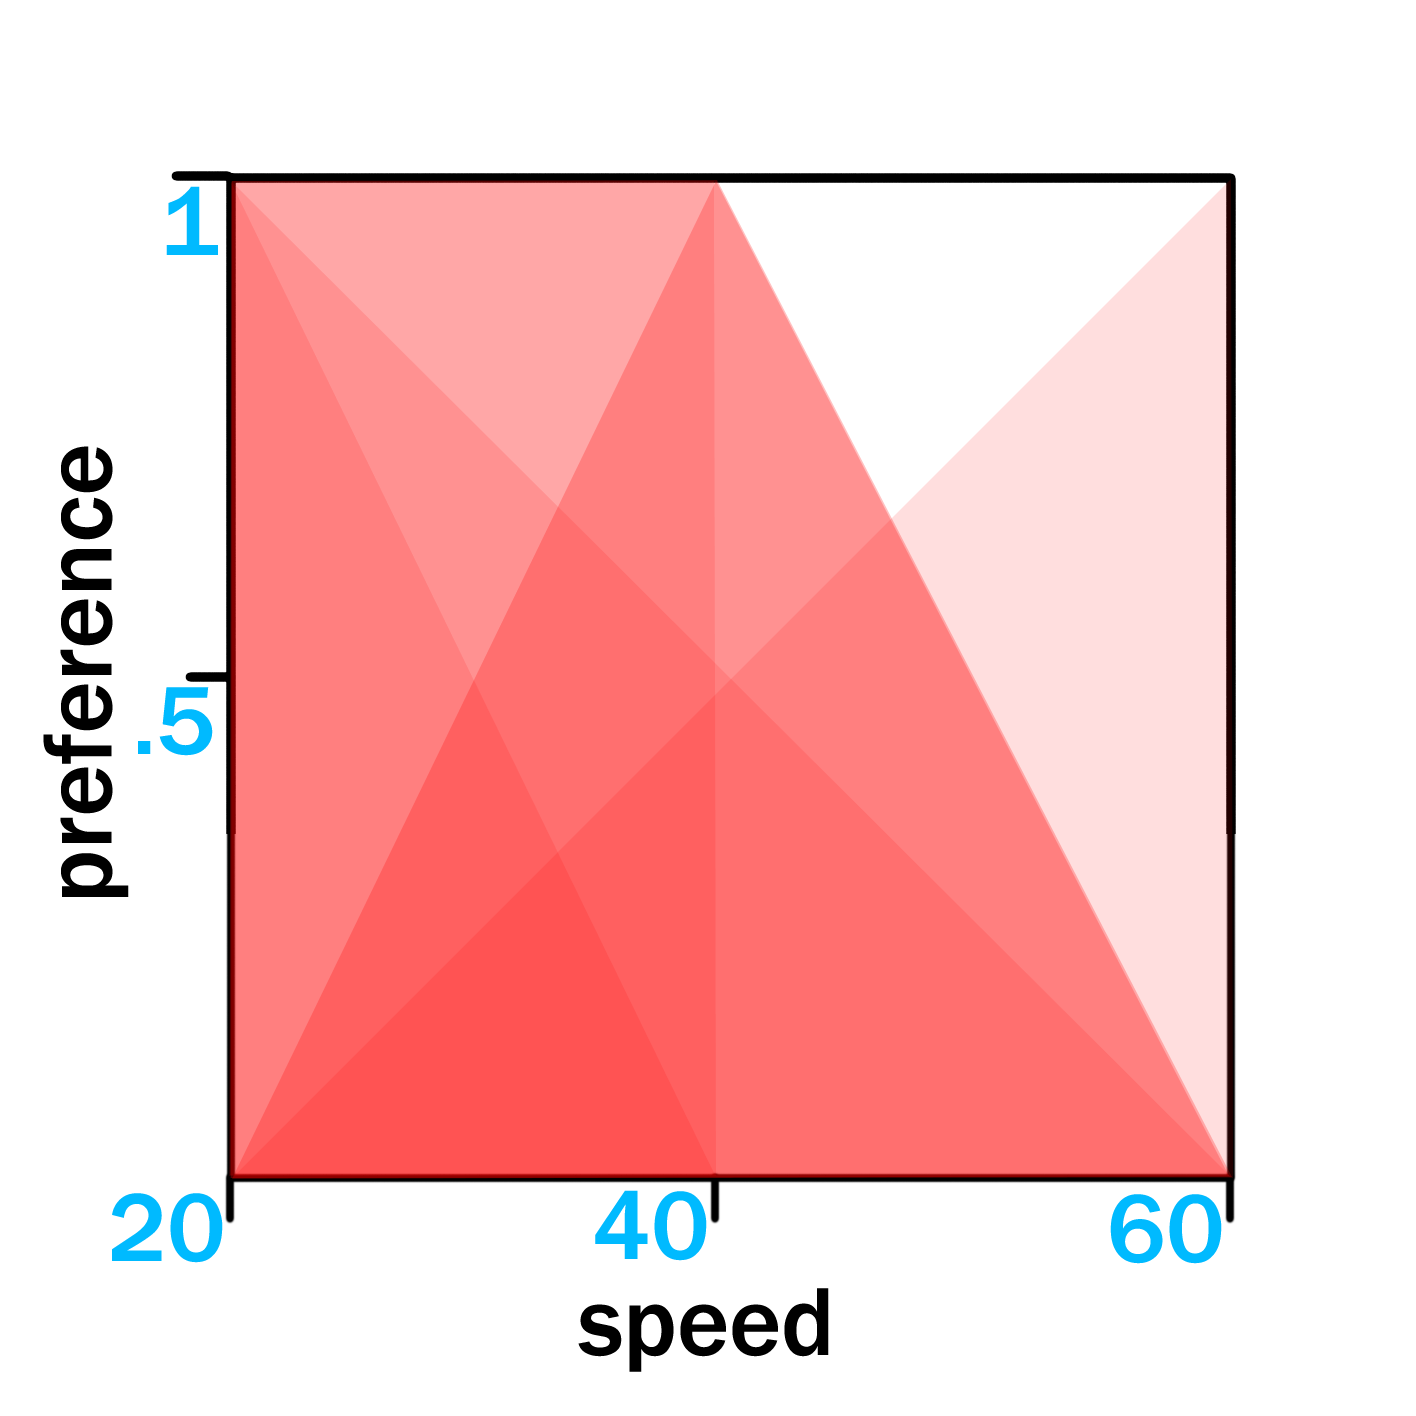
\includegraphics[scale=.075]{figures/pilot1/results/speed_fuzzy_preference_result_no_highlight.png}}	
	
	\par\medskip
	\subfloat[Preferred speed according to analysis]{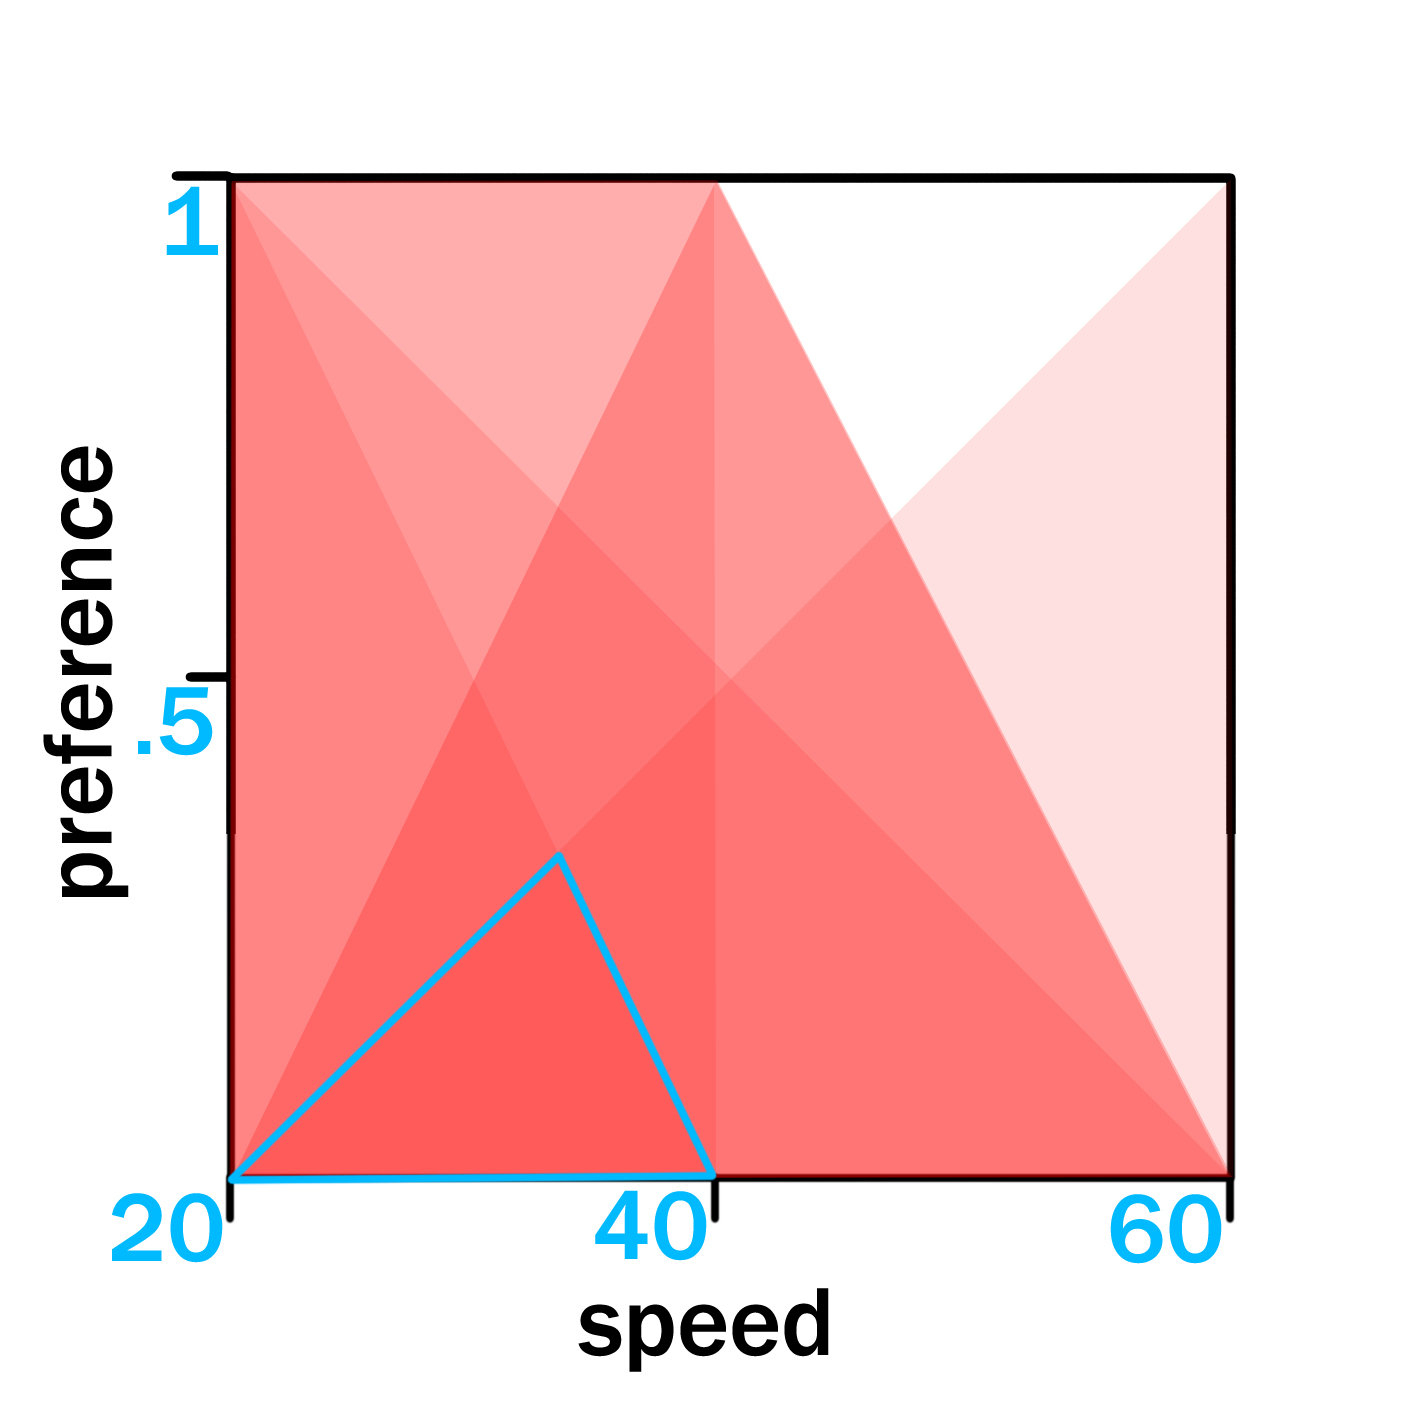
\includegraphics[scale=.15]{figures/pilot1/results/speed_fuzzy_preference_result.png}}
	
	\caption{Visual analysis of results, pilot 1}
	\label{fig:pilot1resultsanalysis}
\end{figure}

\subparagraph{Limitations} 
\textit{Auditory variation} Only 2 different types of auditory cues were used in this study to indicate the translation of the building. Different sounds might need to be tested to take advantage of different sound properties on the ability to interpret the spatial sound. 

\textit{Front-to-back confusion} One of the major observation was the inability of participants to differentiate between translations happening in the back and in the front. For example, the translation from RF to LF was mistakenly indicated as RB to LB. The reason for this is the use of stereo headphones, which do not provide intuitive spatial cues for sounds happening in front and in the back of the user.
%The confusion between front to back has to been pointed out to might have something to do with the sound reproduction in stereo headphones

\textit{Visualization} As it was a preparatory study, the participants were simply asked to close their eyes when guessing the path of the building. Besides the obvious drawback of such approach, participants reported that it is possible to predict the path by relying on the change in brightness, which is perceivable even with the eyes closed, when the building is passing by.

\textit{False negatives} Some users, who gave answers that were close to correct (i.e. the building was reported to move from R to LB, when in reality it moved from RB to LB), indicated that they were not aware that the building can move along such a path.









\subsection{Spatial Judgment}
\label{study_two}
%Goal
The goal of this pilot study was to see how much information about the buildings moving in the environment could be conveyed through stereo headphones with the current setup. Additional motivation was to pilot the way for participants to point out the changes to the environment, which would be needed in the final study to infer the \gls{wa} index. 

\paragraph{Participants}
Thirteen participants (9 men and 4 women; mean 29.4, std. 10.7) were selected from the employees and students at the University of Otago, New Zealand. 10 had good amount of prior experience with \gls{vr}, 8 reported good hearing, and 6 were regular online gamers. More detailed data about the participants can be found in Appendix \ref{app:pilot2questionnaire_data}. Most of the participants from the first pilot study took part in the second.

\paragraph{Procedure \& Task}
Participants were welcomed and asked to fill out the questionnaire (Appendix \ref{app:pilot2questionnaire_data}) prior to the experiment. Next, the goals of the study, the project, and the tutorial were explained along with participant's individual task. Next, participants were put into the \gls{vr} environment to begin the tutorial.

This \gls{vr} environment was constructed specifically for this experiment. This environment had 2 modes: tutorial and experiment (Fig. \ref{fig:pilot2experiement_environment}). In both of them, the participant would appear at the middle of the scene. There was a real-sized building and a cylindrical wall around the participant with the center at their position. The building was approximated with a cuboid extended along the vertical axis. Like in the previous pilot, this building would emit sound, when it translated through the scene.
% TODO: add tutorial, back view sreenshot
\begin{figure}
	\centering
	\subfloat[Tutorial mode, the building (front view)]{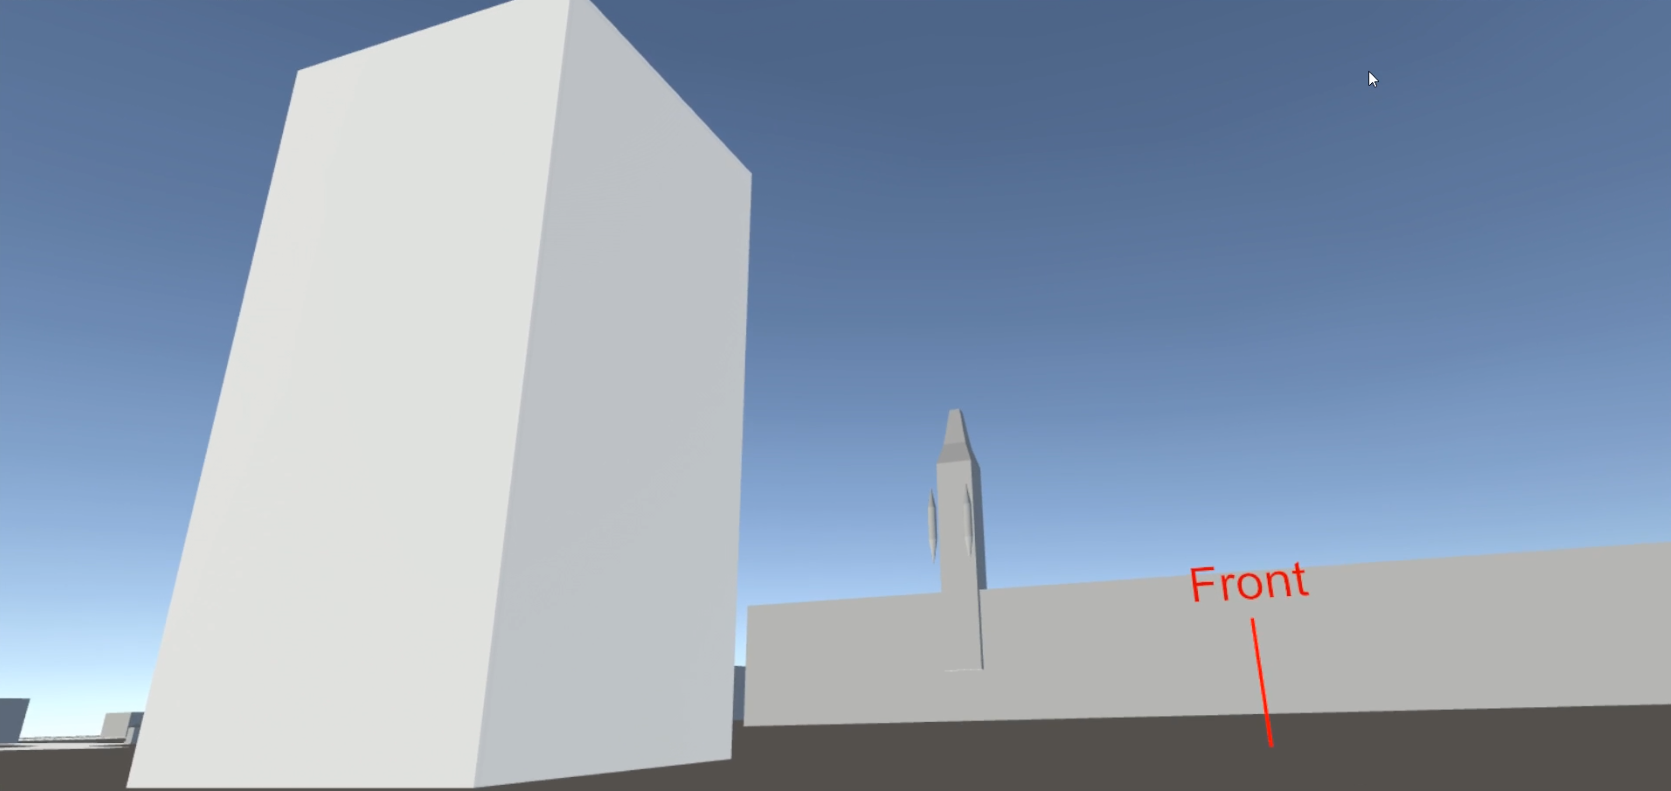
\includegraphics[width=0.7\linewidth]{figures/pilot2_environment_tutorial}}
	\par
	\subfloat[Experiment mode, the cylinder wall (front view)]{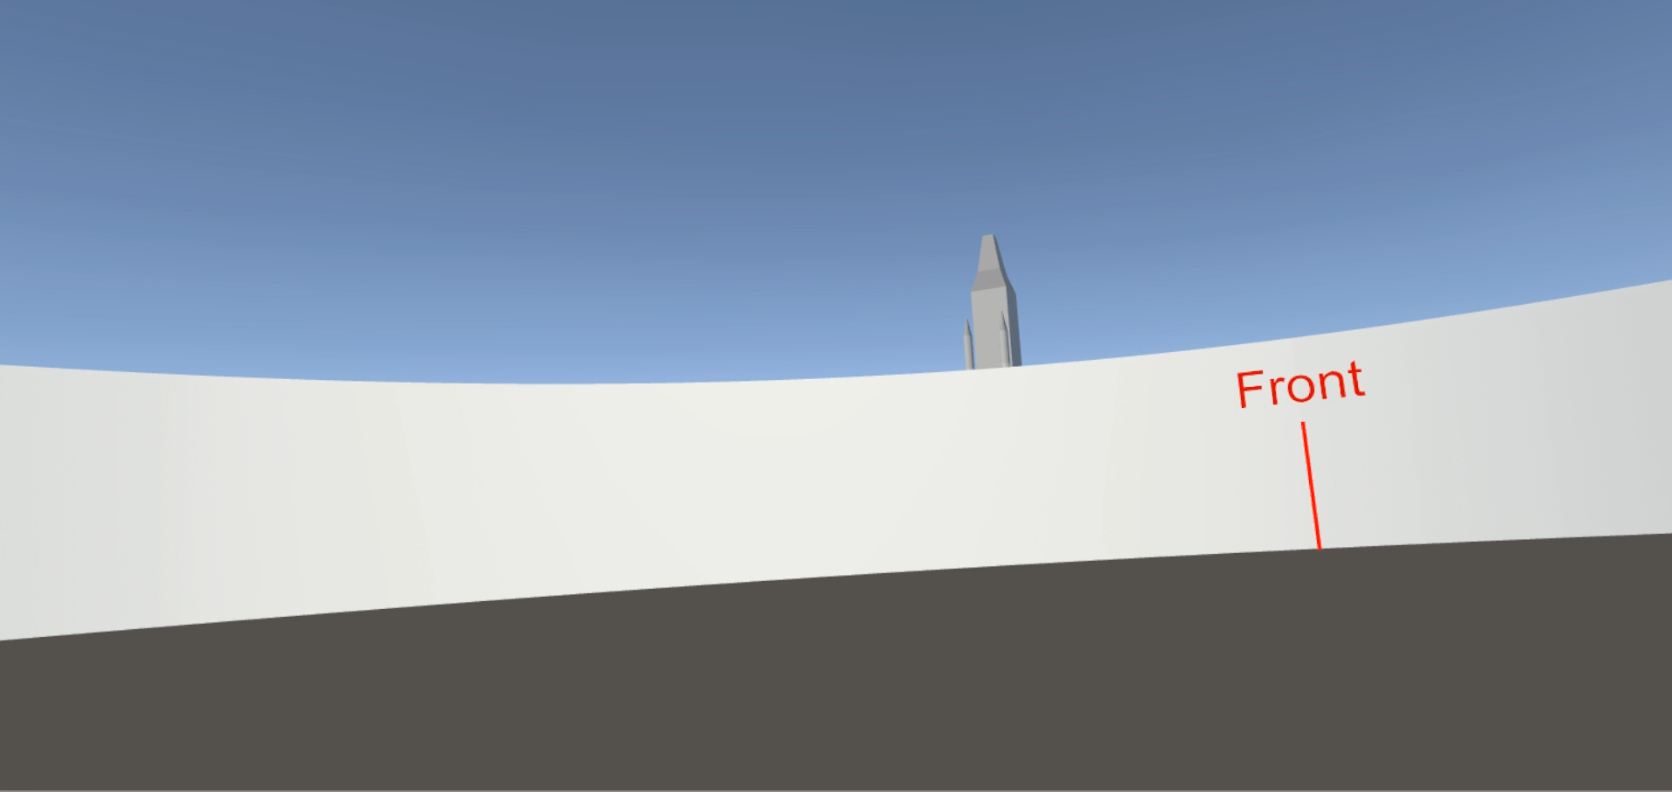
\includegraphics[width=0.7\linewidth]{figures/pilot2_tutorial_experiment_front}}
	\par
	\subfloat[Experiment mode, the cylinder wall ()back view)]{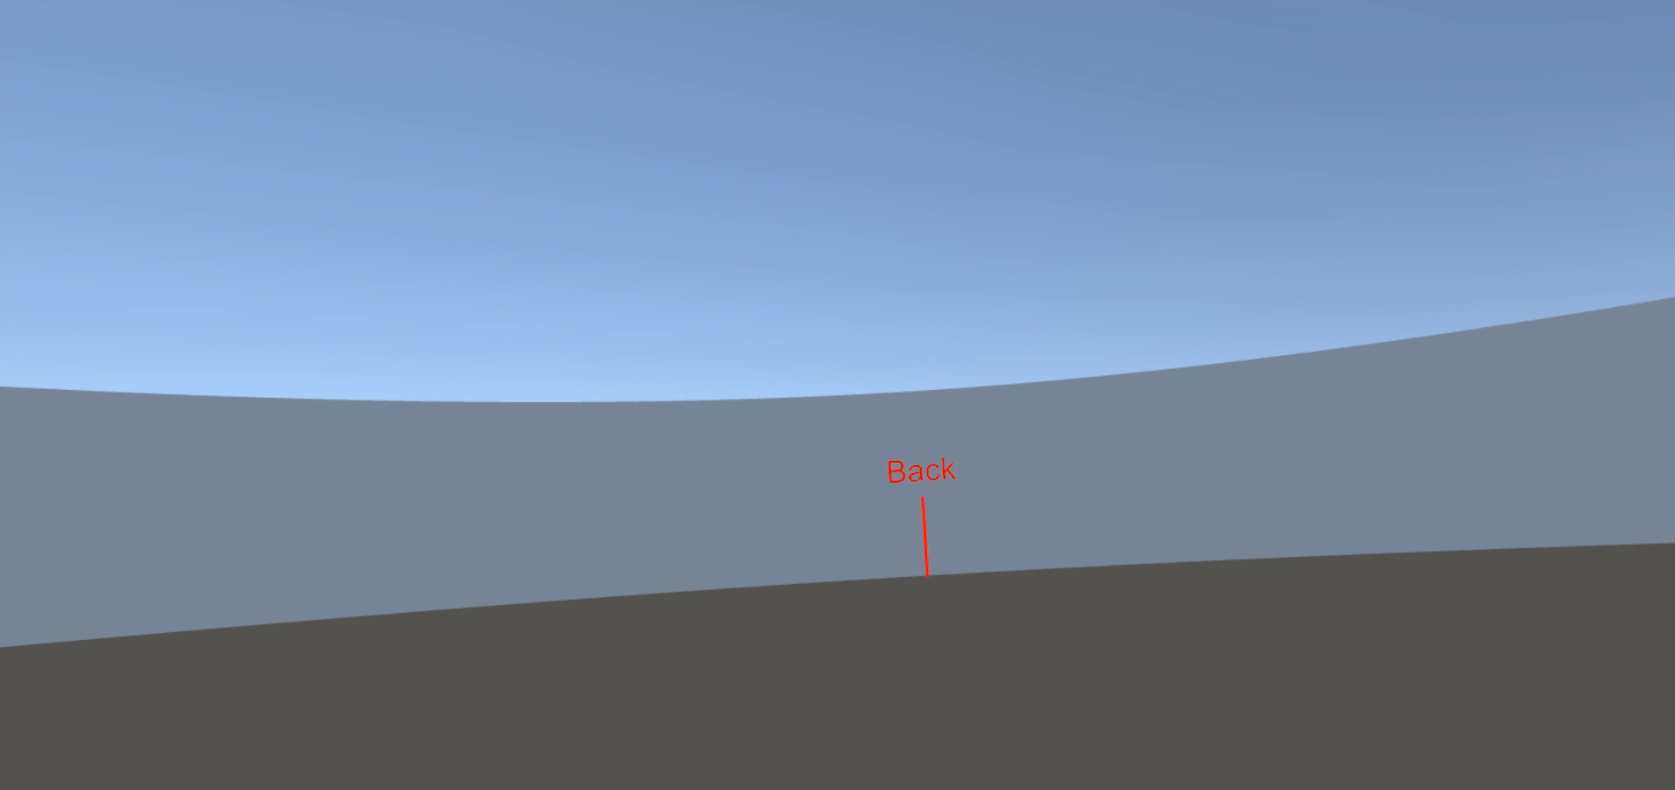
\includegraphics[width=0.7\linewidth]{figures/pilot2_tutorial_experiment_back}}
	\caption{Experiment environment}
	\label{fig:pilot2experiement_environment}
\end{figure}

% TODO: the participant, a participant, participant, participants?
The goal of the tutorial mode was to allow the participant to understand the correlation between the visually perceived movements of the building and the sound emitted. The affordances of the environment were explained prior to the tutorial.

In the tutorial mode, the building was visible, and the wall - invisible.
40 translations were pre-scripted for the actual experiment, 20 of which were demonstrated. The control panel for this experiment can be viewed in Fig. \ref{fig:pilot2tutorialcontrolpanelhighlighted}, the buttons that are highlighted in blue were used to initiate tutorial translations. These translations were initiated in the same order for all the participants, they are additionally visualized in Fig. \ref{fig:pilot2endpointstutorialtranlstaions}.

Participants were briefed to face the "Front" direction, when the experimenter voiced the path that the building was going to travel, or (in the experiment mode) the fact that a translation is about to get initiated. After that participants were allowed to move their head. This and the choice of the translation paths for the tutorial was informed by the idea of allowing the participant to build a complete picture, of how a translating building sounds in all the directions around the user. "Front" and "Back" directions were identified with text on a pole, and were always visible (Fig. \ref{fig:pilot2experiement_environment}).

\begin{figure}
	\centering
	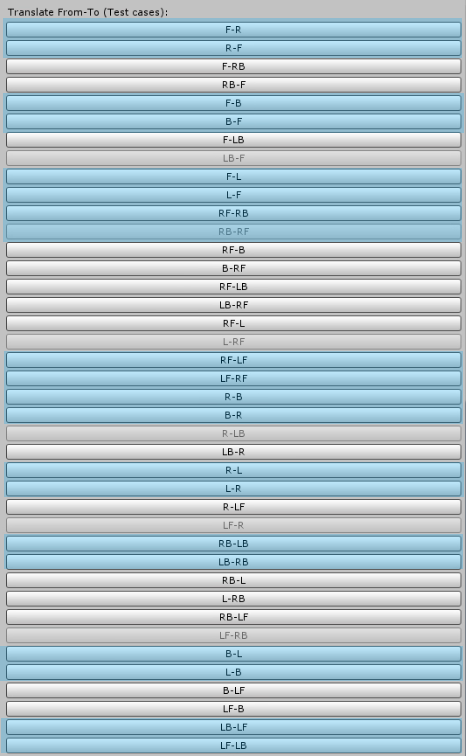
\includegraphics[width=0.7\linewidth]{figures/pilot2_tutorial_control_panel_highlighted}
	\caption{Control panel}
	\label{fig:pilot2tutorialcontrolpanelhighlighted}
\end{figure}

\begin{figure}
	\centering
	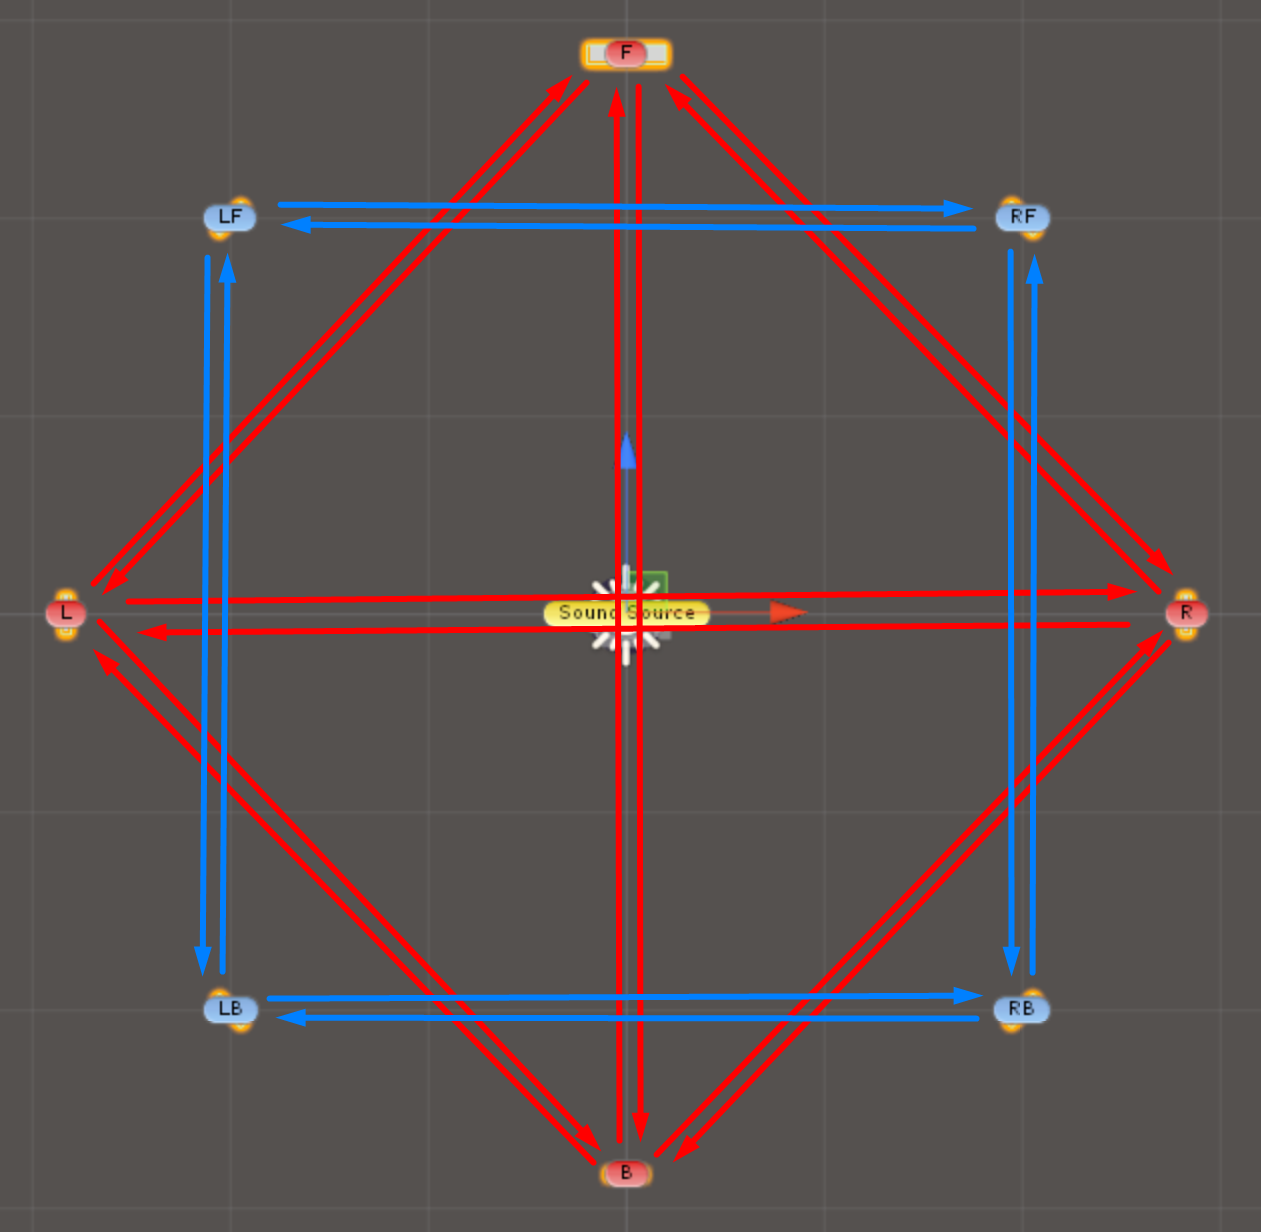
\includegraphics[width=0.7\linewidth]{pilot2_endpoints_tutorial_tranlstaions}
	\caption{Tutorial translations}
	\label{fig:pilot2endpointstutorialtranlstaions}
\end{figure}



After the tutorial translations were demonstrated, participants were asked if they were ready to proceed to the actual experiment. Only one participant asked to repeat some of the translations to gain a better spatial understanding.

In the experiment mode participants were not able to see the building, but would still hear the sounds when it started moving. The wall around the user was visible. The end-points of the translations of the building were always on this wall. Participants were asked to indicate where the building translated from and to with the help of a simulated laser pointer attached to the controller. The details of the controls can be found in Appendix \ref{app:pilot2_controls}.

All 40 translations were initiated in a pseudo-random order for each participant. This order was decided by the experimenter. Each translation could be initiated only once, to make sure no translations were initiated multiple times (after the initiation the button for this translation would be grayed-out and rendered inactive, see Fir. \ref{fig:pilot2tutorialcontrolpanelhighlighted}). The experimenter was responsible for  initiating the translations.
Participants answers were recorded by the system in a CSV file.

When participants went through all the 40 translations, the experiment would end. Experimenter thanked the participants and ask for their feedback concerning the experiment.

\paragraph{Apparatus} The same, as in \ref{study_one} \nameref{study_one}, with addition of 6 \gls{dof} tracked controllers.

\paragraph{Study design}
This study used the repeated measures design with one independent variable - translation paths (40 values).

The building could travel between the total of 8 endpoints. These were moved equidistantly and  placed around the participant (approx. 28.3m away) along the cylinder wall (Fig. \ref{fig:pilot2endpoints}).

\begin{figure}
	\centering
	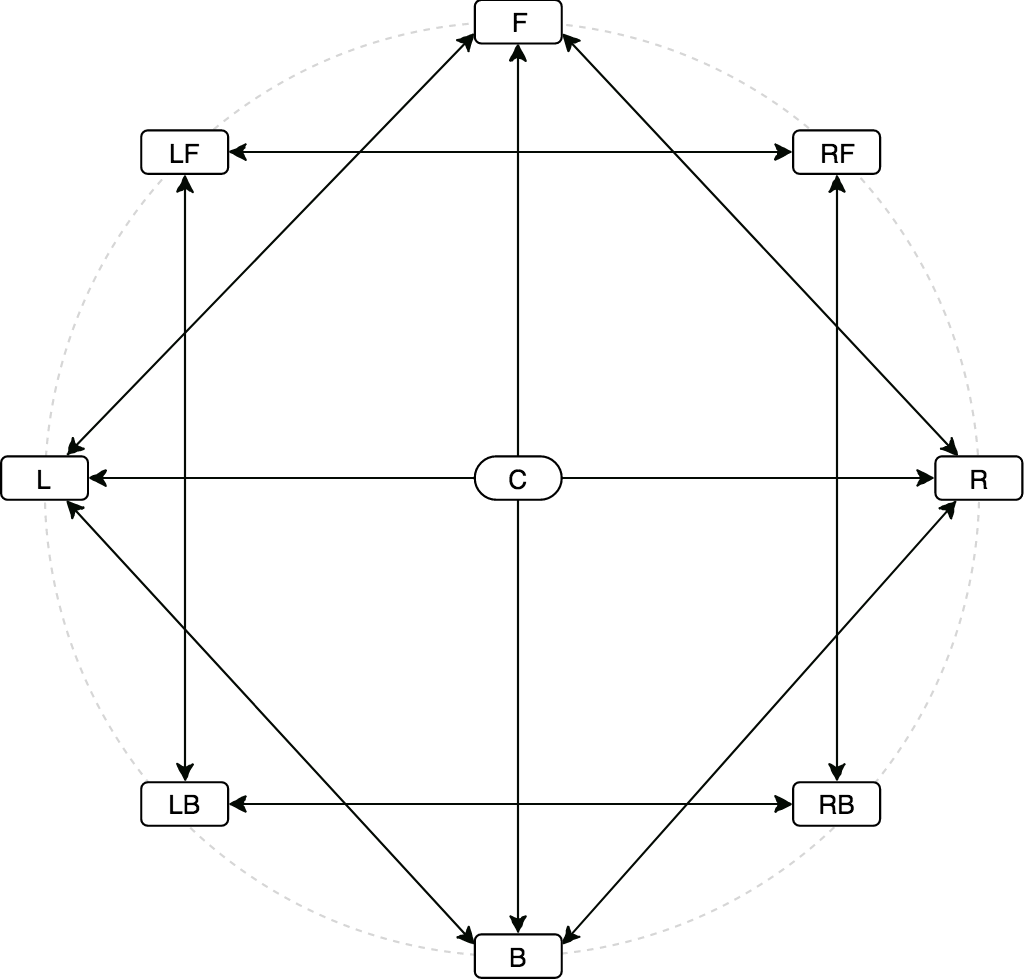
\includegraphics[width=0.7\linewidth]{figures/pilot2_endpoints}
	\caption{Translation endpoints}
	\label{fig:pilot2endpoints}
\end{figure}


The auditory icon of a concrete bock sliding on a concrete surface from the previous experiment was used. 

The translation speed of the building was 30m/s.

\paragraph{Results}

A sample of the collected data can be seen in Fig. \ref{fig:pilot2datasample}. The link to the complete data can be found in Appendix \ref{app:pilot2data_collected}.

The following was collected:
\begin{itemize}
	\item From X, From Y, From Z - start-point of the translation;
	\item To X, To Y, To Z - end-point of the translation;
	\item From Abbreviation, To Abbreviation - name abbreviation of the start- and end-points (i.e. "LB" corresponds to "Left Back");
	\item Translation Start, Translation Finish - time in seconds since the beginning of the game, until the translation started and finished, respectively;
	\item Guess From X, Guess From Y, Guess From Z - participant-perceived start-point of the translation;
	\item Guess To X, Guess To Y, Guess To Z - participant-perceived end-point of the translation;
	\item Guess Start, Guess Finish - time in seconds since the beginning of the game, until the participant indicated the start- and end-points of the translation;
	\item Angle From, Angle To - angle between the C-F (the line between the Center point and the Front point) and C-(From X, 0, From Z), C-(To X, 0, To Z), respectively;
	\item Guess Angle From, Guess Angle To - angle between the C-F and C-(Guess From X, 0, Guess From Z), C-(Guess To X, 0, Guess To Z), respectively;
	\item Divergence Angle From, Divergence Angle To - angular distance between the Angle From and Guess Angle From, Angle To and Guess Angle To, respectively.
\end{itemize}

\begin{figure}
	\centering
	\subfloat{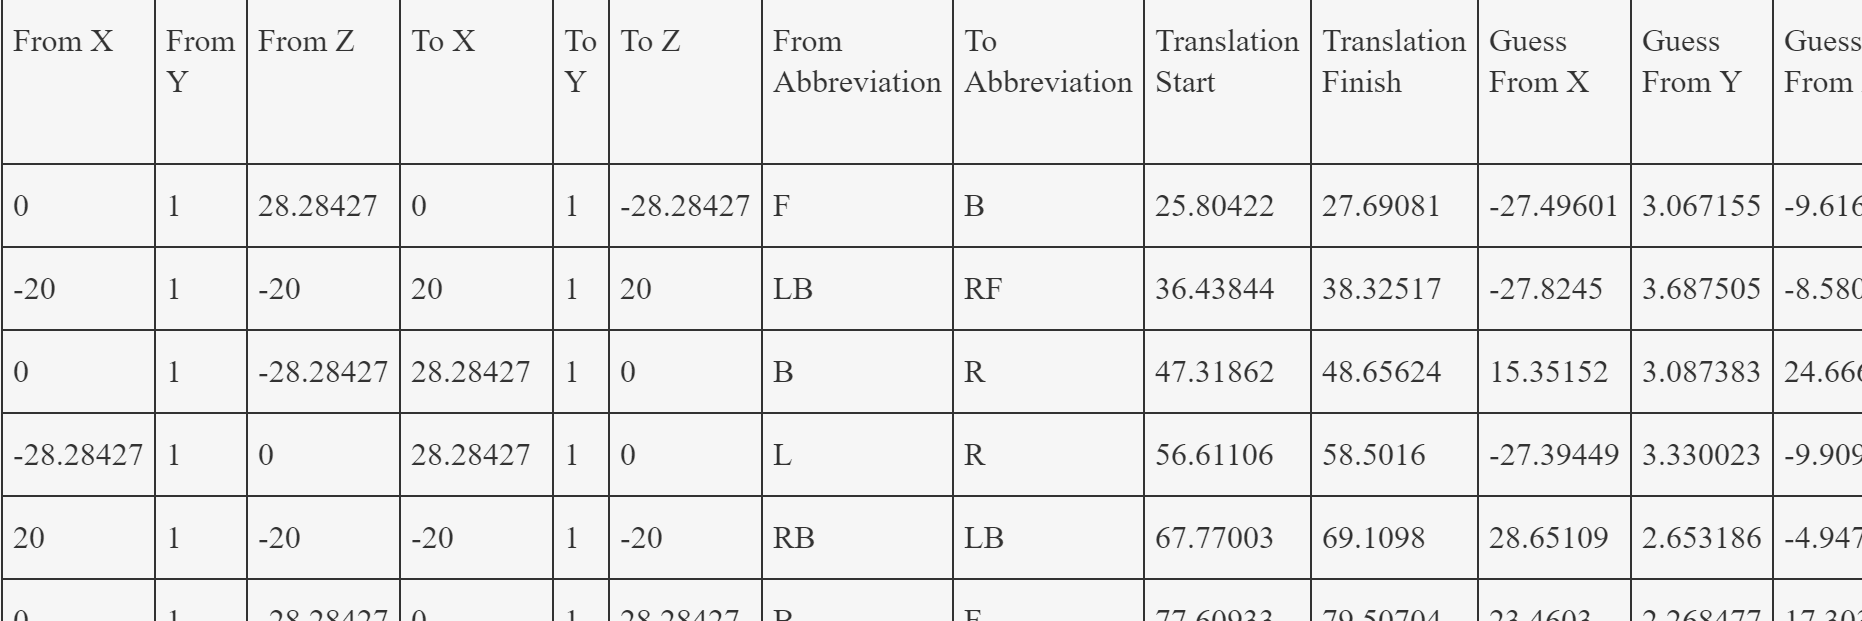
\includegraphics[width=0.7\linewidth]{figures/pilot2_datasample1}}
	\par
	\subfloat{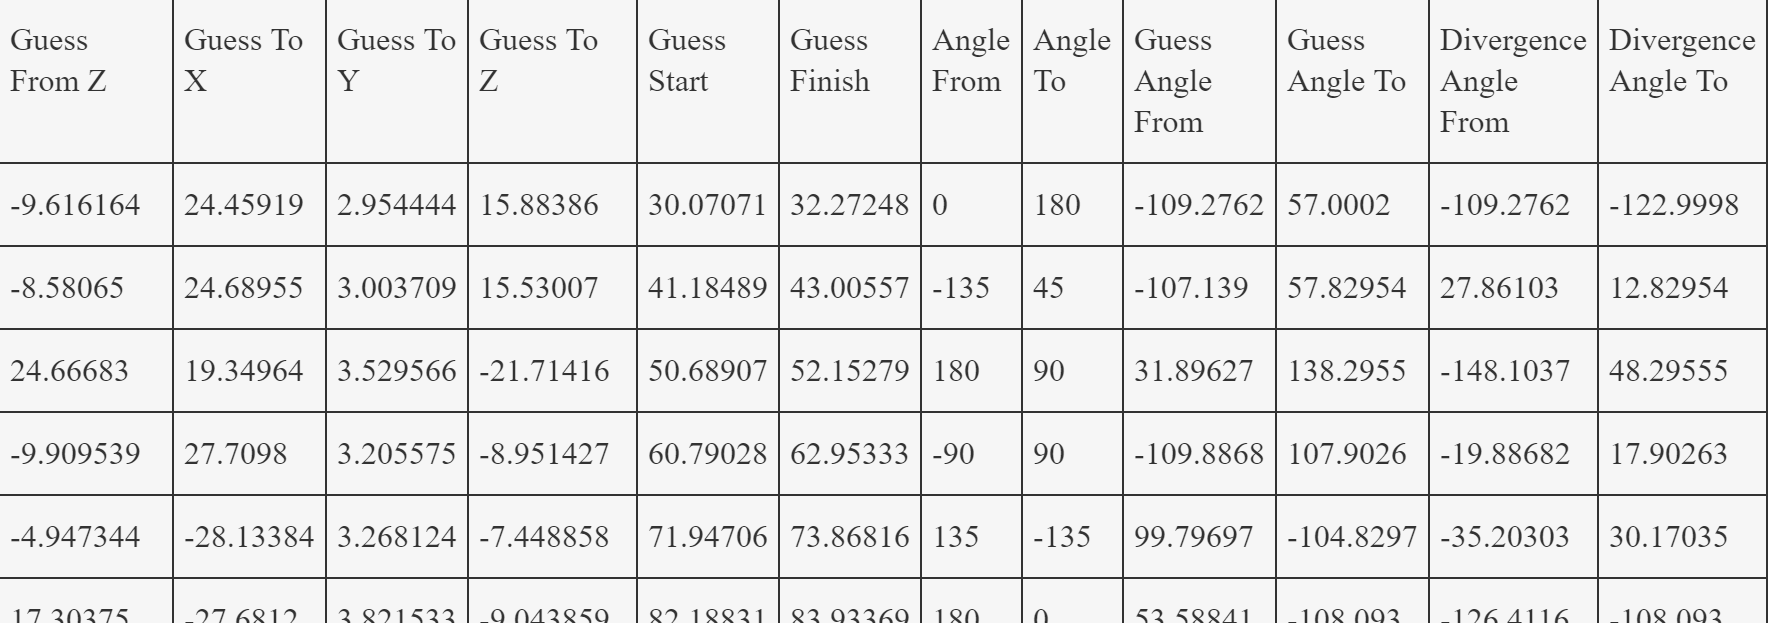
\includegraphics[width=0.7\linewidth]{figures/pilot2_datasample2}}
	\caption{Collected data sample}
	\label{fig:pilot2datasample}
\end{figure}



% Post-questionnaire summary
At least half of the participants reported having trouble to differentiate front and back translations. Some thought the building was always in the back, but decided to give some answers in-front just to balance the results. One participant indicated that everything was "easy and logical" when the building was visible, and unclear when it was not.

\paragraph{Discussion}
% Example visual result w/ explanation
The results of the experiment were represented visually, as seen in the Fig. \ref{fig:b-f}. One visualization was created for each path that the building traveled in the experiment (40 visualizations). These can be found in Appendix \ref{app:pilot2visual_analysis}.

\begin{figure}
	\centering
	\includegraphics[width=0.7\linewidth]{../Studies/SpatialJudgements/Generated/B-F}
	\caption{Example visualization of data for the translation path Back to Front}
	\label{fig:b-f}
\end{figure}

This visualization can be thought of as a top-down projection of the experiment environment.
Individual answers are shown with semi-transparent directional rays of red-blue gradient. The beginning of individual rays is wider and red, the ending - thiner and blue. The transparency value $t$ was approx. equal $7.7$, and was computed as $t = 100 / n_{p}$, where $ n_{p} $ is the number of participants.
The information in the left corner ("PATH") describes the actual translation path: "abbr." - name abbreviation of the path, "act." - actual angles the building traveled from and to. This data is also visualized with the green line, whose end-points are marked with big green circles and "From", and "To" labels.
The information in the right corner ("STATS (deg.)") gives the statistical data for this path in degrees: "mean" - mean values for the "Guess From" and "Guess To" entries, respectively. This information is also visualized with the red line, whose end-points are marked with small red circles and "m.From", and "m.To" (which stand for: "mean From" and "mean To", respectively).
Start- end end-points of translations are marked with their respective name abbreviations and deviation angles from the Front direction.

On this example we see the visualization of the guesses made by participants when the building traveled from Back to Front (B-F). A certain number of participants have guessed correctly, which is indicated by a brighter (or less transparent) overlay of the directional rays. The mean value goes from approx. $152.3\degree$ to approx. $- 30.8\degree$. The error of $\pm 45\degree$ can be considered negligible due to the limitations of the stereo headphones and the absence of the visual cues. At least 5 participants have guessed incorrectly, and at least one thought that the building moved from Front to Back, which is indicated by the red ray ending starting at the F point and going straight down.


% Interpretation of the results
The mean values for 29 out of 40 translations were close to the actual translation paths, if we assume the result being in the range of the negligible error of $\pm 45\degree$ as close. % Green dot
Among the rest, 6 translations can be considered close, if we eliminate the front-to-back confusion by mirroring either one, or both the start and finish endpoints along the imaginary L-R line.
% Mean deviation for deviation of start and end /points // <- estimate - apparently, not useful for the stats analysis: https://en.wikipedia.org/wiki/Unbiased_estimation_of_standard_deviation

% Conclusion
Regardless, of many erroneous guesses, the analysis shows promise for the given setup, and, considering the previous success of \cite{gutwin_chalk_2011} in representing spatial information with auditory cues through the stereo headphones, as well as the fact that in the final study participants will have visual cues to aid them in finding the sound source, and the fact that they won't be forced to always face the same direction, this approach deserves a further analysis.

%\subparagraph{Limitations}

% Number of participants














\section{Workspace Awareness in Immersive Virtual Reality}
\label{final_study}
% Goal of the study
The goal of this study was to analyze \gls{wa} that participants have of others present in the same immersive \gls{vr} environment. Participants were presented with a primary and secondary tasks. Primary task was tracing 3D models with a 3D brush, and secondary task was a \gls{wa} task - reporting changes to the environment.
%\paragraph{Methods}
The evaluated aspects of \gls{wa} were participants’ reaction speed when provided with different types of awareness presentation (audio and/or visual cues about the environment).

\paragraph{Participants}
12 participants (8 men and 4 women) were recruited among friends, employees from the chair, and students from the \gls{tum}; ages ranged from 22 to 32 (mean 25.2, std. 2.5). Only one participant reported having "partially" good hearing, others reported good hearing. 3 people reported to be familiar with \gls{vr} technology, among them, one person reported being a proficient gamer and one - having partaken in driving simulator studies. Participants were a mix of gamers, non-gamers, and casual gamers. Participants were also equally distributed among people who had experience with \gls{vr}, those who had some experience, and those who had no prior experience. Two reported being online gamers, and another two - occasional online gamers. Only one person had prior experience with architecture, and had worked in the field. One participant tried 3D drawing in the system before, but otherwise none had seen the system before, or took part in the previous studies.

\paragraph{Procedure}
Participants were given a written and verbal introduction to the experiment,
and were asked to sign the consent form for using their data.
Next, they were placed in the immersive \gls{vr} environment, which implemented 2 modes: tutorial and experiment (Fig \ref{fig:finalstudy_immersive_vr_environment}). In the tutorial mode, only one building (the clock tower) and the test tracing shape would be visible.
Participants learned how to use the 3D voxel brush for tracing the shapes (Fig. \ref{fig:finalstudyvoxeldrawing}), the laser pointer to indicate they noticed changes to the environment, and the minimap to locate the moving buildings. Following that, the auditory cues were introduced, and the differences between the tutorial and the actual experiment part were explained. Participants went through a small scenario, resembling the experiment, where they were asked to trace a pillar, and in the meanwhile try to catch the moving building a couple of times. They were also asked to keep track of how the building sounds and where it is visually.

\begin{figure}
	\centering
	
	\subfloat[Tutorial environment, the clock tower]{\includegraphics[scale=.29]{D://Documents/studies/ss18/Thesis/tum-thesis-latex/figures/finalstudy_environment_tutorial}}
	\par
	\subfloat[Experiemnt environment, the clock tower]{\includegraphics[scale=.29]{D://Documents/studies/ss18/Thesis/tum-thesis-latex/figures/finalstudy_environment2}}
	\par
	\subfloat[Experiemnt environment, the tracing shape]{\includegraphics[scale=.29]{D://Documents/studies/ss18/Thesis/tum-thesis-latex/figures/finalstudy_environment}}
	
	\caption{Virtual environment}
	\label{fig:finalstudy_immersive_vr_environment}
\end{figure}

\begin{figure}
	\centering

	\subfloat[Tracing shape]{\includegraphics[width=0.7\linewidth]{figures/finalstudy_voxeldrawing1}}
	\par
	\subfloat[Partially traced shape]{\includegraphics[width=0.7\linewidth]{figures/finalstudy_voxeldrawing2}}
	\par
	\subfloat[Tracing shape and voxel drawing side-by-side]{\includegraphics[width=0.7\linewidth]{figures/finalstudy_voxeldrawing3}}

	\caption{Voxel drawing}
	\label{fig:finalstudyvoxeldrawing}
\end{figure}


During the actual experiment, each participant was tested in each of the 3 test groups: \textit{Minimap and Sound}, \textit{Sound Only}, and \textit{Minimap Only}. Participants were instructed to keep focus on their main task and treat the experiment not as a test of their abilities to notice all the moving buildings, but rather as a test to check how good the system was in informing them of these changes. 
When participants were done with a shape, they would voice this to the experimenter, and he would save the current voxel drawing, and switch the tracing shape to the next one.
At the end of the experiment, participants were asked to fill in a self-report questionnaire.
Participants did not rest between the different conditions. 
After the end of the experiment, participants were asked to fill out a questionnaire (Appendix \ref{app:final_study_questionnaire}).

\paragraph{Task}
Participants were asked to follow a scenario, in which there were 2 architects (A1 and A2), who performed their separate tasks in the same urban district (\ref{fig:urbandistrict}) in \gls{vr}. A1 (participant) had 2 tasks, primary and secondary. The primary task was to trace given 3D shapes with a 3D voxel brush, which was implemented for one of the tracked 6-\gls{dof} controllers (see Fig. ). Meanwhile, A2 (simulated invisible agent) could translate any building in the district to any other part of the district at any time. The secondary (workspace awareness) task of A1 was to keep track of changes to the environment and point them out with a virtual laser pointer (another tracked 6-\gls{dof} controller). The details of controls can be found in Appendix \ref{app:finalstudy_controls}

\begin{figure}
	\centering
	\includegraphics[width=0.7\linewidth]{figures/urban_district}
	\caption{Simulated urban district for the \gls{wa} study}
	\label{fig:urbandistrict}
\end{figure}


\paragraph{Apparatus} The same, as in \ref{study_two} \nameref{study_two}.

% Study Factors and Conditions: what my factors are, conditions == independent variables' values
% + Repeated-measures design?
\paragraph{Study design}
%\textit{Experimental Design} 
This study followed the repeated measures design with one independent variable - the type of awareness presentation. 3 controlled awareness presentations were used
\begin{itemize}
	\item minimap of the district (\ref{fig:minimap_controller});
	\item auditory cues emitted by translating buildings in the scene (sound of a concrete block sliding on a concrete surface);
	\item combination of the minimap and auditory cues.
\end{itemize}

Awareness presentations were rotated for each participant, so that each presentation was seen in the same position equal number of times. 
Each awareness presentation was tested for 10 minutes, during which exactly 8 buildings were randomly chosen and translated. In total, 24 data points were measured per participant in each session. Data collected were the reaction speed in determining the position of a moving building (catching it), along with 3D drawings created by participants. If the participant failed to catch the building, the reaction time was recorded as 0.

% TODO: separate screenshot of the minimap controller
\begin{figure}[h]
	\centering
	\includegraphics[width=0.7\linewidth]{figures/placeholders/minimap_controller}
	\caption{Controller with the minimap}
	\label{fig:minimap_controller}
\end{figure}

The total of 13 tracing shapes were prepared for the participants: 1 tutorial shape and 12 experiment shapes (Appendix \ref{app:finalstudy_tracingshapes}).
Participants went through them in the same order at a pace that felt comfortable to them.

\paragraph{Gutwin vs our study}
Since, this study extends upon \cite{gutwin_chalk_2011}, this paragraph provides the comparison of the two.
The main difference between - workspace is no longer a 2D plane, but an immersive 3D \gls{vr} environment. An important change here was the fact that participants were able to look around at the workspace, and notice some changes to the environment, even without the help of the minimap or auditory cues. 
% TODO: also, the fact that the head was tracked and this influenced the sound behaviour

Second distinction was in the primary task of the participant and the simulated agent. In \cite{gutwin_chalk_2011} the participant performed the same task, as an agent: drawing with chalk. Additionally, the participant's actions emit the same sound at a lower volume as the agent's actions. In this study, the primary task of the participant is - 3D drawing with voxels. This activity doesn't emit any sound. It is also different from the agent's task - translation of buildings in the urban district. Nevertheless, the tasks are still contextually related with regards to the architectural activity in urban environment.

In terms of the \gls{wa} framework, \cite{gutwin_chalk_2011} aim to answer the \textit{What?} and \textit{Where?} questions about the workspace: what is being done, and where is it being done. This study follows the same idea. In terms of levels of \gls{sa}, this study touches on all 3 levels: 
\begin{enumerate}
	\item Perception: participant realizes that something is happening in the environment;
	\item Cognition: they understand that it is a building moving, and can locate;
	\item Projection: participant sees or hears the way that building is moving, and based on this, tries to catch it at its next position.
\end{enumerate}

\cite{gutwin_chalk_2011} do not specify the details of their spatial sound, however, since it was a 2D study, it is plausible that all sounds originate in the same plane, we will call it sound plane. In case of \cite{gutwin_chalk_2011} this plane can be positioned in 3 different ways: vertically, horizontally, or somewhere in-between (Fig. \ref{fig:gutwinvsmystudysoundplane}a). In all cases, where the plane is positioned in an orientation that is different from the orientation of the screen, participants would have to build a mapping between for the interface. In this study, sounds are also emitted from the same plane, which is positioned horizontally (Fig. \ref{fig:gutwinvsmystudysoundplane}b).

Other similarities between the two studies include: the study design, the object of analysis (\gls{wa}), and the use of auditory icons as auditory cues.

% TODO: re-draw
\begin{figure}[h]
	\centering
	\includegraphics[width=0.7\linewidth]{figures/gutwin_vs_my_study_sound_plane}
	\caption{\cite{gutwin_chalk_2011} sound plane vs this study}
	\label{fig:gutwinvsmystudysoundplane}
\end{figure}

% TODO: linebreak
\begin{table}[h]
  \caption{Study comparison}
  \label{table:study_comp}
  \begin{tabular}{|l|l|l|}
  \hline
                             & \textbf{Shared chalkboard application}                & \textbf{\gls{wa} in \gls{vr}}           \\ \hline
  \textbf{Workspace dimensions}				 & 2D									   & 3D \\ \hline
  \textbf{Participant's primary (distraction) task} & The same as the primary for the simulated agent & Contextually related \\ \hline
  \textbf{Sound plane}      & Not specified             & Horizonatal          \\ \hline
  \textbf{Type of auditory cues}                 & Auditory icons        & Auditory icons       \\ \hline
  \textbf{Object of analysis}         & Workspace awareness   & Workspace Awareness  \\ \hline
	\textbf{Attentional demand}         & Variable difficulty of the tracing activity   & Variable difficulty of the tracing activity; shift of focus from the participant's personal evaluation to the system evaluation; personal motivation to see their 3D drawings \\ \hline
	  \textbf{Radar size}         & Variable (small, medium, large)   & Constant (medium)  \\ \hline
	    \textbf{Workspace clutter}         & Variable (none, sparse, dense)   & Constant (dense)  \\ \hline
	    \textbf{Measurements collected}         & Accuracy in determining when, where, and what type of action occurred   & Accuracy in determining where the action occurred  \\ \hline
  \end{tabular}
\end{table}

\paragraph{Results}
A sample of the collected data can be seen in Fig. \ref{fig:finalstudydataexample}. The link to the complete data can be found in Appendix \ref{app:final_study_data_collected}.

The following was collected:
\begin{itemize}
	\item Translation id - unique ID number for the translation, which was constructed in the following way: yyyyMMddHHmmssffff (where "yyyy" is the year, "MM" is the month, and so on);
	\item Reaction time - time in seconds between the start of a random translation, until it was caught. If the translation was not noticed by the a participant, or they were not able to catch it, the assigned value is 0;
	\item Group - number code for different experiment groups: 1 - \textit{Minimap and Sound}, 2 - \textit{Sound Only}, 3 - \textit{Minimap Only}.
\end{itemize}

\begin{figure}
	\centering
	\includegraphics[width=0.7\linewidth]{figures/final_study_data_example}
	\caption{Data collected for a participant}
	\label{fig:finalstudydataexample}
\end{figure}

When asked to rate different awareness presentations with an integer score from the most (1) to the least (3) useful, participants gave the feedback, shown in Fig. \ref{fig:finalstudyawarenesspresentationuserpreference}. It was allowed to give the same rating to different presentations (i.e. some participants ranked \textit{Minimap and Sound} and \textit{Sound Only} presentations with the score - 1).

\begin{figure}
	\centering
	\includegraphics[width=0.7\linewidth]{figures/final_study_awareness_presentation_user_preference}
	\caption{}
	\label{fig:finalstudyawarenesspresentationuserpreference}
\end{figure}

Most participants managed to trace the first 3-4 shapes, only one was able to finish 6.

\paragraph{Discussion}
Due to a bug in the implementation, sound wouldn't play sometimes for the first translation in the \textit{Sound Only}, \textit{Minimap and Sound}, or both groups. The entries where the sound did not play were removed from the dataset prior to its analysis. Additionally, to make group observations comparable, in every group, where the sound did play on the first translation, or, like in case with the \textit{Minimap Only} group, the sound was never supposed to play, the last data entry for the group was removed. This way, experiment went from 8 observations per group for each participant to 7.

The visual analysis shows that around $1/4$th of all the translations were not caught: 11 from Group 1, 19 from Group 2, and 26 from Group 3 (Fig. \ref{fig:histograms_combined}, \ref{fig:distributions_freqReaction0}).

Side-by-side distributions clearly indicate that Groups 1 and 2 took less time for participants to catch them (see the violin diagram in Fig \ref{fig:distributions_violin}). Generally, the distribution of the first two groups suggests their relative similarity. The fact that the \textit{Sound Only} group has the smallest reaction times could possibly be an error and the result of a building simply being in the participant's sight. The elongated top-handle of the distribution for the \textit{Sound Only} group could indicate that it was harder to catch the building after noticing it for the first time, which also correlates with the observations of the users during the experiment.

In general, it was observed that it was mostly due to the building or the minimap being in the participants' sight that they were able to spot the moving building in the \textit{Minimap Only} group. By contrast, in case of the groups that relied on the auditory cues, participants were always informed of translations happening, even if they had difficulties exactly locating it (i.e. in the \textit{Sound Only} group).

% TODO: about how the performance should also be judged by how focused the participants were on their main task 
% + figures of some of the voxel drawings (side-by-sides of the same shape to prove the point).

The results of the analysis and participant-feedback suggest that the additional auditory cues help users to improve their awareness of the workspace. The best best awareness presentation was the \textit{Minimap and Sound} group, followed by \textit{Sound Only} and \textit{Minimap Only}.

Statistical summary for each group can be found in Table \ref{tab:final_study_stats}.

\begin{figure}
	\centering
	
	\subfloat[Combined histogram]{\label{fig:histograms_combined}\includegraphics[scale=.15]{D:/Documents/studies/ss18/Thesis/Studies/WorkspaceAwareness/RplotHistogram.png}}
	
	\begin{comment}
		\subfloat[Group 1]{\label{fig:distributions_g1}\includegraphics[scale=.15]{D:/Documents/studies/ss18/Thesis/Studies/WorkspaceAwareness/RplotHistogramGroup1.png}}
	
		\par \smallskip
		\subfloat[Group 2]{\label{fig:histograms_g2}\includegraphics[scale=.15]{D:/Documents/studies/ss18/Thesis/Studies/WorkspaceAwareness/RplotHistogramGroup2.png}}
		\subfloat[Group 3]{\label{fig:histograms_g3}\includegraphics[scale=.15]{D:/Documents/studies/ss18/Thesis/Studies/WorkspaceAwareness/RplotHistorgramGroup3.png}}
	\end{comment}
	
	\subfloat[Uncaught buildings]{\label{fig:distributions_freqReaction0}\includegraphics[scale=.15]{D:/Documents/studies/ss18/Thesis/Studies/WorkspaceAwareness/RplotFreqColorReaction0.png}}
	
	\par \smallskip
	\subfloat[Side-by-side comparison of reaction time, excluding uncaught buildings]{\label{fig:distributions_violin}\includegraphics[scale=.15]{D:/Documents/studies/ss18/Thesis/Studies/WorkspaceAwareness/RplotViolinNon0.png}}
	
	\caption{Data distributions}
	\label{fig:histograms}
\end{figure}
	
\begin{comment}
	\begin{figure}
	\centering
	
	\subfloat[Side-by-side comparison of reaction time]{\label{fig:distributions_violin}\includegraphics[scale=.15]{D:/Documents/studies/ss18/Thesis/Studies/WorkspaceAwareness/RplotViolinNon0.png}}
	\subfloat[Uncaught buildings]{\label{fig:distributions_freqReaction0}\includegraphics[scale=.15]{D:/Documents/studies/ss18/Thesis/Studies/WorkspaceAwareness/RplotFreqColorReaction0.png}}
	
	\label{fig:distributions}
	\caption{Other data distributions}
\end{figure}
\end{comment}

\begin{table}[h]
	\label{tab:final_study_stats}
	\caption{Statistical summary}
	
	\begin{tabular}{|l|l|l|l|}
		\hline
		& \textbf{Group 1: Minimap and Sound} & \textbf{Group 2: Sound Only} & \textbf{Group 3: Minimap Only} \\ \hline
		\textbf{Mean (sec.)}  & 4.662725                            & 4.700911                     & 6.61726                        \\ \hline
		\textbf{St. dev. (sec.)}  & 2.266442                            & 2.483499                     & 2.73528                        \\ \hline
		\textbf{Range (sec.)} & {[}1.865601, 11.195500{]}           & {[}1.567505, 13.192500{]}    & {[}1.890381, 14.635010{]}      \\ \hline
		\textbf{Num. caught}  & 73                                  & 65                           & 58                             \\ \hline
	\end{tabular}
\end{table}
% !TeX root = ../main.tex
% Add the above to each chapter to make compiling the PDF easier in some editors.

\chapter{Conclusion}

% ...

% Future work, etc.
\subparagraph[Future work]{}
% the fact that we only sample the level 1 SA/WA (we won't be going into sampling direction of translation guesses from the participants)
% could also try to describe it according to WA framework
% frame drop
\textit{Frame rate} The implementation of the voxel drawing system was not aimed at maximizing performance, as the result the frame rate dropped to around 70 FPS, when completing some of the shapes (i.e. the Low Poly Trees). One participants indicated that they felt a little bit dizzy due to this problem at one point.

\textit{Minimap} Some users indicated that the minimap implementation was not the most convenient, especially in the \textit{Minimap Only}, where to monitor the map they had to take their attention of the main task. While this will most likely be the case in any implementation, a possible solution would be to see the effects of having the minimap attached to the users head in a non-obstructive way.

% TODO: Support the Gutwin findings; his participants also found both awareness displays to be the most useful setup; Also, address this in abstract, too.
% TODO: add more chapters here

\appendix{}

\microtypesetup{protrusion=false}
\listoffigures{}
\listoftables{}
\microtypesetup{protrusion=true}
\printbibliography
\printglossary[type=\acronymtype,title=Abbreviations]

\begin{appendices}
	
\chapter{Questionnaire Data for Pilot 2: Spatial Judgment}
\label{app:pilot2questionnaire_data}

% \newline and \linebreak didn't work for the line break inside a cell

\begin{table}[]
	\begin{tabular}{|l|l|l|l|l|l|}
		\hline
		\textbf{Participant \#} & \textbf{Gender} & \textbf{Age} & \textbf{Agree/Disagree: I have a good amount of experience in VR} & \textbf{A/D: I have good hearing} & \textbf{A/D: I am a regular online gamer} \\ \hline
		1                       & Male            & 23           & Strongly Agree                                                    & Agree                             & Agree                                     \\ \hline
		2                       & Male            & 29           & Strongly Agree                                                    & Strongly Agree                    & Neutral                                   \\ \hline
		3                       & Male            & 29           & Disagree                                                          & Strongly Agree                    & Strongly Disagree                         \\ \hline
		4                       & Male            & 30           & Strongly Agree                                                    & Disagree                          & Agree                                     \\ \hline
		5                       & Male            & 22           & Strongly Agree                                                    & Neutral                           & Disagree                                  \\ \hline
		6                       & Male            & 22           & Strongly Agree                                                    & Agree                             & Agree                                     \\ \hline
		7                       & Male            & 21           & Strongly Agree                                                    & Strongly Agree                    & Disagree                                  \\ \hline
		8                       & Female          & 20           & Agree                                                             & Neutral                           & Disagree                                  \\ \hline
		9                       & Female          & 24           & Strongly Agree                                                    & Agree                             & Agree                                     \\ \hline
		10                      & Female          & 32           & Disagree                                                          & Agree                             & Disagree                                  \\ \hline
		11                      & Female          & 50           & Agree                                                             & Disagree                          & Strongly Disagree                         \\ \hline
		12                      & Male            & 54           & Disagree                                                          & Neutral                           & Agree                                     \\ \hline
		13                      & Male            & 27           & Strongly Agree                                                    & Strongly Agree                    & Strongly Agree                            \\ \hline
	\end{tabular}
\end{table}	

\chapter{Visual Analysis for Pilot 2: Spatial Judgment}
\label{app:pilot2visual_analysis}

\begin{figure}
	%\centering
	
	\subfloat[B-F]{\includegraphics[scale=0.075]{D:/Documents/Projects/Unity/Sound-Study/Generated/B-F.png}}\hfill
	\subfloat[B-L]{\includegraphics[scale=0.075]{D:/Documents/Projects/Unity/Sound-Study/Generated/B-L.png}}
	\par\smallskip
	\subfloat[B-LF]{\includegraphics[scale=0.075]{D:/Documents/Projects/Unity/Sound-Study/Generated/B-LF.png}}\hfill
	\subfloat[B-R]{\includegraphics[scale=0.075]{D:/Documents/Projects/Unity/Sound-Study/Generated/B-R.png}}
	\par\smallskip
	\subfloat[B-RF]{\includegraphics[scale=0.075]{D:/Documents/Projects/Unity/Sound-Study/Generated/B-RF.png}}\hfill
	\subfloat[F-B]{\includegraphics[scale=0.075]{D:/Documents/Projects/Unity/Sound-Study/Generated/F-B.png}}
\end{figure}
\begin{figure}	
	%	\centering
	
	\subfloat[F-L]{\includegraphics[scale=0.075]{D:/Documents/Projects/Unity/Sound-Study/Generated/F-L.png}}\hfill
	\subfloat[F-R]{\includegraphics[scale=0.075]{D:/Documents/Projects/Unity/Sound-Study/Generated/F-R.png}}
	\par\smallskip
	\subfloat[L-B]{\includegraphics[scale=0.075]{D:/Documents/Projects/Unity/Sound-Study/Generated/L-B.png}}\hfill
	\subfloat[F-LB]{\includegraphics[scale=0.075]{D:/Documents/Projects/Unity/Sound-Study/Generated/F-LB.png}}
	\par\smallskip
	\subfloat[F-RB]{\includegraphics[scale=0.075]{D:/Documents/Projects/Unity/Sound-Study/Generated/F-RB.png}}\hfill
	\subfloat[L-F]{\includegraphics[scale=0.075]{D:/Documents/Projects/Unity/Sound-Study/Generated/L-F.png}}
\end{figure}
\begin{figure}
	%	\centering
	
	\subfloat[L-R]{\includegraphics[scale=0.075]{D:/Documents/Projects/Unity/Sound-Study/Generated/L-R.png}}\hfill
	\subfloat[L-RB]{\includegraphics[scale=0.075]{D:/Documents/Projects/Unity/Sound-Study/Generated/L-RB.png}}
	\par\smallskip
	\subfloat[L-RF]{\includegraphics[scale=0.075]{D:/Documents/Projects/Unity/Sound-Study/Generated/L-RF.png}}\hfill
	\subfloat[LB-F]{\includegraphics[scale=0.075]{D:/Documents/Projects/Unity/Sound-Study/Generated/LB-F.png}}
	\par\smallskip
	\subfloat[LB-LF]{\includegraphics[scale=0.075]{D:/Documents/Projects/Unity/Sound-Study/Generated/LB-LF.png}}\hfill
	\subfloat[LB-R]{\includegraphics[scale=0.075]{D:/Documents/Projects/Unity/Sound-Study/Generated/LB-R.png}}
\end{figure}
\begin{figure}
	%	\centering
	
	\subfloat[LB-RB]{\includegraphics[scale=0.075]{D:/Documents/Projects/Unity/Sound-Study/Generated/LB-RB.png}}\hfill
	\subfloat[LB-RF]{\includegraphics[scale=0.075]{D:/Documents/Projects/Unity/Sound-Study/Generated/LB-RF.png}}
	\par\smallskip
	\subfloat[LF-LB]{\includegraphics[scale=0.075]{D:/Documents/Projects/Unity/Sound-Study/Generated/LF-LB.png}}\hfill
	\subfloat[LF-B]{\includegraphics[scale=0.075]{D:/Documents/Projects/Unity/Sound-Study/Generated/LF-B.png}}
	\par\smallskip
	\subfloat[LF-R]{\includegraphics[scale=0.075]{D:/Documents/Projects/Unity/Sound-Study/Generated/LF-R.png}}\hfill
	\subfloat[LF-RB]{\includegraphics[scale=0.075]{D:/Documents/Projects/Unity/Sound-Study/Generated/LF-RB.png}}
\end{figure}
\begin{figure}
	%	\centering
	
	\subfloat[LF-RF]{\includegraphics[scale=0.075]{D:/Documents/Projects/Unity/Sound-Study/Generated/LF-RF.png}}\hfill
	\subfloat[R-F]{\includegraphics[scale=0.075]{D:/Documents/Projects/Unity/Sound-Study/Generated/R-F.png}}
	\par\smallskip
	\subfloat[R-B]{\includegraphics[scale=0.075]{D:/Documents/Projects/Unity/Sound-Study/Generated/R-B.png}}\hfill
	\subfloat[R-L]{\includegraphics[scale=0.075]{D:/Documents/Projects/Unity/Sound-Study/Generated/R-L.png}}
	\par\smallskip
	\subfloat[R-LB]{\includegraphics[scale=0.075]{D:/Documents/Projects/Unity/Sound-Study/Generated/R-LB.png}}\hfill
	\subfloat[R-LF]{\includegraphics[scale=0.075]{D:/Documents/Projects/Unity/Sound-Study/Generated/R-LF.png}}
\end{figure}
\begin{figure}
	\centering
	
	\subfloat[RB-F]{\includegraphics[scale=0.075]{D:/Documents/Projects/Unity/Sound-Study/Generated/RB-F.png}}\hfill
	\subfloat[RB-L]{\includegraphics[scale=0.075]{D:/Documents/Projects/Unity/Sound-Study/Generated/RB-L.png}}
	\par\smallskip
	\subfloat[RB-LB]{\includegraphics[scale=0.075]{D:/Documents/Projects/Unity/Sound-Study/Generated/RB-LB.png}}\hfill
	\subfloat[RB-LF]{\includegraphics[scale=0.075]{D:/Documents/Projects/Unity/Sound-Study/Generated/RB-LF.png}}
	\par\smallskip
	\subfloat[RF-B]{\includegraphics[scale=0.075]{D:/Documents/Projects/Unity/Sound-Study/Generated/RF-B.png}}\hfill
	\subfloat[RB-RF]{\includegraphics[scale=0.075]{D:/Documents/Projects/Unity/Sound-Study/Generated/RB-RF.png}}
\end{figure}
\begin{figure}
	\centering
	
	\subfloat[RF-L]{\includegraphics[scale=0.075]{D:/Documents/Projects/Unity/Sound-Study/Generated/RF-L.png}}\hfill
	\subfloat[RF-LB]{\includegraphics[scale=0.075]{D:/Documents/Projects/Unity/Sound-Study/Generated/RF-LB.png}}
	\par\smallskip
	\subfloat[RF-RB]{\includegraphics[scale=0.075]{D:/Documents/Projects/Unity/Sound-Study/Generated/RF-RB.png}}\hfill
	\subfloat[RF-LF]{\includegraphics[scale=0.075]{D:/Documents/Projects/Unity/Sound-Study/Generated/RF-LF.png}}
	%	\caption{Visual analysis of the results, pilot 2, pt.2}
	%	\label{fig:pilot2resltsanalysispt2}
\end{figure}



\end{appendices}

\end{document}
